\documentclass[11pt]{article}

% The four macros of the header standard; tools/zenodo/publish_revision.py patches them when it reserves the DOI.
\newcommand{\doctype}{Preprint}
\newcommand{\docversion}{v1.00.000}
\newcommand{\docdate}{8 November 2026}
\newcommand{\versiondoi}{10.5281/zenodo.24053160}
\newcommand{\conceptdoi}{10.5281/zenodo.24053159}
\newcommand{\docidentity}{CAOS\_Contraste, the validation of the risk models of a bank}

% The packages and conventions every Contraste manuscript shares (CAOS_MANAGE conventions/manuscript-content-bar.md
% section 2). A document sets its class, the four header macros and \docidentity, then % The packages and conventions every Contraste manuscript shares (CAOS_MANAGE conventions/manuscript-content-bar.md
% section 2). A document sets its class, the four header macros and \docidentity, then % The packages and conventions every Contraste manuscript shares (CAOS_MANAGE conventions/manuscript-content-bar.md
% section 2). A document sets its class, the four header macros and \docidentity, then \input{../_shared/preamble}.
\usepackage[T1]{fontenc}
\usepackage[utf8]{inputenc}
\usepackage{lmodern}
\usepackage{microtype}
\usepackage[a4paper,margin=2.5cm]{geometry}
\usepackage{amsmath,amssymb,amsthm,mathtools,bm}
\usepackage{graphicx}
\usepackage{booktabs,longtable,tabularx,array,multirow}
\usepackage{siunitx}
\usepackage{algorithm}
\usepackage{algpseudocode}
\usepackage{caption,subcaption}
\usepackage{xcolor}
\usepackage[numbers,sort&compress]{natbib}
\usepackage[hidelinks]{hyperref}
\usepackage{cleveref}
\usepackage{orcidlink}

\sisetup{group-separator={,},group-minimum-digits=4,detect-all}
\graphicspath{{figures/}{../figures/}}
\captionsetup{font=small,labelfont=bf}
\setlength{\LTcapwidth}{\textwidth}

% Theorem environments for the Theory sections of the manuscripts.
\newtheorem{proposition}{Proposition}
\newtheorem{lemma}{Lemma}
\newtheorem{corollary}{Corollary}
\theoremstyle{definition}
\newtheorem{definition}{Definition}
\newtheorem{assumption}{Assumption}
\theoremstyle{remark}
\newtheorem{remark}{Remark}

% Notation shared by the documents (each defines it again in its notation table).
\newcommand{\E}{\mathbb{E}}
\newcommand{\Prob}{\mathbb{P}}
\newcommand{\Var}{\operatorname{Var}}
\newcommand{\Cov}{\operatorname{Cov}}
\newcommand{\VaR}{\operatorname{VaR}}
\newcommand{\ES}{\operatorname{ES}}
\newcommand{\PD}{\mathrm{PD}}
\newcommand{\LGD}{\mathrm{LGD}}
\newcommand{\EAD}{\mathrm{EAD}}
\newcommand{\ECL}{\mathrm{ECL}}
\newcommand{\indic}{\mathbf{1}}
\newcommand{\R}{\mathbb{R}}
\newcommand{\dd}{\,\mathrm{d}}

% The page-1 header block (CAOS_MANAGE conventions/manuscript-header-standard.md). The document defines \doctype,
% \docversion, \docdate, \versiondoi, \conceptdoi and \docidentity before this file; the publishing tool patches the four
% macros of the standard when it reserves the version DOI.
\newcommand{\docrepo}{github.com/fsantibanezleal/CAOS\_Contraste}
\newcommand{\headerblock}{%
\begin{center}
\fbox{\parbox{0.94\textwidth}{\small\raggedright
\textbf{\doctype} \quad$\cdot$\quad \docversion, \docdate \quad$\cdot$\quad Licence CC BY 4.0\\[2pt]
CAOS open-research programme \quad$\cdot$\quad \docidentity\\[2pt]
Version DOI \href{https://doi.org/\versiondoi}{\texttt{\versiondoi}} \quad$\cdot$\quad
concept DOI (always latest) \href{https://doi.org/\conceptdoi}{\texttt{\conceptdoi}}\\[2pt]
Not peer reviewed. Source code, data and computational records: \href{https://\docrepo}{\texttt{\docrepo}}
}}
\end{center}
\vspace{4pt}}
.
\usepackage[T1]{fontenc}
\usepackage[utf8]{inputenc}
\usepackage{lmodern}
\usepackage{microtype}
\usepackage[a4paper,margin=2.5cm]{geometry}
\usepackage{amsmath,amssymb,amsthm,mathtools,bm}
\usepackage{graphicx}
\usepackage{booktabs,longtable,tabularx,array,multirow}
\usepackage{siunitx}
\usepackage{algorithm}
\usepackage{algpseudocode}
\usepackage{caption,subcaption}
\usepackage{xcolor}
\usepackage[numbers,sort&compress]{natbib}
\usepackage[hidelinks]{hyperref}
\usepackage{cleveref}
\usepackage{orcidlink}

\sisetup{group-separator={,},group-minimum-digits=4,detect-all}
\graphicspath{{figures/}{../figures/}}
\captionsetup{font=small,labelfont=bf}
\setlength{\LTcapwidth}{\textwidth}

% Theorem environments for the Theory sections of the manuscripts.
\newtheorem{proposition}{Proposition}
\newtheorem{lemma}{Lemma}
\newtheorem{corollary}{Corollary}
\theoremstyle{definition}
\newtheorem{definition}{Definition}
\newtheorem{assumption}{Assumption}
\theoremstyle{remark}
\newtheorem{remark}{Remark}

% Notation shared by the documents (each defines it again in its notation table).
\newcommand{\E}{\mathbb{E}}
\newcommand{\Prob}{\mathbb{P}}
\newcommand{\Var}{\operatorname{Var}}
\newcommand{\Cov}{\operatorname{Cov}}
\newcommand{\VaR}{\operatorname{VaR}}
\newcommand{\ES}{\operatorname{ES}}
\newcommand{\PD}{\mathrm{PD}}
\newcommand{\LGD}{\mathrm{LGD}}
\newcommand{\EAD}{\mathrm{EAD}}
\newcommand{\ECL}{\mathrm{ECL}}
\newcommand{\indic}{\mathbf{1}}
\newcommand{\R}{\mathbb{R}}
\newcommand{\dd}{\,\mathrm{d}}

% The page-1 header block (CAOS_MANAGE conventions/manuscript-header-standard.md). The document defines \doctype,
% \docversion, \docdate, \versiondoi, \conceptdoi and \docidentity before this file; the publishing tool patches the four
% macros of the standard when it reserves the version DOI.
\newcommand{\docrepo}{github.com/fsantibanezleal/CAOS\_Contraste}
\newcommand{\headerblock}{%
\begin{center}
\fbox{\parbox{0.94\textwidth}{\small\raggedright
\textbf{\doctype} \quad$\cdot$\quad \docversion, \docdate \quad$\cdot$\quad Licence CC BY 4.0\\[2pt]
CAOS open-research programme \quad$\cdot$\quad \docidentity\\[2pt]
Version DOI \href{https://doi.org/\versiondoi}{\texttt{\versiondoi}} \quad$\cdot$\quad
concept DOI (always latest) \href{https://doi.org/\conceptdoi}{\texttt{\conceptdoi}}\\[2pt]
Not peer reviewed. Source code, data and computational records: \href{https://\docrepo}{\texttt{\docrepo}}
}}
\end{center}
\vspace{4pt}}
.
\usepackage[T1]{fontenc}
\usepackage[utf8]{inputenc}
\usepackage{lmodern}
\usepackage{microtype}
\usepackage[a4paper,margin=2.5cm]{geometry}
\usepackage{amsmath,amssymb,amsthm,mathtools,bm}
\usepackage{graphicx}
\usepackage{booktabs,longtable,tabularx,array,multirow}
\usepackage{siunitx}
\usepackage{algorithm}
\usepackage{algpseudocode}
\usepackage{caption,subcaption}
\usepackage{xcolor}
\usepackage[numbers,sort&compress]{natbib}
\usepackage[hidelinks]{hyperref}
\usepackage{cleveref}
\usepackage{orcidlink}

\sisetup{group-separator={,},group-minimum-digits=4,detect-all}
\graphicspath{{figures/}{../figures/}}
\captionsetup{font=small,labelfont=bf}
\setlength{\LTcapwidth}{\textwidth}

% Theorem environments for the Theory sections of the manuscripts.
\newtheorem{proposition}{Proposition}
\newtheorem{lemma}{Lemma}
\newtheorem{corollary}{Corollary}
\theoremstyle{definition}
\newtheorem{definition}{Definition}
\newtheorem{assumption}{Assumption}
\theoremstyle{remark}
\newtheorem{remark}{Remark}

% Notation shared by the documents (each defines it again in its notation table).
\newcommand{\E}{\mathbb{E}}
\newcommand{\Prob}{\mathbb{P}}
\newcommand{\Var}{\operatorname{Var}}
\newcommand{\Cov}{\operatorname{Cov}}
\newcommand{\VaR}{\operatorname{VaR}}
\newcommand{\ES}{\operatorname{ES}}
\newcommand{\PD}{\mathrm{PD}}
\newcommand{\LGD}{\mathrm{LGD}}
\newcommand{\EAD}{\mathrm{EAD}}
\newcommand{\ECL}{\mathrm{ECL}}
\newcommand{\indic}{\mathbf{1}}
\newcommand{\R}{\mathbb{R}}
\newcommand{\dd}{\,\mathrm{d}}

% The page-1 header block (CAOS_MANAGE conventions/manuscript-header-standard.md). The document defines \doctype,
% \docversion, \docdate, \versiondoi, \conceptdoi and \docidentity before this file; the publishing tool patches the four
% macros of the standard when it reserves the version DOI.
\newcommand{\docrepo}{github.com/fsantibanezleal/CAOS\_Contraste}
\newcommand{\headerblock}{%
\begin{center}
\fbox{\parbox{0.94\textwidth}{\small\raggedright
\textbf{\doctype} \quad$\cdot$\quad \docversion, \docdate \quad$\cdot$\quad Licence CC BY 4.0\\[2pt]
CAOS open-research programme \quad$\cdot$\quad \docidentity\\[2pt]
Version DOI \href{https://doi.org/\versiondoi}{\texttt{\versiondoi}} \quad$\cdot$\quad
concept DOI (always latest) \href{https://doi.org/\conceptdoi}{\texttt{\conceptdoi}}\\[2pt]
Not peer reviewed. Source code, data and computational records: \href{https://\docrepo}{\texttt{\docrepo}}
}}
\end{center}
\vspace{4pt}}


% Every number the prose quotes is read from the committed outputs by tables/make_tables.py and typeset with \nv{key}.
% generated by tables/make_tables.py: do not edit
\expandafter\def\csname num@abias.fy.i0.anchored\endcsname{0.2}
\expandafter\def\csname num@abias.fy.i0.band\endcsname{0.2}
\expandafter\def\csname num@abias.fy.i0.followed\endcsname{0.2}
\expandafter\def\csname num@abias.fy.i0.identified\endcsname{2.9}
\expandafter\def\csname num@abias.fy.i0.industry\endcsname{2.9}
\expandafter\def\csname num@abias.fy.i0.unfollowed\endcsname{3.0}
\expandafter\def\csname num@abias.fy.i1.anchored\endcsname{0.0}
\expandafter\def\csname num@abias.fy.i1.band\endcsname{0.0}
\expandafter\def\csname num@abias.fy.i1.followed\endcsname{0.0}
\expandafter\def\csname num@abias.fy.i1.identified\endcsname{0.2}
\expandafter\def\csname num@abias.fy.i1.industry\endcsname{0.2}
\expandafter\def\csname num@abias.fy.i1.unfollowed\endcsname{6.0}
\expandafter\def\csname num@abias.fy.i19.anchored\endcsname{0.1}
\expandafter\def\csname num@abias.fy.i19.band\endcsname{0.1}
\expandafter\def\csname num@abias.fy.i19.followed\endcsname{0.1}
\expandafter\def\csname num@abias.fy.i19.identified\endcsname{40.1}
\expandafter\def\csname num@abias.fy.i19.industry\endcsname{40.1}
\expandafter\def\csname num@abias.fy.i19.unfollowed\endcsname{44.1}
\expandafter\def\csname num@abias.fy.i3.anchored\endcsname{1.1}
\expandafter\def\csname num@abias.fy.i3.band\endcsname{1.1}
\expandafter\def\csname num@abias.fy.i3.followed\endcsname{1.1}
\expandafter\def\csname num@abias.fy.i3.identified\endcsname{5.5}
\expandafter\def\csname num@abias.fy.i3.industry\endcsname{5.5}
\expandafter\def\csname num@abias.fy.i3.unfollowed\endcsname{11.2}
\expandafter\def\csname num@abias.fy.i9.anchored\endcsname{0.1}
\expandafter\def\csname num@abias.fy.i9.band\endcsname{0.1}
\expandafter\def\csname num@abias.fy.i9.followed\endcsname{0.1}
\expandafter\def\csname num@abias.fy.i9.identified\endcsname{20.8}
\expandafter\def\csname num@abias.fy.i9.industry\endcsname{20.8}
\expandafter\def\csname num@abias.fy.i9.unfollowed\endcsname{25.9}
\expandafter\def\csname num@abias.pool.i0.anchored\endcsname{0.1}
\expandafter\def\csname num@abias.pool.i0.band\endcsname{0.1}
\expandafter\def\csname num@abias.pool.i0.followed\endcsname{0.1}
\expandafter\def\csname num@abias.pool.i0.identified\endcsname{2.8}
\expandafter\def\csname num@abias.pool.i0.industry\endcsname{2.8}
\expandafter\def\csname num@abias.pool.i0.unfollowed\endcsname{3.2}
\expandafter\def\csname num@abias.pool.i1.anchored\endcsname{1.7}
\expandafter\def\csname num@abias.pool.i1.band\endcsname{1.7}
\expandafter\def\csname num@abias.pool.i1.followed\endcsname{1.7}
\expandafter\def\csname num@abias.pool.i1.identified\endcsname{2.1}
\expandafter\def\csname num@abias.pool.i1.industry\endcsname{2.1}
\expandafter\def\csname num@abias.pool.i1.unfollowed\endcsname{7.9}
\expandafter\def\csname num@abias.pool.i19.anchored\endcsname{29.1}
\expandafter\def\csname num@abias.pool.i19.band\endcsname{29.1}
\expandafter\def\csname num@abias.pool.i19.followed\endcsname{29.1}
\expandafter\def\csname num@abias.pool.i19.identified\endcsname{60.4}
\expandafter\def\csname num@abias.pool.i19.industry\endcsname{60.4}
\expandafter\def\csname num@abias.pool.i19.unfollowed\endcsname{63.0}
\expandafter\def\csname num@abias.pool.i3.anchored\endcsname{5.9}
\expandafter\def\csname num@abias.pool.i3.band\endcsname{5.9}
\expandafter\def\csname num@abias.pool.i3.followed\endcsname{5.9}
\expandafter\def\csname num@abias.pool.i3.identified\endcsname{12.1}
\expandafter\def\csname num@abias.pool.i3.industry\endcsname{12.1}
\expandafter\def\csname num@abias.pool.i3.unfollowed\endcsname{17.4}
\expandafter\def\csname num@abias.pool.i9.anchored\endcsname{15.9}
\expandafter\def\csname num@abias.pool.i9.band\endcsname{15.9}
\expandafter\def\csname num@abias.pool.i9.followed\endcsname{15.9}
\expandafter\def\csname num@abias.pool.i9.identified\endcsname{35.0}
\expandafter\def\csname num@abias.pool.i9.industry\endcsname{35.0}
\expandafter\def\csname num@abias.pool.i9.unfollowed\endcsname{39.1}
\expandafter\def\csname num@abias.x10.i0.anchored\endcsname{0.2}
\expandafter\def\csname num@abias.x10.i0.band\endcsname{0.2}
\expandafter\def\csname num@abias.x10.i0.followed\endcsname{0.2}
\expandafter\def\csname num@abias.x10.i0.identified\endcsname{3.0}
\expandafter\def\csname num@abias.x10.i0.industry\endcsname{3.0}
\expandafter\def\csname num@abias.x10.i0.unfollowed\endcsname{3.0}
\expandafter\def\csname num@abias.x10.i1.anchored\endcsname{0.4}
\expandafter\def\csname num@abias.x10.i1.band\endcsname{0.4}
\expandafter\def\csname num@abias.x10.i1.followed\endcsname{0.4}
\expandafter\def\csname num@abias.x10.i1.identified\endcsname{0.1}
\expandafter\def\csname num@abias.x10.i1.industry\endcsname{0.1}
\expandafter\def\csname num@abias.x10.i1.unfollowed\endcsname{5.7}
\expandafter\def\csname num@abias.x10.i19.anchored\endcsname{0.2}
\expandafter\def\csname num@abias.x10.i19.band\endcsname{0.2}
\expandafter\def\csname num@abias.x10.i19.followed\endcsname{0.2}
\expandafter\def\csname num@abias.x10.i19.identified\endcsname{40.4}
\expandafter\def\csname num@abias.x10.i19.industry\endcsname{40.4}
\expandafter\def\csname num@abias.x10.i19.unfollowed\endcsname{44.2}
\expandafter\def\csname num@abias.x10.i3.anchored\endcsname{0.2}
\expandafter\def\csname num@abias.x10.i3.band\endcsname{0.2}
\expandafter\def\csname num@abias.x10.i3.followed\endcsname{0.2}
\expandafter\def\csname num@abias.x10.i3.identified\endcsname{6.6}
\expandafter\def\csname num@abias.x10.i3.industry\endcsname{6.6}
\expandafter\def\csname num@abias.x10.i3.unfollowed\endcsname{12.1}
\expandafter\def\csname num@abias.x10.i9.anchored\endcsname{0.0}
\expandafter\def\csname num@abias.x10.i9.band\endcsname{0.0}
\expandafter\def\csname num@abias.x10.i9.followed\endcsname{0.0}
\expandafter\def\csname num@abias.x10.i9.identified\endcsname{21.7}
\expandafter\def\csname num@abias.x10.i9.industry\endcsname{21.7}
\expandafter\def\csname num@abias.x10.i9.unfollowed\endcsname{26.4}
\expandafter\def\csname num@abias.x3.i9.anchored\endcsname{0.5}
\expandafter\def\csname num@abias.x3.i9.band\endcsname{0.5}
\expandafter\def\csname num@abias.x3.i9.followed\endcsname{0.5}
\expandafter\def\csname num@abias.x3.i9.identified\endcsname{21.8}
\expandafter\def\csname num@abias.x3.i9.industry\endcsname{21.8}
\expandafter\def\csname num@abias.x3.i9.unfollowed\endcsname{26.5}
\expandafter\def\csname num@abias.x30.i9.anchored\endcsname{0.2}
\expandafter\def\csname num@abias.x30.i9.band\endcsname{0.2}
\expandafter\def\csname num@abias.x30.i9.followed\endcsname{0.2}
\expandafter\def\csname num@abias.x30.i9.identified\endcsname{21.8}
\expandafter\def\csname num@abias.x30.i9.industry\endcsname{21.8}
\expandafter\def\csname num@abias.x30.i9.unfollowed\endcsname{26.5}
\expandafter\def\csname num@bias.fy.i0.anchored\endcsname{-0.2}
\expandafter\def\csname num@bias.fy.i0.band\endcsname{-0.2}
\expandafter\def\csname num@bias.fy.i0.followed\endcsname{-0.2}
\expandafter\def\csname num@bias.fy.i0.identified\endcsname{+2.9}
\expandafter\def\csname num@bias.fy.i0.industry\endcsname{+2.9}
\expandafter\def\csname num@bias.fy.i0.unfollowed\endcsname{-3.0}
\expandafter\def\csname num@bias.fy.i1.anchored\endcsname{-0.0}
\expandafter\def\csname num@bias.fy.i1.band\endcsname{-0.0}
\expandafter\def\csname num@bias.fy.i1.followed\endcsname{-0.0}
\expandafter\def\csname num@bias.fy.i1.identified\endcsname{-0.2}
\expandafter\def\csname num@bias.fy.i1.industry\endcsname{-0.2}
\expandafter\def\csname num@bias.fy.i1.unfollowed\endcsname{-6.0}
\expandafter\def\csname num@bias.fy.i19.anchored\endcsname{-0.1}
\expandafter\def\csname num@bias.fy.i19.band\endcsname{-0.1}
\expandafter\def\csname num@bias.fy.i19.followed\endcsname{-0.1}
\expandafter\def\csname num@bias.fy.i19.identified\endcsname{-40.1}
\expandafter\def\csname num@bias.fy.i19.industry\endcsname{-40.1}
\expandafter\def\csname num@bias.fy.i19.unfollowed\endcsname{-44.1}
\expandafter\def\csname num@bias.fy.i3.anchored\endcsname{+1.1}
\expandafter\def\csname num@bias.fy.i3.band\endcsname{+1.1}
\expandafter\def\csname num@bias.fy.i3.followed\endcsname{+1.1}
\expandafter\def\csname num@bias.fy.i3.identified\endcsname{-5.5}
\expandafter\def\csname num@bias.fy.i3.industry\endcsname{-5.5}
\expandafter\def\csname num@bias.fy.i3.unfollowed\endcsname{-11.2}
\expandafter\def\csname num@bias.fy.i9.anchored\endcsname{-0.1}
\expandafter\def\csname num@bias.fy.i9.band\endcsname{-0.1}
\expandafter\def\csname num@bias.fy.i9.followed\endcsname{-0.1}
\expandafter\def\csname num@bias.fy.i9.identified\endcsname{-20.8}
\expandafter\def\csname num@bias.fy.i9.industry\endcsname{-20.8}
\expandafter\def\csname num@bias.fy.i9.unfollowed\endcsname{-25.9}
\expandafter\def\csname num@bias.pool.i0.anchored\endcsname{-0.1}
\expandafter\def\csname num@bias.pool.i0.band\endcsname{-0.1}
\expandafter\def\csname num@bias.pool.i0.followed\endcsname{-0.1}
\expandafter\def\csname num@bias.pool.i0.identified\endcsname{+2.8}
\expandafter\def\csname num@bias.pool.i0.industry\endcsname{+2.8}
\expandafter\def\csname num@bias.pool.i0.unfollowed\endcsname{-3.2}
\expandafter\def\csname num@bias.pool.i1.anchored\endcsname{-1.7}
\expandafter\def\csname num@bias.pool.i1.band\endcsname{-1.7}
\expandafter\def\csname num@bias.pool.i1.followed\endcsname{-1.7}
\expandafter\def\csname num@bias.pool.i1.identified\endcsname{-2.1}
\expandafter\def\csname num@bias.pool.i1.industry\endcsname{-2.1}
\expandafter\def\csname num@bias.pool.i1.unfollowed\endcsname{-7.9}
\expandafter\def\csname num@bias.pool.i19.anchored\endcsname{-29.1}
\expandafter\def\csname num@bias.pool.i19.band\endcsname{-29.1}
\expandafter\def\csname num@bias.pool.i19.followed\endcsname{-29.1}
\expandafter\def\csname num@bias.pool.i19.identified\endcsname{-60.4}
\expandafter\def\csname num@bias.pool.i19.industry\endcsname{-60.4}
\expandafter\def\csname num@bias.pool.i19.unfollowed\endcsname{-63.0}
\expandafter\def\csname num@bias.pool.i3.anchored\endcsname{-5.9}
\expandafter\def\csname num@bias.pool.i3.band\endcsname{-5.9}
\expandafter\def\csname num@bias.pool.i3.followed\endcsname{-5.9}
\expandafter\def\csname num@bias.pool.i3.identified\endcsname{-12.1}
\expandafter\def\csname num@bias.pool.i3.industry\endcsname{-12.1}
\expandafter\def\csname num@bias.pool.i3.unfollowed\endcsname{-17.4}
\expandafter\def\csname num@bias.pool.i9.anchored\endcsname{-15.9}
\expandafter\def\csname num@bias.pool.i9.band\endcsname{-15.9}
\expandafter\def\csname num@bias.pool.i9.followed\endcsname{-15.9}
\expandafter\def\csname num@bias.pool.i9.identified\endcsname{-35.0}
\expandafter\def\csname num@bias.pool.i9.industry\endcsname{-35.0}
\expandafter\def\csname num@bias.pool.i9.unfollowed\endcsname{-39.1}
\expandafter\def\csname num@bias.x10.i0.anchored\endcsname{+0.2}
\expandafter\def\csname num@bias.x10.i0.band\endcsname{+0.2}
\expandafter\def\csname num@bias.x10.i0.followed\endcsname{+0.2}
\expandafter\def\csname num@bias.x10.i0.identified\endcsname{+3.0}
\expandafter\def\csname num@bias.x10.i0.industry\endcsname{+3.0}
\expandafter\def\csname num@bias.x10.i0.unfollowed\endcsname{-3.0}
\expandafter\def\csname num@bias.x10.i1.anchored\endcsname{+0.4}
\expandafter\def\csname num@bias.x10.i1.band\endcsname{+0.4}
\expandafter\def\csname num@bias.x10.i1.followed\endcsname{+0.4}
\expandafter\def\csname num@bias.x10.i1.identified\endcsname{+0.1}
\expandafter\def\csname num@bias.x10.i1.industry\endcsname{+0.1}
\expandafter\def\csname num@bias.x10.i1.unfollowed\endcsname{-5.7}
\expandafter\def\csname num@bias.x10.i19.anchored\endcsname{+0.2}
\expandafter\def\csname num@bias.x10.i19.band\endcsname{+0.2}
\expandafter\def\csname num@bias.x10.i19.followed\endcsname{+0.2}
\expandafter\def\csname num@bias.x10.i19.identified\endcsname{-40.4}
\expandafter\def\csname num@bias.x10.i19.industry\endcsname{-40.4}
\expandafter\def\csname num@bias.x10.i19.unfollowed\endcsname{-44.2}
\expandafter\def\csname num@bias.x10.i3.anchored\endcsname{-0.2}
\expandafter\def\csname num@bias.x10.i3.band\endcsname{-0.2}
\expandafter\def\csname num@bias.x10.i3.followed\endcsname{-0.2}
\expandafter\def\csname num@bias.x10.i3.identified\endcsname{-6.6}
\expandafter\def\csname num@bias.x10.i3.industry\endcsname{-6.6}
\expandafter\def\csname num@bias.x10.i3.unfollowed\endcsname{-12.1}
\expandafter\def\csname num@bias.x10.i9.anchored\endcsname{-0.0}
\expandafter\def\csname num@bias.x10.i9.band\endcsname{-0.0}
\expandafter\def\csname num@bias.x10.i9.followed\endcsname{-0.0}
\expandafter\def\csname num@bias.x10.i9.identified\endcsname{-21.7}
\expandafter\def\csname num@bias.x10.i9.industry\endcsname{-21.7}
\expandafter\def\csname num@bias.x10.i9.unfollowed\endcsname{-26.4}
\expandafter\def\csname num@bias.x3.i9.anchored\endcsname{+0.5}
\expandafter\def\csname num@bias.x3.i9.band\endcsname{+0.5}
\expandafter\def\csname num@bias.x3.i9.followed\endcsname{+0.5}
\expandafter\def\csname num@bias.x3.i9.identified\endcsname{-21.8}
\expandafter\def\csname num@bias.x3.i9.industry\endcsname{-21.8}
\expandafter\def\csname num@bias.x3.i9.unfollowed\endcsname{-26.5}
\expandafter\def\csname num@bias.x30.i9.anchored\endcsname{-0.2}
\expandafter\def\csname num@bias.x30.i9.band\endcsname{-0.2}
\expandafter\def\csname num@bias.x30.i9.followed\endcsname{-0.2}
\expandafter\def\csname num@bias.x30.i9.identified\endcsname{-21.8}
\expandafter\def\csname num@bias.x30.i9.industry\endcsname{-21.8}
\expandafter\def\csname num@bias.x30.i9.unfollowed\endcsname{-26.5}
\expandafter\def\csname num@boot.duration\endcsname{200}
\expandafter\def\csname num@bse.fy.i0.anchored\endcsname{0.8}
\expandafter\def\csname num@bse.fy.i0.band\endcsname{0.8}
\expandafter\def\csname num@bse.fy.i0.followed\endcsname{0.8}
\expandafter\def\csname num@bse.fy.i0.identified\endcsname{0.8}
\expandafter\def\csname num@bse.fy.i0.industry\endcsname{0.8}
\expandafter\def\csname num@bse.fy.i0.unfollowed\endcsname{0.8}
\expandafter\def\csname num@bse.fy.i1.anchored\endcsname{0.8}
\expandafter\def\csname num@bse.fy.i1.band\endcsname{0.8}
\expandafter\def\csname num@bse.fy.i1.followed\endcsname{0.8}
\expandafter\def\csname num@bse.fy.i1.identified\endcsname{0.8}
\expandafter\def\csname num@bse.fy.i1.industry\endcsname{0.8}
\expandafter\def\csname num@bse.fy.i1.unfollowed\endcsname{0.8}
\expandafter\def\csname num@bse.fy.i19.anchored\endcsname{0.8}
\expandafter\def\csname num@bse.fy.i19.band\endcsname{0.8}
\expandafter\def\csname num@bse.fy.i19.followed\endcsname{0.8}
\expandafter\def\csname num@bse.fy.i19.identified\endcsname{0.6}
\expandafter\def\csname num@bse.fy.i19.industry\endcsname{0.6}
\expandafter\def\csname num@bse.fy.i19.unfollowed\endcsname{0.6}
\expandafter\def\csname num@bse.fy.i3.anchored\endcsname{0.8}
\expandafter\def\csname num@bse.fy.i3.band\endcsname{0.8}
\expandafter\def\csname num@bse.fy.i3.followed\endcsname{0.8}
\expandafter\def\csname num@bse.fy.i3.identified\endcsname{0.8}
\expandafter\def\csname num@bse.fy.i3.industry\endcsname{0.8}
\expandafter\def\csname num@bse.fy.i3.unfollowed\endcsname{0.8}
\expandafter\def\csname num@bse.fy.i9.anchored\endcsname{0.8}
\expandafter\def\csname num@bse.fy.i9.band\endcsname{0.8}
\expandafter\def\csname num@bse.fy.i9.followed\endcsname{0.8}
\expandafter\def\csname num@bse.fy.i9.identified\endcsname{0.7}
\expandafter\def\csname num@bse.fy.i9.industry\endcsname{0.7}
\expandafter\def\csname num@bse.fy.i9.unfollowed\endcsname{0.7}
\expandafter\def\csname num@bse.pool.i0.anchored\endcsname{0.4}
\expandafter\def\csname num@bse.pool.i0.band\endcsname{0.4}
\expandafter\def\csname num@bse.pool.i0.followed\endcsname{0.4}
\expandafter\def\csname num@bse.pool.i0.identified\endcsname{0.4}
\expandafter\def\csname num@bse.pool.i0.industry\endcsname{0.4}
\expandafter\def\csname num@bse.pool.i0.unfollowed\endcsname{0.4}
\expandafter\def\csname num@bse.pool.i1.anchored\endcsname{0.4}
\expandafter\def\csname num@bse.pool.i1.band\endcsname{0.4}
\expandafter\def\csname num@bse.pool.i1.followed\endcsname{0.4}
\expandafter\def\csname num@bse.pool.i1.identified\endcsname{0.4}
\expandafter\def\csname num@bse.pool.i1.industry\endcsname{0.4}
\expandafter\def\csname num@bse.pool.i1.unfollowed\endcsname{0.4}
\expandafter\def\csname num@bse.pool.i19.anchored\endcsname{0.3}
\expandafter\def\csname num@bse.pool.i19.band\endcsname{0.3}
\expandafter\def\csname num@bse.pool.i19.followed\endcsname{0.3}
\expandafter\def\csname num@bse.pool.i19.identified\endcsname{0.2}
\expandafter\def\csname num@bse.pool.i19.industry\endcsname{0.2}
\expandafter\def\csname num@bse.pool.i19.unfollowed\endcsname{0.2}
\expandafter\def\csname num@bse.pool.i3.anchored\endcsname{0.4}
\expandafter\def\csname num@bse.pool.i3.band\endcsname{0.4}
\expandafter\def\csname num@bse.pool.i3.followed\endcsname{0.4}
\expandafter\def\csname num@bse.pool.i3.identified\endcsname{0.4}
\expandafter\def\csname num@bse.pool.i3.industry\endcsname{0.4}
\expandafter\def\csname num@bse.pool.i3.unfollowed\endcsname{0.4}
\expandafter\def\csname num@bse.pool.i9.anchored\endcsname{0.3}
\expandafter\def\csname num@bse.pool.i9.band\endcsname{0.3}
\expandafter\def\csname num@bse.pool.i9.followed\endcsname{0.3}
\expandafter\def\csname num@bse.pool.i9.identified\endcsname{0.3}
\expandafter\def\csname num@bse.pool.i9.industry\endcsname{0.3}
\expandafter\def\csname num@bse.pool.i9.unfollowed\endcsname{0.3}
\expandafter\def\csname num@bse.x10.i0.anchored\endcsname{0.2}
\expandafter\def\csname num@bse.x10.i0.band\endcsname{0.2}
\expandafter\def\csname num@bse.x10.i0.followed\endcsname{0.2}
\expandafter\def\csname num@bse.x10.i0.identified\endcsname{0.3}
\expandafter\def\csname num@bse.x10.i0.industry\endcsname{0.3}
\expandafter\def\csname num@bse.x10.i0.unfollowed\endcsname{0.2}
\expandafter\def\csname num@bse.x10.i1.anchored\endcsname{0.2}
\expandafter\def\csname num@bse.x10.i1.band\endcsname{0.2}
\expandafter\def\csname num@bse.x10.i1.followed\endcsname{0.2}
\expandafter\def\csname num@bse.x10.i1.identified\endcsname{0.3}
\expandafter\def\csname num@bse.x10.i1.industry\endcsname{0.3}
\expandafter\def\csname num@bse.x10.i1.unfollowed\endcsname{0.2}
\expandafter\def\csname num@bse.x10.i19.anchored\endcsname{0.2}
\expandafter\def\csname num@bse.x10.i19.band\endcsname{0.2}
\expandafter\def\csname num@bse.x10.i19.followed\endcsname{0.2}
\expandafter\def\csname num@bse.x10.i19.identified\endcsname{0.2}
\expandafter\def\csname num@bse.x10.i19.industry\endcsname{0.2}
\expandafter\def\csname num@bse.x10.i19.unfollowed\endcsname{0.2}
\expandafter\def\csname num@bse.x10.i3.anchored\endcsname{0.2}
\expandafter\def\csname num@bse.x10.i3.band\endcsname{0.2}
\expandafter\def\csname num@bse.x10.i3.followed\endcsname{0.2}
\expandafter\def\csname num@bse.x10.i3.identified\endcsname{0.2}
\expandafter\def\csname num@bse.x10.i3.industry\endcsname{0.2}
\expandafter\def\csname num@bse.x10.i3.unfollowed\endcsname{0.2}
\expandafter\def\csname num@bse.x10.i9.anchored\endcsname{0.2}
\expandafter\def\csname num@bse.x10.i9.band\endcsname{0.2}
\expandafter\def\csname num@bse.x10.i9.followed\endcsname{0.2}
\expandafter\def\csname num@bse.x10.i9.identified\endcsname{0.2}
\expandafter\def\csname num@bse.x10.i9.industry\endcsname{0.2}
\expandafter\def\csname num@bse.x10.i9.unfollowed\endcsname{0.2}
\expandafter\def\csname num@bse.x3.i9.anchored\endcsname{0.6}
\expandafter\def\csname num@bse.x3.i9.band\endcsname{0.6}
\expandafter\def\csname num@bse.x3.i9.followed\endcsname{0.6}
\expandafter\def\csname num@bse.x3.i9.identified\endcsname{0.6}
\expandafter\def\csname num@bse.x3.i9.industry\endcsname{0.6}
\expandafter\def\csname num@bse.x3.i9.unfollowed\endcsname{0.5}
\expandafter\def\csname num@bse.x30.i9.anchored\endcsname{0.2}
\expandafter\def\csname num@bse.x30.i9.band\endcsname{0.2}
\expandafter\def\csname num@bse.x30.i9.followed\endcsname{0.2}
\expandafter\def\csname num@bse.x30.i9.identified\endcsname{0.2}
\expandafter\def\csname num@bse.x30.i9.industry\endcsname{0.2}
\expandafter\def\csname num@bse.x30.i9.unfollowed\endcsname{0.2}
\expandafter\def\csname num@c200.capture70.i0.anchored\endcsname{98.0}
\expandafter\def\csname num@c200.capture70.i0.followed\endcsname{94.0}
\expandafter\def\csname num@c200.capture70.i0.identified\endcsname{98.5}
\expandafter\def\csname num@c200.capture70.i0.industry\endcsname{92.5}
\expandafter\def\csname num@c200.capture70.i0.unfollowed\endcsname{94.0}
\expandafter\def\csname num@c200.capture70.i1.anchored\endcsname{97.5}
\expandafter\def\csname num@c200.capture70.i1.followed\endcsname{94.5}
\expandafter\def\csname num@c200.capture70.i1.identified\endcsname{97.5}
\expandafter\def\csname num@c200.capture70.i1.industry\endcsname{93.5}
\expandafter\def\csname num@c200.capture70.i1.unfollowed\endcsname{94.0}
\expandafter\def\csname num@c200.capture70.i3.anchored\endcsname{100.0}
\expandafter\def\csname num@c200.capture70.i3.followed\endcsname{97.0}
\expandafter\def\csname num@c200.capture70.i3.identified\endcsname{100.0}
\expandafter\def\csname num@c200.capture70.i3.industry\endcsname{93.5}
\expandafter\def\csname num@c200.capture70.i3.unfollowed\endcsname{94.0}
\expandafter\def\csname num@c200.capture70.i9.anchored\endcsname{100.0}
\expandafter\def\csname num@c200.capture70.i9.followed\endcsname{93.5}
\expandafter\def\csname num@c200.capture70.i9.identified\endcsname{100.0}
\expandafter\def\csname num@c200.capture70.i9.industry\endcsname{86.5}
\expandafter\def\csname num@c200.capture70.i9.unfollowed\endcsname{86.5}
\expandafter\def\csname num@c200.first_year.i0.anchored\endcsname{98.5}
\expandafter\def\csname num@c200.first_year.i0.followed\endcsname{94.0}
\expandafter\def\csname num@c200.first_year.i0.identified\endcsname{98.5}
\expandafter\def\csname num@c200.first_year.i0.industry\endcsname{92.5}
\expandafter\def\csname num@c200.first_year.i0.unfollowed\endcsname{94.0}
\expandafter\def\csname num@c200.first_year.i1.anchored\endcsname{97.5}
\expandafter\def\csname num@c200.first_year.i1.followed\endcsname{94.5}
\expandafter\def\csname num@c200.first_year.i1.identified\endcsname{97.5}
\expandafter\def\csname num@c200.first_year.i1.industry\endcsname{93.5}
\expandafter\def\csname num@c200.first_year.i1.unfollowed\endcsname{94.0}
\expandafter\def\csname num@c200.first_year.i3.anchored\endcsname{100.0}
\expandafter\def\csname num@c200.first_year.i3.followed\endcsname{97.0}
\expandafter\def\csname num@c200.first_year.i3.identified\endcsname{100.0}
\expandafter\def\csname num@c200.first_year.i3.industry\endcsname{93.5}
\expandafter\def\csname num@c200.first_year.i3.unfollowed\endcsname{94.0}
\expandafter\def\csname num@c200.first_year.i9.anchored\endcsname{100.0}
\expandafter\def\csname num@c200.first_year.i9.followed\endcsname{93.5}
\expandafter\def\csname num@c200.first_year.i9.identified\endcsname{100.0}
\expandafter\def\csname num@c200.first_year.i9.industry\endcsname{86.5}
\expandafter\def\csname num@c200.first_year.i9.unfollowed\endcsname{86.5}
\expandafter\def\csname num@c200.first_year_x10.i0.anchored\endcsname{98.5}
\expandafter\def\csname num@c200.first_year_x10.i0.followed\endcsname{94.0}
\expandafter\def\csname num@c200.first_year_x10.i0.identified\endcsname{98.5}
\expandafter\def\csname num@c200.first_year_x10.i0.industry\endcsname{93.5}
\expandafter\def\csname num@c200.first_year_x10.i0.unfollowed\endcsname{95.0}
\expandafter\def\csname num@c200.first_year_x10.i1.anchored\endcsname{100.0}
\expandafter\def\csname num@c200.first_year_x10.i1.followed\endcsname{96.5}
\expandafter\def\csname num@c200.first_year_x10.i1.identified\endcsname{100.0}
\expandafter\def\csname num@c200.first_year_x10.i1.industry\endcsname{96.5}
\expandafter\def\csname num@c200.first_year_x10.i1.unfollowed\endcsname{92.0}
\expandafter\def\csname num@c200.first_year_x10.i3.anchored\endcsname{100.0}
\expandafter\def\csname num@c200.first_year_x10.i3.followed\endcsname{95.0}
\expandafter\def\csname num@c200.first_year_x10.i3.identified\endcsname{100.0}
\expandafter\def\csname num@c200.first_year_x10.i3.industry\endcsname{88.0}
\expandafter\def\csname num@c200.first_year_x10.i3.unfollowed\endcsname{67.0}
\expandafter\def\csname num@c200.first_year_x10.i9.anchored\endcsname{100.0}
\expandafter\def\csname num@c200.first_year_x10.i9.followed\endcsname{95.5}
\expandafter\def\csname num@c200.first_year_x10.i9.identified\endcsname{100.0}
\expandafter\def\csname num@c200.first_year_x10.i9.industry\endcsname{18.5}
\expandafter\def\csname num@c200.first_year_x10.i9.unfollowed\endcsname{3.0}
\expandafter\def\csname num@c200.pooled.i0.anchored\endcsname{98.5}
\expandafter\def\csname num@c200.pooled.i0.followed\endcsname{93.5}
\expandafter\def\csname num@c200.pooled.i0.identified\endcsname{98.5}
\expandafter\def\csname num@c200.pooled.i0.industry\endcsname{94.0}
\expandafter\def\csname num@c200.pooled.i0.unfollowed\endcsname{93.0}
\expandafter\def\csname num@c200.pooled.i1.anchored\endcsname{99.5}
\expandafter\def\csname num@c200.pooled.i1.followed\endcsname{92.0}
\expandafter\def\csname num@c200.pooled.i1.identified\endcsname{99.5}
\expandafter\def\csname num@c200.pooled.i1.industry\endcsname{91.0}
\expandafter\def\csname num@c200.pooled.i1.unfollowed\endcsname{86.0}
\expandafter\def\csname num@c200.pooled.i3.anchored\endcsname{100.0}
\expandafter\def\csname num@c200.pooled.i3.followed\endcsname{90.0}
\expandafter\def\csname num@c200.pooled.i3.identified\endcsname{100.0}
\expandafter\def\csname num@c200.pooled.i3.industry\endcsname{83.5}
\expandafter\def\csname num@c200.pooled.i3.unfollowed\endcsname{72.5}
\expandafter\def\csname num@c200.pooled.i9.anchored\endcsname{100.0}
\expandafter\def\csname num@c200.pooled.i9.followed\endcsname{69.0}
\expandafter\def\csname num@c200.pooled.i9.identified\endcsname{100.0}
\expandafter\def\csname num@c200.pooled.i9.industry\endcsname{13.5}
\expandafter\def\csname num@c200.pooled.i9.unfollowed\endcsname{5.5}
\expandafter\def\csname num@c200.reps\endcsname{200}
\expandafter\def\csname num@c200se.capture70.i0.anchored\endcsname{1.0}
\expandafter\def\csname num@c200se.capture70.i0.followed\endcsname{1.7}
\expandafter\def\csname num@c200se.capture70.i0.identified\endcsname{0.9}
\expandafter\def\csname num@c200se.capture70.i0.industry\endcsname{1.9}
\expandafter\def\csname num@c200se.capture70.i0.unfollowed\endcsname{1.7}
\expandafter\def\csname num@c200se.capture70.i1.anchored\endcsname{1.1}
\expandafter\def\csname num@c200se.capture70.i1.followed\endcsname{1.6}
\expandafter\def\csname num@c200se.capture70.i1.identified\endcsname{1.1}
\expandafter\def\csname num@c200se.capture70.i1.industry\endcsname{1.7}
\expandafter\def\csname num@c200se.capture70.i1.unfollowed\endcsname{1.7}
\expandafter\def\csname num@c200se.capture70.i3.anchored\endcsname{0.0}
\expandafter\def\csname num@c200se.capture70.i3.followed\endcsname{1.2}
\expandafter\def\csname num@c200se.capture70.i3.identified\endcsname{0.0}
\expandafter\def\csname num@c200se.capture70.i3.industry\endcsname{1.7}
\expandafter\def\csname num@c200se.capture70.i3.unfollowed\endcsname{1.7}
\expandafter\def\csname num@c200se.capture70.i9.anchored\endcsname{0.0}
\expandafter\def\csname num@c200se.capture70.i9.followed\endcsname{1.7}
\expandafter\def\csname num@c200se.capture70.i9.identified\endcsname{0.0}
\expandafter\def\csname num@c200se.capture70.i9.industry\endcsname{2.4}
\expandafter\def\csname num@c200se.capture70.i9.unfollowed\endcsname{2.4}
\expandafter\def\csname num@c200se.first_year.i0.anchored\endcsname{0.9}
\expandafter\def\csname num@c200se.first_year.i0.followed\endcsname{1.7}
\expandafter\def\csname num@c200se.first_year.i0.identified\endcsname{0.9}
\expandafter\def\csname num@c200se.first_year.i0.industry\endcsname{1.9}
\expandafter\def\csname num@c200se.first_year.i0.unfollowed\endcsname{1.7}
\expandafter\def\csname num@c200se.first_year.i1.anchored\endcsname{1.1}
\expandafter\def\csname num@c200se.first_year.i1.followed\endcsname{1.6}
\expandafter\def\csname num@c200se.first_year.i1.identified\endcsname{1.1}
\expandafter\def\csname num@c200se.first_year.i1.industry\endcsname{1.7}
\expandafter\def\csname num@c200se.first_year.i1.unfollowed\endcsname{1.7}
\expandafter\def\csname num@c200se.first_year.i3.anchored\endcsname{0.0}
\expandafter\def\csname num@c200se.first_year.i3.followed\endcsname{1.2}
\expandafter\def\csname num@c200se.first_year.i3.identified\endcsname{0.0}
\expandafter\def\csname num@c200se.first_year.i3.industry\endcsname{1.7}
\expandafter\def\csname num@c200se.first_year.i3.unfollowed\endcsname{1.7}
\expandafter\def\csname num@c200se.first_year.i9.anchored\endcsname{0.0}
\expandafter\def\csname num@c200se.first_year.i9.followed\endcsname{1.7}
\expandafter\def\csname num@c200se.first_year.i9.identified\endcsname{0.0}
\expandafter\def\csname num@c200se.first_year.i9.industry\endcsname{2.4}
\expandafter\def\csname num@c200se.first_year.i9.unfollowed\endcsname{2.4}
\expandafter\def\csname num@c200se.first_year_x10.i0.anchored\endcsname{0.9}
\expandafter\def\csname num@c200se.first_year_x10.i0.followed\endcsname{1.7}
\expandafter\def\csname num@c200se.first_year_x10.i0.identified\endcsname{0.9}
\expandafter\def\csname num@c200se.first_year_x10.i0.industry\endcsname{1.7}
\expandafter\def\csname num@c200se.first_year_x10.i0.unfollowed\endcsname{1.5}
\expandafter\def\csname num@c200se.first_year_x10.i1.anchored\endcsname{0.0}
\expandafter\def\csname num@c200se.first_year_x10.i1.followed\endcsname{1.3}
\expandafter\def\csname num@c200se.first_year_x10.i1.identified\endcsname{0.0}
\expandafter\def\csname num@c200se.first_year_x10.i1.industry\endcsname{1.3}
\expandafter\def\csname num@c200se.first_year_x10.i1.unfollowed\endcsname{1.9}
\expandafter\def\csname num@c200se.first_year_x10.i3.anchored\endcsname{0.0}
\expandafter\def\csname num@c200se.first_year_x10.i3.followed\endcsname{1.5}
\expandafter\def\csname num@c200se.first_year_x10.i3.identified\endcsname{0.0}
\expandafter\def\csname num@c200se.first_year_x10.i3.industry\endcsname{2.3}
\expandafter\def\csname num@c200se.first_year_x10.i3.unfollowed\endcsname{3.3}
\expandafter\def\csname num@c200se.first_year_x10.i9.anchored\endcsname{0.0}
\expandafter\def\csname num@c200se.first_year_x10.i9.followed\endcsname{1.5}
\expandafter\def\csname num@c200se.first_year_x10.i9.identified\endcsname{0.0}
\expandafter\def\csname num@c200se.first_year_x10.i9.industry\endcsname{2.7}
\expandafter\def\csname num@c200se.first_year_x10.i9.unfollowed\endcsname{1.2}
\expandafter\def\csname num@c200se.pooled.i0.anchored\endcsname{0.9}
\expandafter\def\csname num@c200se.pooled.i0.followed\endcsname{1.7}
\expandafter\def\csname num@c200se.pooled.i0.identified\endcsname{0.9}
\expandafter\def\csname num@c200se.pooled.i0.industry\endcsname{1.7}
\expandafter\def\csname num@c200se.pooled.i0.unfollowed\endcsname{1.8}
\expandafter\def\csname num@c200se.pooled.i1.anchored\endcsname{0.5}
\expandafter\def\csname num@c200se.pooled.i1.followed\endcsname{1.9}
\expandafter\def\csname num@c200se.pooled.i1.identified\endcsname{0.5}
\expandafter\def\csname num@c200se.pooled.i1.industry\endcsname{2.0}
\expandafter\def\csname num@c200se.pooled.i1.unfollowed\endcsname{2.5}
\expandafter\def\csname num@c200se.pooled.i3.anchored\endcsname{0.0}
\expandafter\def\csname num@c200se.pooled.i3.followed\endcsname{2.1}
\expandafter\def\csname num@c200se.pooled.i3.identified\endcsname{0.0}
\expandafter\def\csname num@c200se.pooled.i3.industry\endcsname{2.6}
\expandafter\def\csname num@c200se.pooled.i3.unfollowed\endcsname{3.2}
\expandafter\def\csname num@c200se.pooled.i9.anchored\endcsname{0.0}
\expandafter\def\csname num@c200se.pooled.i9.followed\endcsname{3.3}
\expandafter\def\csname num@c200se.pooled.i9.identified\endcsname{0.0}
\expandafter\def\csname num@c200se.pooled.i9.industry\endcsname{2.4}
\expandafter\def\csname num@c200se.pooled.i9.unfollowed\endcsname{1.6}
\expandafter\def\csname num@cap.i3.c0.5.abias\endcsname{11.2}
\expandafter\def\csname num@cap.i3.c0.5.band\endcsname{21.0}
\expandafter\def\csname num@cap.i3.c0.5.bias\endcsname{-11.2}
\expandafter\def\csname num@cap.i3.c0.5.cov\endcsname{98.0}
\expandafter\def\csname num@cap.i3.c0.5.k\endcsname{0.0}
\expandafter\def\csname num@cap.i3.c0.5.ktrue\endcsname{2.1}
\expandafter\def\csname num@cap.i3.c0.5.se\endcsname{0.4}
\expandafter\def\csname num@cap.i3.c0.5.w\endcsname{1.22}
\expandafter\def\csname num@cap.i3.c0.7.abias\endcsname{10.5}
\expandafter\def\csname num@cap.i3.c0.7.band\endcsname{50.7}
\expandafter\def\csname num@cap.i3.c0.7.bias\endcsname{-10.5}
\expandafter\def\csname num@cap.i3.c0.7.cov\endcsname{99.1}
\expandafter\def\csname num@cap.i3.c0.7.k\endcsname{0.0}
\expandafter\def\csname num@cap.i3.c0.7.ktrue\endcsname{2.1}
\expandafter\def\csname num@cap.i3.c0.7.se\endcsname{0.3}
\expandafter\def\csname num@cap.i3.c0.7.w\endcsname{1.52}
\expandafter\def\csname num@cap.i3.c0.8.abias\endcsname{9.3}
\expandafter\def\csname num@cap.i3.c0.8.band\endcsname{60.3}
\expandafter\def\csname num@cap.i3.c0.8.bias\endcsname{-9.3}
\expandafter\def\csname num@cap.i3.c0.8.cov\endcsname{99.5}
\expandafter\def\csname num@cap.i3.c0.8.k\endcsname{0.0}
\expandafter\def\csname num@cap.i3.c0.8.ktrue\endcsname{2.1}
\expandafter\def\csname num@cap.i3.c0.8.se\endcsname{0.2}
\expandafter\def\csname num@cap.i3.c0.8.w\endcsname{1.71}
\expandafter\def\csname num@cap.i3.c0.9.abias\endcsname{5.7}
\expandafter\def\csname num@cap.i3.c0.9.band\endcsname{64.6}
\expandafter\def\csname num@cap.i3.c0.9.bias\endcsname{-5.7}
\expandafter\def\csname num@cap.i3.c0.9.cov\endcsname{99.5}
\expandafter\def\csname num@cap.i3.c0.9.k\endcsname{0.0}
\expandafter\def\csname num@cap.i3.c0.9.ktrue\endcsname{2.1}
\expandafter\def\csname num@cap.i3.c0.9.se\endcsname{0.2}
\expandafter\def\csname num@cap.i3.c0.9.w\endcsname{1.88}
\expandafter\def\csname num@cap.i3.c1.1.abias\endcsname{10.6}
\expandafter\def\csname num@cap.i3.c1.1.band\endcsname{68.3}
\expandafter\def\csname num@cap.i3.c1.1.bias\endcsname{+10.6}
\expandafter\def\csname num@cap.i3.c1.1.cov\endcsname{99.6}
\expandafter\def\csname num@cap.i3.c1.1.k\endcsname{3.8}
\expandafter\def\csname num@cap.i3.c1.1.ktrue\endcsname{2.1}
\expandafter\def\csname num@cap.i3.c1.1.se\endcsname{0.2}
\expandafter\def\csname num@cap.i3.c1.1.w\endcsname{2.22}
\expandafter\def\csname num@cap.i3.c1.3.abias\endcsname{31.0}
\expandafter\def\csname num@cap.i3.c1.3.band\endcsname{61.7}
\expandafter\def\csname num@cap.i3.c1.3.bias\endcsname{+31.0}
\expandafter\def\csname num@cap.i3.c1.3.cov\endcsname{98.4}
\expandafter\def\csname num@cap.i3.c1.3.k\endcsname{7.9}
\expandafter\def\csname num@cap.i3.c1.3.ktrue\endcsname{2.1}
\expandafter\def\csname num@cap.i3.c1.3.se\endcsname{0.4}
\expandafter\def\csname num@cap.i3.c1.3.w\endcsname{2.52}
\expandafter\def\csname num@cap.i9.c0.5.abias\endcsname{25.3}
\expandafter\def\csname num@cap.i9.c0.5.band\endcsname{34.2}
\expandafter\def\csname num@cap.i9.c0.5.bias\endcsname{-25.3}
\expandafter\def\csname num@cap.i9.c0.5.cov\endcsname{97.5}
\expandafter\def\csname num@cap.i9.c0.5.k\endcsname{0.0}
\expandafter\def\csname num@cap.i9.c0.5.ktrue\endcsname{5.2}
\expandafter\def\csname num@cap.i9.c0.5.se\endcsname{0.5}
\expandafter\def\csname num@cap.i9.c0.5.w\endcsname{1.29}
\expandafter\def\csname num@cap.i9.c0.7.abias\endcsname{21.8}
\expandafter\def\csname num@cap.i9.c0.7.band\endcsname{71.5}
\expandafter\def\csname num@cap.i9.c0.7.bias\endcsname{-21.8}
\expandafter\def\csname num@cap.i9.c0.7.cov\endcsname{99.7}
\expandafter\def\csname num@cap.i9.c0.7.k\endcsname{0.0}
\expandafter\def\csname num@cap.i9.c0.7.ktrue\endcsname{5.2}
\expandafter\def\csname num@cap.i9.c0.7.se\endcsname{0.2}
\expandafter\def\csname num@cap.i9.c0.7.w\endcsname{1.63}
\expandafter\def\csname num@cap.i9.c0.8.abias\endcsname{16.6}
\expandafter\def\csname num@cap.i9.c0.8.band\endcsname{81.1}
\expandafter\def\csname num@cap.i9.c0.8.bias\endcsname{-16.6}
\expandafter\def\csname num@cap.i9.c0.8.cov\endcsname{99.9}
\expandafter\def\csname num@cap.i9.c0.8.k\endcsname{1.2}
\expandafter\def\csname num@cap.i9.c0.8.ktrue\endcsname{5.2}
\expandafter\def\csname num@cap.i9.c0.8.se\endcsname{0.1}
\expandafter\def\csname num@cap.i9.c0.8.w\endcsname{1.82}
\expandafter\def\csname num@cap.i9.c0.9.abias\endcsname{9.1}
\expandafter\def\csname num@cap.i9.c0.9.band\endcsname{86.7}
\expandafter\def\csname num@cap.i9.c0.9.bias\endcsname{-9.1}
\expandafter\def\csname num@cap.i9.c0.9.cov\endcsname{99.8}
\expandafter\def\csname num@cap.i9.c0.9.k\endcsname{3.2}
\expandafter\def\csname num@cap.i9.c0.9.ktrue\endcsname{5.2}
\expandafter\def\csname num@cap.i9.c0.9.se\endcsname{0.1}
\expandafter\def\csname num@cap.i9.c0.9.w\endcsname{1.99}
\expandafter\def\csname num@cap.i9.c1.1.abias\endcsname{9.5}
\expandafter\def\csname num@cap.i9.c1.1.band\endcsname{87.0}
\expandafter\def\csname num@cap.i9.c1.1.bias\endcsname{+9.5}
\expandafter\def\csname num@cap.i9.c1.1.cov\endcsname{99.9}
\expandafter\def\csname num@cap.i9.c1.1.k\endcsname{7.2}
\expandafter\def\csname num@cap.i9.c1.1.ktrue\endcsname{5.2}
\expandafter\def\csname num@cap.i9.c1.1.se\endcsname{0.1}
\expandafter\def\csname num@cap.i9.c1.1.w\endcsname{2.30}
\expandafter\def\csname num@cap.i9.c1.3.abias\endcsname{29.7}
\expandafter\def\csname num@cap.i9.c1.3.band\endcsname{71.8}
\expandafter\def\csname num@cap.i9.c1.3.bias\endcsname{+29.7}
\expandafter\def\csname num@cap.i9.c1.3.cov\endcsname{97.8}
\expandafter\def\csname num@cap.i9.c1.3.k\endcsname{12.1}
\expandafter\def\csname num@cap.i9.c1.3.ktrue\endcsname{5.2}
\expandafter\def\csname num@cap.i9.c1.3.se\endcsname{0.5}
\expandafter\def\csname num@cap.i9.c1.3.w\endcsname{2.56}
\expandafter\def\csname num@case.seed\endcsname{42}
\expandafter\def\csname num@cov.fy.i0.anchored\endcsname{97.4}
\expandafter\def\csname num@cov.fy.i0.band\endcsname{57.1}
\expandafter\def\csname num@cov.fy.i0.followed\endcsname{95.2}
\expandafter\def\csname num@cov.fy.i0.identified\endcsname{97.4}
\expandafter\def\csname num@cov.fy.i0.industry\endcsname{94.4}
\expandafter\def\csname num@cov.fy.i0.unfollowed\endcsname{95.2}
\expandafter\def\csname num@cov.fy.i1.anchored\endcsname{98.5}
\expandafter\def\csname num@cov.fy.i1.band\endcsname{59.5}
\expandafter\def\csname num@cov.fy.i1.followed\endcsname{95.5}
\expandafter\def\csname num@cov.fy.i1.identified\endcsname{98.5}
\expandafter\def\csname num@cov.fy.i1.industry\endcsname{94.6}
\expandafter\def\csname num@cov.fy.i1.unfollowed\endcsname{95.4}
\expandafter\def\csname num@cov.fy.i19.anchored\endcsname{100.0}
\expandafter\def\csname num@cov.fy.i19.band\endcsname{94.8}
\expandafter\def\csname num@cov.fy.i19.followed\endcsname{95.0}
\expandafter\def\csname num@cov.fy.i19.identified\endcsname{100.0}
\expandafter\def\csname num@cov.fy.i19.industry\endcsname{58.0}
\expandafter\def\csname num@cov.fy.i19.unfollowed\endcsname{56.5}
\expandafter\def\csname num@cov.fy.i3.anchored\endcsname{99.6}
\expandafter\def\csname num@cov.fy.i3.band\endcsname{67.7}
\expandafter\def\csname num@cov.fy.i3.followed\endcsname{95.0}
\expandafter\def\csname num@cov.fy.i3.identified\endcsname{99.6}
\expandafter\def\csname num@cov.fy.i3.industry\endcsname{92.9}
\expandafter\def\csname num@cov.fy.i3.unfollowed\endcsname{93.4}
\expandafter\def\csname num@cov.fy.i9.anchored\endcsname{99.9}
\expandafter\def\csname num@cov.fy.i9.band\endcsname{88.3}
\expandafter\def\csname num@cov.fy.i9.followed\endcsname{96.2}
\expandafter\def\csname num@cov.fy.i9.identified\endcsname{99.9}
\expandafter\def\csname num@cov.fy.i9.industry\endcsname{86.8}
\expandafter\def\csname num@cov.fy.i9.unfollowed\endcsname{86.6}
\expandafter\def\csname num@cov.pool.i0.anchored\endcsname{98.8}
\expandafter\def\csname num@cov.pool.i0.band\endcsname{60.0}
\expandafter\def\csname num@cov.pool.i0.followed\endcsname{94.9}
\expandafter\def\csname num@cov.pool.i0.identified\endcsname{98.8}
\expandafter\def\csname num@cov.pool.i0.industry\endcsname{94.7}
\expandafter\def\csname num@cov.pool.i0.unfollowed\endcsname{95.2}
\expandafter\def\csname num@cov.pool.i1.anchored\endcsname{99.7}
\expandafter\def\csname num@cov.pool.i1.band\endcsname{72.6}
\expandafter\def\csname num@cov.pool.i1.followed\endcsname{95.0}
\expandafter\def\csname num@cov.pool.i1.identified\endcsname{99.7}
\expandafter\def\csname num@cov.pool.i1.industry\endcsname{94.8}
\expandafter\def\csname num@cov.pool.i1.unfollowed\endcsname{90.8}
\expandafter\def\csname num@cov.pool.i19.anchored\endcsname{91.5}
\expandafter\def\csname num@cov.pool.i19.band\endcsname{26.8}
\expandafter\def\csname num@cov.pool.i19.followed\endcsname{26.8}
\expandafter\def\csname num@cov.pool.i19.identified\endcsname{100.0}
\expandafter\def\csname num@cov.pool.i19.industry\endcsname{0.0}
\expandafter\def\csname num@cov.pool.i19.unfollowed\endcsname{0.0}
\expandafter\def\csname num@cov.pool.i3.anchored\endcsname{100.0}
\expandafter\def\csname num@cov.pool.i3.band\endcsname{87.2}
\expandafter\def\csname num@cov.pool.i3.followed\endcsname{93.0}
\expandafter\def\csname num@cov.pool.i3.identified\endcsname{100.0}
\expandafter\def\csname num@cov.pool.i3.industry\endcsname{83.7}
\expandafter\def\csname num@cov.pool.i3.unfollowed\endcsname{68.6}
\expandafter\def\csname num@cov.pool.i9.anchored\endcsname{99.2}
\expandafter\def\csname num@cov.pool.i9.band\endcsname{75.3}
\expandafter\def\csname num@cov.pool.i9.followed\endcsname{75.3}
\expandafter\def\csname num@cov.pool.i9.identified\endcsname{100.0}
\expandafter\def\csname num@cov.pool.i9.industry\endcsname{13.9}
\expandafter\def\csname num@cov.pool.i9.unfollowed\endcsname{4.9}
\expandafter\def\csname num@cov.x10.i0.anchored\endcsname{99.0}
\expandafter\def\csname num@cov.x10.i0.band\endcsname{63.8}
\expandafter\def\csname num@cov.x10.i0.followed\endcsname{95.1}
\expandafter\def\csname num@cov.x10.i0.identified\endcsname{99.0}
\expandafter\def\csname num@cov.x10.i0.industry\endcsname{94.4}
\expandafter\def\csname num@cov.x10.i0.unfollowed\endcsname{92.7}
\expandafter\def\csname num@cov.x10.i1.anchored\endcsname{99.6}
\expandafter\def\csname num@cov.x10.i1.band\endcsname{75.6}
\expandafter\def\csname num@cov.x10.i1.followed\endcsname{95.5}
\expandafter\def\csname num@cov.x10.i1.identified\endcsname{99.7}
\expandafter\def\csname num@cov.x10.i1.industry\endcsname{95.6}
\expandafter\def\csname num@cov.x10.i1.unfollowed\endcsname{89.2}
\expandafter\def\csname num@cov.x10.i19.anchored\endcsname{100.0}
\expandafter\def\csname num@cov.x10.i19.band\endcsname{94.7}
\expandafter\def\csname num@cov.x10.i19.followed\endcsname{94.7}
\expandafter\def\csname num@cov.x10.i19.identified\endcsname{100.0}
\expandafter\def\csname num@cov.x10.i19.industry\endcsname{0.0}
\expandafter\def\csname num@cov.x10.i19.unfollowed\endcsname{0.0}
\expandafter\def\csname num@cov.x10.i3.anchored\endcsname{99.9}
\expandafter\def\csname num@cov.x10.i3.band\endcsname{93.0}
\expandafter\def\csname num@cov.x10.i3.followed\endcsname{95.6}
\expandafter\def\csname num@cov.x10.i3.identified\endcsname{99.9}
\expandafter\def\csname num@cov.x10.i3.industry\endcsname{87.7}
\expandafter\def\csname num@cov.x10.i3.unfollowed\endcsname{65.6}
\expandafter\def\csname num@cov.x10.i9.anchored\endcsname{100.0}
\expandafter\def\csname num@cov.x10.i9.band\endcsname{95.8}
\expandafter\def\csname num@cov.x10.i9.followed\endcsname{95.8}
\expandafter\def\csname num@cov.x10.i9.identified\endcsname{100.0}
\expandafter\def\csname num@cov.x10.i9.industry\endcsname{18.9}
\expandafter\def\csname num@cov.x10.i9.unfollowed\endcsname{4.2}
\expandafter\def\csname num@cov.x3.i9.anchored\endcsname{100.0}
\expandafter\def\csname num@cov.x3.i9.band\endcsname{95.4}
\expandafter\def\csname num@cov.x3.i9.followed\endcsname{96.2}
\expandafter\def\csname num@cov.x3.i9.identified\endcsname{100.0}
\expandafter\def\csname num@cov.x3.i9.industry\endcsname{66.8}
\expandafter\def\csname num@cov.x3.i9.unfollowed\endcsname{51.6}
\expandafter\def\csname num@cov.x30.i9.anchored\endcsname{100.0}
\expandafter\def\csname num@cov.x30.i9.band\endcsname{94.2}
\expandafter\def\csname num@cov.x30.i9.followed\endcsname{94.2}
\expandafter\def\csname num@cov.x30.i9.identified\endcsname{100.0}
\expandafter\def\csname num@cov.x30.i9.industry\endcsname{0.0}
\expandafter\def\csname num@cov.x30.i9.unfollowed\endcsname{0.0}
\expandafter\def\csname num@covg.fy.i0.anchored.A\endcsname{99.1}
\expandafter\def\csname num@covg.fy.i0.anchored.AA\endcsname{95.2}
\expandafter\def\csname num@covg.fy.i0.anchored.AAA\endcsname{99.4}
\expandafter\def\csname num@covg.fy.i0.anchored.B\endcsname{97.4}
\expandafter\def\csname num@covg.fy.i0.anchored.BB\endcsname{97.5}
\expandafter\def\csname num@covg.fy.i0.anchored.BBB\endcsname{98.7}
\expandafter\def\csname num@covg.fy.i0.anchored.CCC-C\endcsname{99.0}
\expandafter\def\csname num@covg.fy.i0.band.A\endcsname{62.8}
\expandafter\def\csname num@covg.fy.i0.band.AA\endcsname{95.1}
\expandafter\def\csname num@covg.fy.i0.band.AAA\endcsname{98.5}
\expandafter\def\csname num@covg.fy.i0.band.B\endcsname{57.1}
\expandafter\def\csname num@covg.fy.i0.band.BB\endcsname{52.5}
\expandafter\def\csname num@covg.fy.i0.band.BBB\endcsname{57.9}
\expandafter\def\csname num@covg.fy.i0.band.CCC-C\endcsname{53.6}
\expandafter\def\csname num@covg.fy.i0.followed.A\endcsname{99.0}
\expandafter\def\csname num@covg.fy.i0.followed.AA\endcsname{95.1}
\expandafter\def\csname num@covg.fy.i0.followed.AAA\endcsname{99.4}
\expandafter\def\csname num@covg.fy.i0.followed.B\endcsname{95.2}
\expandafter\def\csname num@covg.fy.i0.followed.BB\endcsname{95.1}
\expandafter\def\csname num@covg.fy.i0.followed.BBB\endcsname{98.5}
\expandafter\def\csname num@covg.fy.i0.followed.CCC-C\endcsname{95.5}
\expandafter\def\csname num@covg.fy.i0.identified.A\endcsname{99.1}
\expandafter\def\csname num@covg.fy.i0.identified.AA\endcsname{95.2}
\expandafter\def\csname num@covg.fy.i0.identified.AAA\endcsname{99.4}
\expandafter\def\csname num@covg.fy.i0.identified.B\endcsname{97.4}
\expandafter\def\csname num@covg.fy.i0.identified.BB\endcsname{97.5}
\expandafter\def\csname num@covg.fy.i0.identified.BBB\endcsname{98.7}
\expandafter\def\csname num@covg.fy.i0.identified.CCC-C\endcsname{99.0}
\expandafter\def\csname num@covg.fy.i0.industry.A\endcsname{99.1}
\expandafter\def\csname num@covg.fy.i0.industry.AA\endcsname{95.2}
\expandafter\def\csname num@covg.fy.i0.industry.AAA\endcsname{99.4}
\expandafter\def\csname num@covg.fy.i0.industry.B\endcsname{94.4}
\expandafter\def\csname num@covg.fy.i0.industry.BB\endcsname{95.5}
\expandafter\def\csname num@covg.fy.i0.industry.BBB\endcsname{96.8}
\expandafter\def\csname num@covg.fy.i0.industry.CCC-C\endcsname{96.0}
\expandafter\def\csname num@covg.fy.i0.unfollowed.A\endcsname{99.1}
\expandafter\def\csname num@covg.fy.i0.unfollowed.AA\endcsname{95.2}
\expandafter\def\csname num@covg.fy.i0.unfollowed.AAA\endcsname{99.4}
\expandafter\def\csname num@covg.fy.i0.unfollowed.B\endcsname{95.2}
\expandafter\def\csname num@covg.fy.i0.unfollowed.BB\endcsname{95.5}
\expandafter\def\csname num@covg.fy.i0.unfollowed.BBB\endcsname{98.7}
\expandafter\def\csname num@covg.fy.i0.unfollowed.CCC-C\endcsname{94.7}
\expandafter\def\csname num@covg.fy.i1.anchored.A\endcsname{98.2}
\expandafter\def\csname num@covg.fy.i1.anchored.AA\endcsname{96.3}
\expandafter\def\csname num@covg.fy.i1.anchored.AAA\endcsname{99.8}
\expandafter\def\csname num@covg.fy.i1.anchored.B\endcsname{98.5}
\expandafter\def\csname num@covg.fy.i1.anchored.BB\endcsname{96.5}
\expandafter\def\csname num@covg.fy.i1.anchored.BBB\endcsname{98.7}
\expandafter\def\csname num@covg.fy.i1.anchored.CCC-C\endcsname{99.0}
\expandafter\def\csname num@covg.fy.i1.band.A\endcsname{60.1}
\expandafter\def\csname num@covg.fy.i1.band.AA\endcsname{96.0}
\expandafter\def\csname num@covg.fy.i1.band.AAA\endcsname{97.9}
\expandafter\def\csname num@covg.fy.i1.band.B\endcsname{59.5}
\expandafter\def\csname num@covg.fy.i1.band.BB\endcsname{53.4}
\expandafter\def\csname num@covg.fy.i1.band.BBB\endcsname{61.1}
\expandafter\def\csname num@covg.fy.i1.band.CCC-C\endcsname{59.2}
\expandafter\def\csname num@covg.fy.i1.followed.A\endcsname{98.1}
\expandafter\def\csname num@covg.fy.i1.followed.AA\endcsname{96.0}
\expandafter\def\csname num@covg.fy.i1.followed.AAA\endcsname{99.8}
\expandafter\def\csname num@covg.fy.i1.followed.B\endcsname{95.5}
\expandafter\def\csname num@covg.fy.i1.followed.BB\endcsname{93.0}
\expandafter\def\csname num@covg.fy.i1.followed.BBB\endcsname{98.1}
\expandafter\def\csname num@covg.fy.i1.followed.CCC-C\endcsname{94.2}
\expandafter\def\csname num@covg.fy.i1.identified.A\endcsname{98.2}
\expandafter\def\csname num@covg.fy.i1.identified.AA\endcsname{96.3}
\expandafter\def\csname num@covg.fy.i1.identified.AAA\endcsname{99.8}
\expandafter\def\csname num@covg.fy.i1.identified.B\endcsname{98.5}
\expandafter\def\csname num@covg.fy.i1.identified.BB\endcsname{96.5}
\expandafter\def\csname num@covg.fy.i1.identified.BBB\endcsname{98.7}
\expandafter\def\csname num@covg.fy.i1.identified.CCC-C\endcsname{99.0}
\expandafter\def\csname num@covg.fy.i1.industry.A\endcsname{98.2}
\expandafter\def\csname num@covg.fy.i1.industry.AA\endcsname{96.3}
\expandafter\def\csname num@covg.fy.i1.industry.AAA\endcsname{99.8}
\expandafter\def\csname num@covg.fy.i1.industry.B\endcsname{94.6}
\expandafter\def\csname num@covg.fy.i1.industry.BB\endcsname{93.3}
\expandafter\def\csname num@covg.fy.i1.industry.BBB\endcsname{96.4}
\expandafter\def\csname num@covg.fy.i1.industry.CCC-C\endcsname{94.8}
\expandafter\def\csname num@covg.fy.i1.unfollowed.A\endcsname{98.2}
\expandafter\def\csname num@covg.fy.i1.unfollowed.AA\endcsname{96.3}
\expandafter\def\csname num@covg.fy.i1.unfollowed.AAA\endcsname{99.8}
\expandafter\def\csname num@covg.fy.i1.unfollowed.B\endcsname{95.4}
\expandafter\def\csname num@covg.fy.i1.unfollowed.BB\endcsname{93.3}
\expandafter\def\csname num@covg.fy.i1.unfollowed.BBB\endcsname{98.7}
\expandafter\def\csname num@covg.fy.i1.unfollowed.CCC-C\endcsname{92.7}
\expandafter\def\csname num@covg.fy.i19.anchored.A\endcsname{99.5}
\expandafter\def\csname num@covg.fy.i19.anchored.AA\endcsname{97.5}
\expandafter\def\csname num@covg.fy.i19.anchored.AAA\endcsname{100.0}
\expandafter\def\csname num@covg.fy.i19.anchored.B\endcsname{100.0}
\expandafter\def\csname num@covg.fy.i19.anchored.BB\endcsname{100.0}
\expandafter\def\csname num@covg.fy.i19.anchored.BBB\endcsname{100.0}
\expandafter\def\csname num@covg.fy.i19.anchored.CCC-C\endcsname{100.0}
\expandafter\def\csname num@covg.fy.i19.band.A\endcsname{75.0}
\expandafter\def\csname num@covg.fy.i19.band.AA\endcsname{95.7}
\expandafter\def\csname num@covg.fy.i19.band.AAA\endcsname{97.8}
\expandafter\def\csname num@covg.fy.i19.band.B\endcsname{94.8}
\expandafter\def\csname num@covg.fy.i19.band.BB\endcsname{81.4}
\expandafter\def\csname num@covg.fy.i19.band.BBB\endcsname{80.1}
\expandafter\def\csname num@covg.fy.i19.band.CCC-C\endcsname{92.7}
\expandafter\def\csname num@covg.fy.i19.followed.A\endcsname{98.1}
\expandafter\def\csname num@covg.fy.i19.followed.AA\endcsname{95.7}
\expandafter\def\csname num@covg.fy.i19.followed.AAA\endcsname{99.3}
\expandafter\def\csname num@covg.fy.i19.followed.B\endcsname{95.0}
\expandafter\def\csname num@covg.fy.i19.followed.BB\endcsname{94.6}
\expandafter\def\csname num@covg.fy.i19.followed.BBB\endcsname{99.1}
\expandafter\def\csname num@covg.fy.i19.followed.CCC-C\endcsname{93.8}
\expandafter\def\csname num@covg.fy.i19.identified.A\endcsname{99.5}
\expandafter\def\csname num@covg.fy.i19.identified.AA\endcsname{97.5}
\expandafter\def\csname num@covg.fy.i19.identified.AAA\endcsname{100.0}
\expandafter\def\csname num@covg.fy.i19.identified.B\endcsname{100.0}
\expandafter\def\csname num@covg.fy.i19.identified.BB\endcsname{100.0}
\expandafter\def\csname num@covg.fy.i19.identified.BBB\endcsname{100.0}
\expandafter\def\csname num@covg.fy.i19.identified.CCC-C\endcsname{100.0}
\expandafter\def\csname num@covg.fy.i19.industry.A\endcsname{99.5}
\expandafter\def\csname num@covg.fy.i19.industry.AA\endcsname{97.5}
\expandafter\def\csname num@covg.fy.i19.industry.AAA\endcsname{100.0}
\expandafter\def\csname num@covg.fy.i19.industry.B\endcsname{58.0}
\expandafter\def\csname num@covg.fy.i19.industry.BB\endcsname{86.6}
\expandafter\def\csname num@covg.fy.i19.industry.BBB\endcsname{99.8}
\expandafter\def\csname num@covg.fy.i19.industry.CCC-C\endcsname{70.8}
\expandafter\def\csname num@covg.fy.i19.unfollowed.A\endcsname{99.5}
\expandafter\def\csname num@covg.fy.i19.unfollowed.AA\endcsname{97.5}
\expandafter\def\csname num@covg.fy.i19.unfollowed.AAA\endcsname{100.0}
\expandafter\def\csname num@covg.fy.i19.unfollowed.B\endcsname{56.5}
\expandafter\def\csname num@covg.fy.i19.unfollowed.BB\endcsname{86.6}
\expandafter\def\csname num@covg.fy.i19.unfollowed.BBB\endcsname{100.0}
\expandafter\def\csname num@covg.fy.i19.unfollowed.CCC-C\endcsname{48.1}
\expandafter\def\csname num@covg.fy.i3.anchored.A\endcsname{98.6}
\expandafter\def\csname num@covg.fy.i3.anchored.AA\endcsname{96.8}
\expandafter\def\csname num@covg.fy.i3.anchored.AAA\endcsname{99.4}
\expandafter\def\csname num@covg.fy.i3.anchored.B\endcsname{99.6}
\expandafter\def\csname num@covg.fy.i3.anchored.BB\endcsname{98.8}
\expandafter\def\csname num@covg.fy.i3.anchored.BBB\endcsname{99.4}
\expandafter\def\csname num@covg.fy.i3.anchored.CCC-C\endcsname{99.5}
\expandafter\def\csname num@covg.fy.i3.band.A\endcsname{60.7}
\expandafter\def\csname num@covg.fy.i3.band.AA\endcsname{96.1}
\expandafter\def\csname num@covg.fy.i3.band.AAA\endcsname{98.0}
\expandafter\def\csname num@covg.fy.i3.band.B\endcsname{67.7}
\expandafter\def\csname num@covg.fy.i3.band.BB\endcsname{55.9}
\expandafter\def\csname num@covg.fy.i3.band.BBB\endcsname{63.8}
\expandafter\def\csname num@covg.fy.i3.band.CCC-C\endcsname{67.4}
\expandafter\def\csname num@covg.fy.i3.followed.A\endcsname{98.1}
\expandafter\def\csname num@covg.fy.i3.followed.AA\endcsname{96.1}
\expandafter\def\csname num@covg.fy.i3.followed.AAA\endcsname{99.4}
\expandafter\def\csname num@covg.fy.i3.followed.B\endcsname{95.0}
\expandafter\def\csname num@covg.fy.i3.followed.BB\endcsname{95.0}
\expandafter\def\csname num@covg.fy.i3.followed.BBB\endcsname{98.8}
\expandafter\def\csname num@covg.fy.i3.followed.CCC-C\endcsname{95.3}
\expandafter\def\csname num@covg.fy.i3.identified.A\endcsname{98.6}
\expandafter\def\csname num@covg.fy.i3.identified.AA\endcsname{96.8}
\expandafter\def\csname num@covg.fy.i3.identified.AAA\endcsname{99.4}
\expandafter\def\csname num@covg.fy.i3.identified.B\endcsname{99.6}
\expandafter\def\csname num@covg.fy.i3.identified.BB\endcsname{98.8}
\expandafter\def\csname num@covg.fy.i3.identified.BBB\endcsname{99.4}
\expandafter\def\csname num@covg.fy.i3.identified.CCC-C\endcsname{99.5}
\expandafter\def\csname num@covg.fy.i3.industry.A\endcsname{98.6}
\expandafter\def\csname num@covg.fy.i3.industry.AA\endcsname{96.8}
\expandafter\def\csname num@covg.fy.i3.industry.AAA\endcsname{99.4}
\expandafter\def\csname num@covg.fy.i3.industry.B\endcsname{92.9}
\expandafter\def\csname num@covg.fy.i3.industry.BB\endcsname{95.2}
\expandafter\def\csname num@covg.fy.i3.industry.BBB\endcsname{97.8}
\expandafter\def\csname num@covg.fy.i3.industry.CCC-C\endcsname{95.7}
\expandafter\def\csname num@covg.fy.i3.unfollowed.A\endcsname{98.6}
\expandafter\def\csname num@covg.fy.i3.unfollowed.AA\endcsname{96.8}
\expandafter\def\csname num@covg.fy.i3.unfollowed.AAA\endcsname{99.4}
\expandafter\def\csname num@covg.fy.i3.unfollowed.B\endcsname{93.4}
\expandafter\def\csname num@covg.fy.i3.unfollowed.BB\endcsname{95.2}
\expandafter\def\csname num@covg.fy.i3.unfollowed.BBB\endcsname{99.4}
\expandafter\def\csname num@covg.fy.i3.unfollowed.CCC-C\endcsname{93.6}
\expandafter\def\csname num@covg.fy.i9.anchored.A\endcsname{99.4}
\expandafter\def\csname num@covg.fy.i9.anchored.AA\endcsname{97.1}
\expandafter\def\csname num@covg.fy.i9.anchored.AAA\endcsname{99.6}
\expandafter\def\csname num@covg.fy.i9.anchored.B\endcsname{99.9}
\expandafter\def\csname num@covg.fy.i9.anchored.BB\endcsname{99.1}
\expandafter\def\csname num@covg.fy.i9.anchored.BBB\endcsname{99.5}
\expandafter\def\csname num@covg.fy.i9.anchored.CCC-C\endcsname{100.0}
\expandafter\def\csname num@covg.fy.i9.band.A\endcsname{65.8}
\expandafter\def\csname num@covg.fy.i9.band.AA\endcsname{96.2}
\expandafter\def\csname num@covg.fy.i9.band.AAA\endcsname{98.4}
\expandafter\def\csname num@covg.fy.i9.band.B\endcsname{88.3}
\expandafter\def\csname num@covg.fy.i9.band.BB\endcsname{68.9}
\expandafter\def\csname num@covg.fy.i9.band.BBB\endcsname{69.8}
\expandafter\def\csname num@covg.fy.i9.band.CCC-C\endcsname{85.4}
\expandafter\def\csname num@covg.fy.i9.followed.A\endcsname{98.7}
\expandafter\def\csname num@covg.fy.i9.followed.AA\endcsname{96.2}
\expandafter\def\csname num@covg.fy.i9.followed.AAA\endcsname{99.5}
\expandafter\def\csname num@covg.fy.i9.followed.B\endcsname{96.2}
\expandafter\def\csname num@covg.fy.i9.followed.BB\endcsname{93.9}
\expandafter\def\csname num@covg.fy.i9.followed.BBB\endcsname{98.4}
\expandafter\def\csname num@covg.fy.i9.followed.CCC-C\endcsname{94.3}
\expandafter\def\csname num@covg.fy.i9.identified.A\endcsname{99.4}
\expandafter\def\csname num@covg.fy.i9.identified.AA\endcsname{97.1}
\expandafter\def\csname num@covg.fy.i9.identified.AAA\endcsname{99.6}
\expandafter\def\csname num@covg.fy.i9.identified.B\endcsname{99.9}
\expandafter\def\csname num@covg.fy.i9.identified.BB\endcsname{99.1}
\expandafter\def\csname num@covg.fy.i9.identified.BBB\endcsname{99.5}
\expandafter\def\csname num@covg.fy.i9.identified.CCC-C\endcsname{100.0}
\expandafter\def\csname num@covg.fy.i9.industry.A\endcsname{99.4}
\expandafter\def\csname num@covg.fy.i9.industry.AA\endcsname{97.1}
\expandafter\def\csname num@covg.fy.i9.industry.AAA\endcsname{99.6}
\expandafter\def\csname num@covg.fy.i9.industry.B\endcsname{86.8}
\expandafter\def\csname num@covg.fy.i9.industry.BB\endcsname{92.8}
\expandafter\def\csname num@covg.fy.i9.industry.BBB\endcsname{98.5}
\expandafter\def\csname num@covg.fy.i9.industry.CCC-C\endcsname{89.8}
\expandafter\def\csname num@covg.fy.i9.unfollowed.A\endcsname{99.4}
\expandafter\def\csname num@covg.fy.i9.unfollowed.AA\endcsname{97.1}
\expandafter\def\csname num@covg.fy.i9.unfollowed.AAA\endcsname{99.6}
\expandafter\def\csname num@covg.fy.i9.unfollowed.B\endcsname{86.6}
\expandafter\def\csname num@covg.fy.i9.unfollowed.BB\endcsname{92.8}
\expandafter\def\csname num@covg.fy.i9.unfollowed.BBB\endcsname{99.5}
\expandafter\def\csname num@covg.fy.i9.unfollowed.CCC-C\endcsname{78.2}
\expandafter\def\csname num@covg.pool.i0.anchored.A\endcsname{97.2}
\expandafter\def\csname num@covg.pool.i0.anchored.AA\endcsname{99.0}
\expandafter\def\csname num@covg.pool.i0.anchored.AAA\endcsname{98.0}
\expandafter\def\csname num@covg.pool.i0.anchored.B\endcsname{98.8}
\expandafter\def\csname num@covg.pool.i0.anchored.BB\endcsname{98.7}
\expandafter\def\csname num@covg.pool.i0.anchored.BBB\endcsname{97.6}
\expandafter\def\csname num@covg.pool.i0.anchored.CCC-C\endcsname{98.7}
\expandafter\def\csname num@covg.pool.i0.band.A\endcsname{58.2}
\expandafter\def\csname num@covg.pool.i0.band.AA\endcsname{84.8}
\expandafter\def\csname num@covg.pool.i0.band.AAA\endcsname{98.0}
\expandafter\def\csname num@covg.pool.i0.band.B\endcsname{60.0}
\expandafter\def\csname num@covg.pool.i0.band.BB\endcsname{53.8}
\expandafter\def\csname num@covg.pool.i0.band.BBB\endcsname{53.2}
\expandafter\def\csname num@covg.pool.i0.band.CCC-C\endcsname{60.8}
\expandafter\def\csname num@covg.pool.i0.followed.A\endcsname{97.0}
\expandafter\def\csname num@covg.pool.i0.followed.AA\endcsname{99.0}
\expandafter\def\csname num@covg.pool.i0.followed.AAA\endcsname{98.0}
\expandafter\def\csname num@covg.pool.i0.followed.B\endcsname{94.9}
\expandafter\def\csname num@covg.pool.i0.followed.BB\endcsname{96.7}
\expandafter\def\csname num@covg.pool.i0.followed.BBB\endcsname{94.0}
\expandafter\def\csname num@covg.pool.i0.followed.CCC-C\endcsname{94.6}
\expandafter\def\csname num@covg.pool.i0.identified.A\endcsname{97.2}
\expandafter\def\csname num@covg.pool.i0.identified.AA\endcsname{99.0}
\expandafter\def\csname num@covg.pool.i0.identified.AAA\endcsname{98.0}
\expandafter\def\csname num@covg.pool.i0.identified.B\endcsname{98.8}
\expandafter\def\csname num@covg.pool.i0.identified.BB\endcsname{98.7}
\expandafter\def\csname num@covg.pool.i0.identified.BBB\endcsname{97.6}
\expandafter\def\csname num@covg.pool.i0.identified.CCC-C\endcsname{98.7}
\expandafter\def\csname num@covg.pool.i0.industry.A\endcsname{97.2}
\expandafter\def\csname num@covg.pool.i0.industry.AA\endcsname{99.0}
\expandafter\def\csname num@covg.pool.i0.industry.AAA\endcsname{98.0}
\expandafter\def\csname num@covg.pool.i0.industry.B\endcsname{94.7}
\expandafter\def\csname num@covg.pool.i0.industry.BB\endcsname{96.5}
\expandafter\def\csname num@covg.pool.i0.industry.BBB\endcsname{96.5}
\expandafter\def\csname num@covg.pool.i0.industry.CCC-C\endcsname{93.6}
\expandafter\def\csname num@covg.pool.i0.unfollowed.A\endcsname{97.2}
\expandafter\def\csname num@covg.pool.i0.unfollowed.AA\endcsname{99.0}
\expandafter\def\csname num@covg.pool.i0.unfollowed.AAA\endcsname{98.0}
\expandafter\def\csname num@covg.pool.i0.unfollowed.B\endcsname{95.2}
\expandafter\def\csname num@covg.pool.i0.unfollowed.BB\endcsname{96.1}
\expandafter\def\csname num@covg.pool.i0.unfollowed.BBB\endcsname{94.4}
\expandafter\def\csname num@covg.pool.i0.unfollowed.CCC-C\endcsname{93.5}
\expandafter\def\csname num@covg.pool.i1.anchored.A\endcsname{97.9}
\expandafter\def\csname num@covg.pool.i1.anchored.AA\endcsname{98.8}
\expandafter\def\csname num@covg.pool.i1.anchored.AAA\endcsname{98.6}
\expandafter\def\csname num@covg.pool.i1.anchored.B\endcsname{99.7}
\expandafter\def\csname num@covg.pool.i1.anchored.BB\endcsname{99.4}
\expandafter\def\csname num@covg.pool.i1.anchored.BBB\endcsname{98.4}
\expandafter\def\csname num@covg.pool.i1.anchored.CCC-C\endcsname{99.7}
\expandafter\def\csname num@covg.pool.i1.band.A\endcsname{61.0}
\expandafter\def\csname num@covg.pool.i1.band.AA\endcsname{86.7}
\expandafter\def\csname num@covg.pool.i1.band.AAA\endcsname{98.5}
\expandafter\def\csname num@covg.pool.i1.band.B\endcsname{72.6}
\expandafter\def\csname num@covg.pool.i1.band.BB\endcsname{61.5}
\expandafter\def\csname num@covg.pool.i1.band.BBB\endcsname{58.6}
\expandafter\def\csname num@covg.pool.i1.band.CCC-C\endcsname{74.4}
\expandafter\def\csname num@covg.pool.i1.followed.A\endcsname{97.4}
\expandafter\def\csname num@covg.pool.i1.followed.AA\endcsname{98.8}
\expandafter\def\csname num@covg.pool.i1.followed.AAA\endcsname{98.5}
\expandafter\def\csname num@covg.pool.i1.followed.B\endcsname{95.0}
\expandafter\def\csname num@covg.pool.i1.followed.BB\endcsname{95.6}
\expandafter\def\csname num@covg.pool.i1.followed.BBB\endcsname{93.8}
\expandafter\def\csname num@covg.pool.i1.followed.CCC-C\endcsname{94.5}
\expandafter\def\csname num@covg.pool.i1.identified.A\endcsname{97.9}
\expandafter\def\csname num@covg.pool.i1.identified.AA\endcsname{98.8}
\expandafter\def\csname num@covg.pool.i1.identified.AAA\endcsname{98.6}
\expandafter\def\csname num@covg.pool.i1.identified.B\endcsname{99.7}
\expandafter\def\csname num@covg.pool.i1.identified.BB\endcsname{99.4}
\expandafter\def\csname num@covg.pool.i1.identified.BBB\endcsname{98.4}
\expandafter\def\csname num@covg.pool.i1.identified.CCC-C\endcsname{99.7}
\expandafter\def\csname num@covg.pool.i1.industry.A\endcsname{97.9}
\expandafter\def\csname num@covg.pool.i1.industry.AA\endcsname{98.8}
\expandafter\def\csname num@covg.pool.i1.industry.AAA\endcsname{98.6}
\expandafter\def\csname num@covg.pool.i1.industry.B\endcsname{94.8}
\expandafter\def\csname num@covg.pool.i1.industry.BB\endcsname{94.4}
\expandafter\def\csname num@covg.pool.i1.industry.BBB\endcsname{96.6}
\expandafter\def\csname num@covg.pool.i1.industry.CCC-C\endcsname{94.2}
\expandafter\def\csname num@covg.pool.i1.unfollowed.A\endcsname{97.9}
\expandafter\def\csname num@covg.pool.i1.unfollowed.AA\endcsname{98.8}
\expandafter\def\csname num@covg.pool.i1.unfollowed.AAA\endcsname{98.6}
\expandafter\def\csname num@covg.pool.i1.unfollowed.B\endcsname{90.8}
\expandafter\def\csname num@covg.pool.i1.unfollowed.BB\endcsname{93.7}
\expandafter\def\csname num@covg.pool.i1.unfollowed.BBB\endcsname{94.2}
\expandafter\def\csname num@covg.pool.i1.unfollowed.CCC-C\endcsname{87.5}
\expandafter\def\csname num@covg.pool.i19.anchored.A\endcsname{100.0}
\expandafter\def\csname num@covg.pool.i19.anchored.AA\endcsname{99.8}
\expandafter\def\csname num@covg.pool.i19.anchored.AAA\endcsname{99.4}
\expandafter\def\csname num@covg.pool.i19.anchored.B\endcsname{91.5}
\expandafter\def\csname num@covg.pool.i19.anchored.BB\endcsname{99.4}
\expandafter\def\csname num@covg.pool.i19.anchored.BBB\endcsname{100.0}
\expandafter\def\csname num@covg.pool.i19.anchored.CCC-C\endcsname{68.3}
\expandafter\def\csname num@covg.pool.i19.band.A\endcsname{94.7}
\expandafter\def\csname num@covg.pool.i19.band.AA\endcsname{94.1}
\expandafter\def\csname num@covg.pool.i19.band.AAA\endcsname{98.3}
\expandafter\def\csname num@covg.pool.i19.band.B\endcsname{26.8}
\expandafter\def\csname num@covg.pool.i19.band.BB\endcsname{77.3}
\expandafter\def\csname num@covg.pool.i19.band.BBB\endcsname{85.5}
\expandafter\def\csname num@covg.pool.i19.band.CCC-C\endcsname{7.7}
\expandafter\def\csname num@covg.pool.i19.followed.A\endcsname{99.1}
\expandafter\def\csname num@covg.pool.i19.followed.AA\endcsname{99.3}
\expandafter\def\csname num@covg.pool.i19.followed.AAA\endcsname{98.3}
\expandafter\def\csname num@covg.pool.i19.followed.B\endcsname{26.8}
\expandafter\def\csname num@covg.pool.i19.followed.BB\endcsname{77.3}
\expandafter\def\csname num@covg.pool.i19.followed.BBB\endcsname{86.1}
\expandafter\def\csname num@covg.pool.i19.followed.CCC-C\endcsname{7.7}
\expandafter\def\csname num@covg.pool.i19.identified.A\endcsname{100.0}
\expandafter\def\csname num@covg.pool.i19.identified.AA\endcsname{99.8}
\expandafter\def\csname num@covg.pool.i19.identified.AAA\endcsname{99.4}
\expandafter\def\csname num@covg.pool.i19.identified.B\endcsname{100.0}
\expandafter\def\csname num@covg.pool.i19.identified.BB\endcsname{100.0}
\expandafter\def\csname num@covg.pool.i19.identified.BBB\endcsname{100.0}
\expandafter\def\csname num@covg.pool.i19.identified.CCC-C\endcsname{100.0}
\expandafter\def\csname num@covg.pool.i19.industry.A\endcsname{100.0}
\expandafter\def\csname num@covg.pool.i19.industry.AA\endcsname{99.8}
\expandafter\def\csname num@covg.pool.i19.industry.AAA\endcsname{99.4}
\expandafter\def\csname num@covg.pool.i19.industry.B\endcsname{0.0}
\expandafter\def\csname num@covg.pool.i19.industry.BB\endcsname{17.3}
\expandafter\def\csname num@covg.pool.i19.industry.BBB\endcsname{67.0}
\expandafter\def\csname num@covg.pool.i19.industry.CCC-C\endcsname{0.0}
\expandafter\def\csname num@covg.pool.i19.unfollowed.A\endcsname{100.0}
\expandafter\def\csname num@covg.pool.i19.unfollowed.AA\endcsname{99.8}
\expandafter\def\csname num@covg.pool.i19.unfollowed.AAA\endcsname{99.4}
\expandafter\def\csname num@covg.pool.i19.unfollowed.B\endcsname{0.0}
\expandafter\def\csname num@covg.pool.i19.unfollowed.BB\endcsname{12.5}
\expandafter\def\csname num@covg.pool.i19.unfollowed.BBB\endcsname{49.9}
\expandafter\def\csname num@covg.pool.i19.unfollowed.CCC-C\endcsname{0.0}
\expandafter\def\csname num@covg.pool.i3.anchored.A\endcsname{98.0}
\expandafter\def\csname num@covg.pool.i3.anchored.AA\endcsname{99.6}
\expandafter\def\csname num@covg.pool.i3.anchored.AAA\endcsname{98.3}
\expandafter\def\csname num@covg.pool.i3.anchored.B\endcsname{100.0}
\expandafter\def\csname num@covg.pool.i3.anchored.BB\endcsname{99.6}
\expandafter\def\csname num@covg.pool.i3.anchored.BBB\endcsname{99.0}
\expandafter\def\csname num@covg.pool.i3.anchored.CCC-C\endcsname{100.0}
\expandafter\def\csname num@covg.pool.i3.band.A\endcsname{68.3}
\expandafter\def\csname num@covg.pool.i3.band.AA\endcsname{87.7}
\expandafter\def\csname num@covg.pool.i3.band.AAA\endcsname{97.9}
\expandafter\def\csname num@covg.pool.i3.band.B\endcsname{87.2}
\expandafter\def\csname num@covg.pool.i3.band.BB\endcsname{75.3}
\expandafter\def\csname num@covg.pool.i3.band.BBB\endcsname{65.4}
\expandafter\def\csname num@covg.pool.i3.band.CCC-C\endcsname{87.1}
\expandafter\def\csname num@covg.pool.i3.followed.A\endcsname{97.0}
\expandafter\def\csname num@covg.pool.i3.followed.AA\endcsname{99.6}
\expandafter\def\csname num@covg.pool.i3.followed.AAA\endcsname{97.9}
\expandafter\def\csname num@covg.pool.i3.followed.B\endcsname{93.0}
\expandafter\def\csname num@covg.pool.i3.followed.BB\endcsname{95.5}
\expandafter\def\csname num@covg.pool.i3.followed.BBB\endcsname{92.4}
\expandafter\def\csname num@covg.pool.i3.followed.CCC-C\endcsname{90.6}
\expandafter\def\csname num@covg.pool.i3.identified.A\endcsname{98.0}
\expandafter\def\csname num@covg.pool.i3.identified.AA\endcsname{99.6}
\expandafter\def\csname num@covg.pool.i3.identified.AAA\endcsname{98.3}
\expandafter\def\csname num@covg.pool.i3.identified.B\endcsname{100.0}
\expandafter\def\csname num@covg.pool.i3.identified.BB\endcsname{99.6}
\expandafter\def\csname num@covg.pool.i3.identified.BBB\endcsname{99.0}
\expandafter\def\csname num@covg.pool.i3.identified.CCC-C\endcsname{100.0}
\expandafter\def\csname num@covg.pool.i3.industry.A\endcsname{98.0}
\expandafter\def\csname num@covg.pool.i3.industry.AA\endcsname{99.6}
\expandafter\def\csname num@covg.pool.i3.industry.AAA\endcsname{98.3}
\expandafter\def\csname num@covg.pool.i3.industry.B\endcsname{83.7}
\expandafter\def\csname num@covg.pool.i3.industry.BB\endcsname{93.4}
\expandafter\def\csname num@covg.pool.i3.industry.BBB\endcsname{96.3}
\expandafter\def\csname num@covg.pool.i3.industry.CCC-C\endcsname{82.8}
\expandafter\def\csname num@covg.pool.i3.unfollowed.A\endcsname{98.0}
\expandafter\def\csname num@covg.pool.i3.unfollowed.AA\endcsname{99.6}
\expandafter\def\csname num@covg.pool.i3.unfollowed.AAA\endcsname{98.3}
\expandafter\def\csname num@covg.pool.i3.unfollowed.B\endcsname{68.6}
\expandafter\def\csname num@covg.pool.i3.unfollowed.BB\endcsname{91.6}
\expandafter\def\csname num@covg.pool.i3.unfollowed.BBB\endcsname{90.8}
\expandafter\def\csname num@covg.pool.i3.unfollowed.CCC-C\endcsname{62.9}
\expandafter\def\csname num@covg.pool.i9.anchored.A\endcsname{99.5}
\expandafter\def\csname num@covg.pool.i9.anchored.AA\endcsname{99.6}
\expandafter\def\csname num@covg.pool.i9.anchored.AAA\endcsname{98.8}
\expandafter\def\csname num@covg.pool.i9.anchored.B\endcsname{99.2}
\expandafter\def\csname num@covg.pool.i9.anchored.BB\endcsname{99.9}
\expandafter\def\csname num@covg.pool.i9.anchored.BBB\endcsname{100.0}
\expandafter\def\csname num@covg.pool.i9.anchored.CCC-C\endcsname{97.6}
\expandafter\def\csname num@covg.pool.i9.band.A\endcsname{82.4}
\expandafter\def\csname num@covg.pool.i9.band.AA\endcsname{91.5}
\expandafter\def\csname num@covg.pool.i9.band.AAA\endcsname{98.3}
\expandafter\def\csname num@covg.pool.i9.band.B\endcsname{75.3}
\expandafter\def\csname num@covg.pool.i9.band.BB\endcsname{89.9}
\expandafter\def\csname num@covg.pool.i9.band.BBB\endcsname{81.9}
\expandafter\def\csname num@covg.pool.i9.band.CCC-C\endcsname{51.9}
\expandafter\def\csname num@covg.pool.i9.followed.A\endcsname{98.2}
\expandafter\def\csname num@covg.pool.i9.followed.AA\endcsname{99.5}
\expandafter\def\csname num@covg.pool.i9.followed.AAA\endcsname{98.3}
\expandafter\def\csname num@covg.pool.i9.followed.B\endcsname{75.3}
\expandafter\def\csname num@covg.pool.i9.followed.BB\endcsname{92.5}
\expandafter\def\csname num@covg.pool.i9.followed.BBB\endcsname{91.5}
\expandafter\def\csname num@covg.pool.i9.followed.CCC-C\endcsname{51.9}
\expandafter\def\csname num@covg.pool.i9.identified.A\endcsname{99.5}
\expandafter\def\csname num@covg.pool.i9.identified.AA\endcsname{99.6}
\expandafter\def\csname num@covg.pool.i9.identified.AAA\endcsname{98.8}
\expandafter\def\csname num@covg.pool.i9.identified.B\endcsname{100.0}
\expandafter\def\csname num@covg.pool.i9.identified.BB\endcsname{100.0}
\expandafter\def\csname num@covg.pool.i9.identified.BBB\endcsname{100.0}
\expandafter\def\csname num@covg.pool.i9.identified.CCC-C\endcsname{100.0}
\expandafter\def\csname num@covg.pool.i9.industry.A\endcsname{99.5}
\expandafter\def\csname num@covg.pool.i9.industry.AA\endcsname{99.6}
\expandafter\def\csname num@covg.pool.i9.industry.AAA\endcsname{98.8}
\expandafter\def\csname num@covg.pool.i9.industry.B\endcsname{13.9}
\expandafter\def\csname num@covg.pool.i9.industry.BB\endcsname{67.2}
\expandafter\def\csname num@covg.pool.i9.industry.BBB\endcsname{90.4}
\expandafter\def\csname num@covg.pool.i9.industry.CCC-C\endcsname{7.5}
\expandafter\def\csname num@covg.pool.i9.unfollowed.A\endcsname{99.5}
\expandafter\def\csname num@covg.pool.i9.unfollowed.AA\endcsname{99.6}
\expandafter\def\csname num@covg.pool.i9.unfollowed.AAA\endcsname{98.8}
\expandafter\def\csname num@covg.pool.i9.unfollowed.B\endcsname{4.9}
\expandafter\def\csname num@covg.pool.i9.unfollowed.BB\endcsname{62.9}
\expandafter\def\csname num@covg.pool.i9.unfollowed.BBB\endcsname{79.5}
\expandafter\def\csname num@covg.pool.i9.unfollowed.CCC-C\endcsname{1.1}
\expandafter\def\csname num@covg.x10.i0.anchored.A\endcsname{98.5}
\expandafter\def\csname num@covg.x10.i0.anchored.AA\endcsname{94.5}
\expandafter\def\csname num@covg.x10.i0.anchored.AAA\endcsname{95.4}
\expandafter\def\csname num@covg.x10.i0.anchored.B\endcsname{99.0}
\expandafter\def\csname num@covg.x10.i0.anchored.BB\endcsname{98.4}
\expandafter\def\csname num@covg.x10.i0.anchored.BBB\endcsname{98.9}
\expandafter\def\csname num@covg.x10.i0.anchored.CCC-C\endcsname{99.1}
\expandafter\def\csname num@covg.x10.i0.band.A\endcsname{58.2}
\expandafter\def\csname num@covg.x10.i0.band.AA\endcsname{67.7}
\expandafter\def\csname num@covg.x10.i0.band.AAA\endcsname{95.1}
\expandafter\def\csname num@covg.x10.i0.band.B\endcsname{63.8}
\expandafter\def\csname num@covg.x10.i0.band.BB\endcsname{56.0}
\expandafter\def\csname num@covg.x10.i0.band.BBB\endcsname{57.4}
\expandafter\def\csname num@covg.x10.i0.band.CCC-C\endcsname{63.7}
\expandafter\def\csname num@covg.x10.i0.followed.A\endcsname{95.1}
\expandafter\def\csname num@covg.x10.i0.followed.AA\endcsname{94.1}
\expandafter\def\csname num@covg.x10.i0.followed.AAA\endcsname{95.1}
\expandafter\def\csname num@covg.x10.i0.followed.B\endcsname{95.1}
\expandafter\def\csname num@covg.x10.i0.followed.BB\endcsname{94.4}
\expandafter\def\csname num@covg.x10.i0.followed.BBB\endcsname{95.6}
\expandafter\def\csname num@covg.x10.i0.followed.CCC-C\endcsname{95.3}
\expandafter\def\csname num@covg.x10.i0.identified.A\endcsname{98.5}
\expandafter\def\csname num@covg.x10.i0.identified.AA\endcsname{94.5}
\expandafter\def\csname num@covg.x10.i0.identified.AAA\endcsname{95.4}
\expandafter\def\csname num@covg.x10.i0.identified.B\endcsname{99.0}
\expandafter\def\csname num@covg.x10.i0.identified.BB\endcsname{98.4}
\expandafter\def\csname num@covg.x10.i0.identified.BBB\endcsname{98.9}
\expandafter\def\csname num@covg.x10.i0.identified.CCC-C\endcsname{99.1}
\expandafter\def\csname num@covg.x10.i0.industry.A\endcsname{93.0}
\expandafter\def\csname num@covg.x10.i0.industry.AA\endcsname{94.5}
\expandafter\def\csname num@covg.x10.i0.industry.AAA\endcsname{95.4}
\expandafter\def\csname num@covg.x10.i0.industry.B\endcsname{94.4}
\expandafter\def\csname num@covg.x10.i0.industry.BB\endcsname{95.9}
\expandafter\def\csname num@covg.x10.i0.industry.BBB\endcsname{96.0}
\expandafter\def\csname num@covg.x10.i0.industry.CCC-C\endcsname{93.0}
\expandafter\def\csname num@covg.x10.i0.unfollowed.A\endcsname{94.9}
\expandafter\def\csname num@covg.x10.i0.unfollowed.AA\endcsname{94.5}
\expandafter\def\csname num@covg.x10.i0.unfollowed.AAA\endcsname{95.4}
\expandafter\def\csname num@covg.x10.i0.unfollowed.B\endcsname{92.7}
\expandafter\def\csname num@covg.x10.i0.unfollowed.BB\endcsname{94.3}
\expandafter\def\csname num@covg.x10.i0.unfollowed.BBB\endcsname{95.4}
\expandafter\def\csname num@covg.x10.i0.unfollowed.CCC-C\endcsname{92.9}
\expandafter\def\csname num@covg.x10.i1.anchored.A\endcsname{99.0}
\expandafter\def\csname num@covg.x10.i1.anchored.AA\endcsname{94.1}
\expandafter\def\csname num@covg.x10.i1.anchored.AAA\endcsname{94.5}
\expandafter\def\csname num@covg.x10.i1.anchored.B\endcsname{99.6}
\expandafter\def\csname num@covg.x10.i1.anchored.BB\endcsname{98.8}
\expandafter\def\csname num@covg.x10.i1.anchored.BBB\endcsname{98.9}
\expandafter\def\csname num@covg.x10.i1.anchored.CCC-C\endcsname{99.7}
\expandafter\def\csname num@covg.x10.i1.band.A\endcsname{59.2}
\expandafter\def\csname num@covg.x10.i1.band.AA\endcsname{66.9}
\expandafter\def\csname num@covg.x10.i1.band.AAA\endcsname{94.4}
\expandafter\def\csname num@covg.x10.i1.band.B\endcsname{75.6}
\expandafter\def\csname num@covg.x10.i1.band.BB\endcsname{61.0}
\expandafter\def\csname num@covg.x10.i1.band.BBB\endcsname{58.9}
\expandafter\def\csname num@covg.x10.i1.band.CCC-C\endcsname{77.1}
\expandafter\def\csname num@covg.x10.i1.followed.A\endcsname{95.1}
\expandafter\def\csname num@covg.x10.i1.followed.AA\endcsname{93.5}
\expandafter\def\csname num@covg.x10.i1.followed.AAA\endcsname{94.4}
\expandafter\def\csname num@covg.x10.i1.followed.B\endcsname{95.5}
\expandafter\def\csname num@covg.x10.i1.followed.BB\endcsname{93.8}
\expandafter\def\csname num@covg.x10.i1.followed.BBB\endcsname{96.0}
\expandafter\def\csname num@covg.x10.i1.followed.CCC-C\endcsname{95.1}
\expandafter\def\csname num@covg.x10.i1.identified.A\endcsname{99.0}
\expandafter\def\csname num@covg.x10.i1.identified.AA\endcsname{94.1}
\expandafter\def\csname num@covg.x10.i1.identified.AAA\endcsname{94.5}
\expandafter\def\csname num@covg.x10.i1.identified.B\endcsname{99.7}
\expandafter\def\csname num@covg.x10.i1.identified.BB\endcsname{98.8}
\expandafter\def\csname num@covg.x10.i1.identified.BBB\endcsname{98.9}
\expandafter\def\csname num@covg.x10.i1.identified.CCC-C\endcsname{99.7}
\expandafter\def\csname num@covg.x10.i1.industry.A\endcsname{93.0}
\expandafter\def\csname num@covg.x10.i1.industry.AA\endcsname{94.1}
\expandafter\def\csname num@covg.x10.i1.industry.AAA\endcsname{94.5}
\expandafter\def\csname num@covg.x10.i1.industry.B\endcsname{95.6}
\expandafter\def\csname num@covg.x10.i1.industry.BB\endcsname{94.8}
\expandafter\def\csname num@covg.x10.i1.industry.BBB\endcsname{96.3}
\expandafter\def\csname num@covg.x10.i1.industry.CCC-C\endcsname{94.0}
\expandafter\def\csname num@covg.x10.i1.unfollowed.A\endcsname{94.6}
\expandafter\def\csname num@covg.x10.i1.unfollowed.AA\endcsname{94.1}
\expandafter\def\csname num@covg.x10.i1.unfollowed.AAA\endcsname{94.5}
\expandafter\def\csname num@covg.x10.i1.unfollowed.B\endcsname{89.2}
\expandafter\def\csname num@covg.x10.i1.unfollowed.BB\endcsname{91.7}
\expandafter\def\csname num@covg.x10.i1.unfollowed.BBB\endcsname{95.4}
\expandafter\def\csname num@covg.x10.i1.unfollowed.CCC-C\endcsname{87.7}
\expandafter\def\csname num@covg.x10.i19.anchored.A\endcsname{100.0}
\expandafter\def\csname num@covg.x10.i19.anchored.AA\endcsname{97.7}
\expandafter\def\csname num@covg.x10.i19.anchored.AAA\endcsname{97.1}
\expandafter\def\csname num@covg.x10.i19.anchored.B\endcsname{100.0}
\expandafter\def\csname num@covg.x10.i19.anchored.BB\endcsname{100.0}
\expandafter\def\csname num@covg.x10.i19.anchored.BBB\endcsname{100.0}
\expandafter\def\csname num@covg.x10.i19.anchored.CCC-C\endcsname{100.0}
\expandafter\def\csname num@covg.x10.i19.band.A\endcsname{89.3}
\expandafter\def\csname num@covg.x10.i19.band.AA\endcsname{80.2}
\expandafter\def\csname num@covg.x10.i19.band.AAA\endcsname{94.2}
\expandafter\def\csname num@covg.x10.i19.band.B\endcsname{94.7}
\expandafter\def\csname num@covg.x10.i19.band.BB\endcsname{94.8}
\expandafter\def\csname num@covg.x10.i19.band.BBB\endcsname{93.8}
\expandafter\def\csname num@covg.x10.i19.band.CCC-C\endcsname{95.2}
\expandafter\def\csname num@covg.x10.i19.followed.A\endcsname{95.6}
\expandafter\def\csname num@covg.x10.i19.followed.AA\endcsname{93.6}
\expandafter\def\csname num@covg.x10.i19.followed.AAA\endcsname{94.2}
\expandafter\def\csname num@covg.x10.i19.followed.B\endcsname{94.7}
\expandafter\def\csname num@covg.x10.i19.followed.BB\endcsname{94.8}
\expandafter\def\csname num@covg.x10.i19.followed.BBB\endcsname{94.9}
\expandafter\def\csname num@covg.x10.i19.followed.CCC-C\endcsname{95.2}
\expandafter\def\csname num@covg.x10.i19.identified.A\endcsname{100.0}
\expandafter\def\csname num@covg.x10.i19.identified.AA\endcsname{97.7}
\expandafter\def\csname num@covg.x10.i19.identified.AAA\endcsname{97.1}
\expandafter\def\csname num@covg.x10.i19.identified.B\endcsname{100.0}
\expandafter\def\csname num@covg.x10.i19.identified.BB\endcsname{100.0}
\expandafter\def\csname num@covg.x10.i19.identified.BBB\endcsname{100.0}
\expandafter\def\csname num@covg.x10.i19.identified.CCC-C\endcsname{100.0}
\expandafter\def\csname num@covg.x10.i19.industry.A\endcsname{80.6}
\expandafter\def\csname num@covg.x10.i19.industry.AA\endcsname{97.7}
\expandafter\def\csname num@covg.x10.i19.industry.AAA\endcsname{97.1}
\expandafter\def\csname num@covg.x10.i19.industry.B\endcsname{0.0}
\expandafter\def\csname num@covg.x10.i19.industry.BB\endcsname{26.2}
\expandafter\def\csname num@covg.x10.i19.industry.BBB\endcsname{70.7}
\expandafter\def\csname num@covg.x10.i19.industry.CCC-C\endcsname{0.2}
\expandafter\def\csname num@covg.x10.i19.unfollowed.A\endcsname{80.6}
\expandafter\def\csname num@covg.x10.i19.unfollowed.AA\endcsname{97.7}
\expandafter\def\csname num@covg.x10.i19.unfollowed.AAA\endcsname{97.1}
\expandafter\def\csname num@covg.x10.i19.unfollowed.B\endcsname{0.0}
\expandafter\def\csname num@covg.x10.i19.unfollowed.BB\endcsname{14.2}
\expandafter\def\csname num@covg.x10.i19.unfollowed.BBB\endcsname{56.8}
\expandafter\def\csname num@covg.x10.i19.unfollowed.CCC-C\endcsname{0.0}
\expandafter\def\csname num@covg.x10.i3.anchored.A\endcsname{99.1}
\expandafter\def\csname num@covg.x10.i3.anchored.AA\endcsname{95.6}
\expandafter\def\csname num@covg.x10.i3.anchored.AAA\endcsname{95.4}
\expandafter\def\csname num@covg.x10.i3.anchored.B\endcsname{99.9}
\expandafter\def\csname num@covg.x10.i3.anchored.BB\endcsname{99.6}
\expandafter\def\csname num@covg.x10.i3.anchored.BBB\endcsname{99.6}
\expandafter\def\csname num@covg.x10.i3.anchored.CCC-C\endcsname{100.0}
\expandafter\def\csname num@covg.x10.i3.band.A\endcsname{66.4}
\expandafter\def\csname num@covg.x10.i3.band.AA\endcsname{68.3}
\expandafter\def\csname num@covg.x10.i3.band.AAA\endcsname{94.6}
\expandafter\def\csname num@covg.x10.i3.band.B\endcsname{93.0}
\expandafter\def\csname num@covg.x10.i3.band.BB\endcsname{75.5}
\expandafter\def\csname num@covg.x10.i3.band.BBB\endcsname{65.3}
\expandafter\def\csname num@covg.x10.i3.band.CCC-C\endcsname{91.9}
\expandafter\def\csname num@covg.x10.i3.followed.A\endcsname{95.4}
\expandafter\def\csname num@covg.x10.i3.followed.AA\endcsname{94.2}
\expandafter\def\csname num@covg.x10.i3.followed.AAA\endcsname{94.6}
\expandafter\def\csname num@covg.x10.i3.followed.B\endcsname{95.6}
\expandafter\def\csname num@covg.x10.i3.followed.BB\endcsname{93.1}
\expandafter\def\csname num@covg.x10.i3.followed.BBB\endcsname{95.8}
\expandafter\def\csname num@covg.x10.i3.followed.CCC-C\endcsname{96.3}
\expandafter\def\csname num@covg.x10.i3.identified.A\endcsname{99.1}
\expandafter\def\csname num@covg.x10.i3.identified.AA\endcsname{95.6}
\expandafter\def\csname num@covg.x10.i3.identified.AAA\endcsname{95.4}
\expandafter\def\csname num@covg.x10.i3.identified.B\endcsname{99.9}
\expandafter\def\csname num@covg.x10.i3.identified.BB\endcsname{99.6}
\expandafter\def\csname num@covg.x10.i3.identified.BBB\endcsname{99.6}
\expandafter\def\csname num@covg.x10.i3.identified.CCC-C\endcsname{100.0}
\expandafter\def\csname num@covg.x10.i3.industry.A\endcsname{93.1}
\expandafter\def\csname num@covg.x10.i3.industry.AA\endcsname{95.6}
\expandafter\def\csname num@covg.x10.i3.industry.AAA\endcsname{95.4}
\expandafter\def\csname num@covg.x10.i3.industry.B\endcsname{87.7}
\expandafter\def\csname num@covg.x10.i3.industry.BB\endcsname{92.6}
\expandafter\def\csname num@covg.x10.i3.industry.BBB\endcsname{95.8}
\expandafter\def\csname num@covg.x10.i3.industry.CCC-C\endcsname{92.7}
\expandafter\def\csname num@covg.x10.i3.unfollowed.A\endcsname{93.8}
\expandafter\def\csname num@covg.x10.i3.unfollowed.AA\endcsname{95.6}
\expandafter\def\csname num@covg.x10.i3.unfollowed.AAA\endcsname{95.4}
\expandafter\def\csname num@covg.x10.i3.unfollowed.B\endcsname{65.6}
\expandafter\def\csname num@covg.x10.i3.unfollowed.BB\endcsname{86.6}
\expandafter\def\csname num@covg.x10.i3.unfollowed.BBB\endcsname{93.7}
\expandafter\def\csname num@covg.x10.i3.unfollowed.CCC-C\endcsname{72.0}
\expandafter\def\csname num@covg.x10.i9.anchored.A\endcsname{99.7}
\expandafter\def\csname num@covg.x10.i9.anchored.AA\endcsname{97.0}
\expandafter\def\csname num@covg.x10.i9.anchored.AAA\endcsname{96.9}
\expandafter\def\csname num@covg.x10.i9.anchored.B\endcsname{100.0}
\expandafter\def\csname num@covg.x10.i9.anchored.BB\endcsname{100.0}
\expandafter\def\csname num@covg.x10.i9.anchored.BBB\endcsname{100.0}
\expandafter\def\csname num@covg.x10.i9.anchored.CCC-C\endcsname{100.0}
\expandafter\def\csname num@covg.x10.i9.band.A\endcsname{75.1}
\expandafter\def\csname num@covg.x10.i9.band.AA\endcsname{73.5}
\expandafter\def\csname num@covg.x10.i9.band.AAA\endcsname{96.0}
\expandafter\def\csname num@covg.x10.i9.band.B\endcsname{95.8}
\expandafter\def\csname num@covg.x10.i9.band.BB\endcsname{92.0}
\expandafter\def\csname num@covg.x10.i9.band.BBB\endcsname{87.5}
\expandafter\def\csname num@covg.x10.i9.band.CCC-C\endcsname{95.2}
\expandafter\def\csname num@covg.x10.i9.followed.A\endcsname{94.0}
\expandafter\def\csname num@covg.x10.i9.followed.AA\endcsname{93.8}
\expandafter\def\csname num@covg.x10.i9.followed.AAA\endcsname{96.0}
\expandafter\def\csname num@covg.x10.i9.followed.B\endcsname{95.8}
\expandafter\def\csname num@covg.x10.i9.followed.BB\endcsname{94.2}
\expandafter\def\csname num@covg.x10.i9.followed.BBB\endcsname{95.8}
\expandafter\def\csname num@covg.x10.i9.followed.CCC-C\endcsname{95.2}
\expandafter\def\csname num@covg.x10.i9.identified.A\endcsname{99.7}
\expandafter\def\csname num@covg.x10.i9.identified.AA\endcsname{97.0}
\expandafter\def\csname num@covg.x10.i9.identified.AAA\endcsname{96.9}
\expandafter\def\csname num@covg.x10.i9.identified.B\endcsname{100.0}
\expandafter\def\csname num@covg.x10.i9.identified.BB\endcsname{100.0}
\expandafter\def\csname num@covg.x10.i9.identified.BBB\endcsname{100.0}
\expandafter\def\csname num@covg.x10.i9.identified.CCC-C\endcsname{100.0}
\expandafter\def\csname num@covg.x10.i9.industry.A\endcsname{88.6}
\expandafter\def\csname num@covg.x10.i9.industry.AA\endcsname{97.0}
\expandafter\def\csname num@covg.x10.i9.industry.AAA\endcsname{96.9}
\expandafter\def\csname num@covg.x10.i9.industry.B\endcsname{18.9}
\expandafter\def\csname num@covg.x10.i9.industry.BB\endcsname{73.0}
\expandafter\def\csname num@covg.x10.i9.industry.BBB\endcsname{91.0}
\expandafter\def\csname num@covg.x10.i9.industry.CCC-C\endcsname{36.3}
\expandafter\def\csname num@covg.x10.i9.unfollowed.A\endcsname{89.5}
\expandafter\def\csname num@covg.x10.i9.unfollowed.AA\endcsname{97.0}
\expandafter\def\csname num@covg.x10.i9.unfollowed.AAA\endcsname{96.9}
\expandafter\def\csname num@covg.x10.i9.unfollowed.B\endcsname{4.2}
\expandafter\def\csname num@covg.x10.i9.unfollowed.BB\endcsname{62.3}
\expandafter\def\csname num@covg.x10.i9.unfollowed.BBB\endcsname{84.8}
\expandafter\def\csname num@covg.x10.i9.unfollowed.CCC-C\endcsname{9.6}
\expandafter\def\csname num@covg.x3.i9.anchored.A\endcsname{99.2}
\expandafter\def\csname num@covg.x3.i9.anchored.AA\endcsname{99.6}
\expandafter\def\csname num@covg.x3.i9.anchored.AAA\endcsname{99.2}
\expandafter\def\csname num@covg.x3.i9.anchored.B\endcsname{100.0}
\expandafter\def\csname num@covg.x3.i9.anchored.BB\endcsname{99.6}
\expandafter\def\csname num@covg.x3.i9.anchored.BBB\endcsname{99.4}
\expandafter\def\csname num@covg.x3.i9.anchored.CCC-C\endcsname{100.0}
\expandafter\def\csname num@covg.x3.i9.band.A\endcsname{64.2}
\expandafter\def\csname num@covg.x3.i9.band.AA\endcsname{92.4}
\expandafter\def\csname num@covg.x3.i9.band.AAA\endcsname{98.0}
\expandafter\def\csname num@covg.x3.i9.band.B\endcsname{95.4}
\expandafter\def\csname num@covg.x3.i9.band.BB\endcsname{78.4}
\expandafter\def\csname num@covg.x3.i9.band.BBB\endcsname{77.0}
\expandafter\def\csname num@covg.x3.i9.band.CCC-C\endcsname{93.2}
\expandafter\def\csname num@covg.x3.i9.followed.A\endcsname{97.2}
\expandafter\def\csname num@covg.x3.i9.followed.AA\endcsname{99.6}
\expandafter\def\csname num@covg.x3.i9.followed.AAA\endcsname{98.0}
\expandafter\def\csname num@covg.x3.i9.followed.B\endcsname{96.2}
\expandafter\def\csname num@covg.x3.i9.followed.BB\endcsname{95.4}
\expandafter\def\csname num@covg.x3.i9.followed.BBB\endcsname{96.0}
\expandafter\def\csname num@covg.x3.i9.followed.CCC-C\endcsname{94.4}
\expandafter\def\csname num@covg.x3.i9.identified.A\endcsname{99.2}
\expandafter\def\csname num@covg.x3.i9.identified.AA\endcsname{99.6}
\expandafter\def\csname num@covg.x3.i9.identified.AAA\endcsname{99.2}
\expandafter\def\csname num@covg.x3.i9.identified.B\endcsname{100.0}
\expandafter\def\csname num@covg.x3.i9.identified.BB\endcsname{99.6}
\expandafter\def\csname num@covg.x3.i9.identified.BBB\endcsname{99.4}
\expandafter\def\csname num@covg.x3.i9.identified.CCC-C\endcsname{100.0}
\expandafter\def\csname num@covg.x3.i9.industry.A\endcsname{99.2}
\expandafter\def\csname num@covg.x3.i9.industry.AA\endcsname{99.6}
\expandafter\def\csname num@covg.x3.i9.industry.AAA\endcsname{99.2}
\expandafter\def\csname num@covg.x3.i9.industry.B\endcsname{66.8}
\expandafter\def\csname num@covg.x3.i9.industry.BB\endcsname{91.0}
\expandafter\def\csname num@covg.x3.i9.industry.BBB\endcsname{94.8}
\expandafter\def\csname num@covg.x3.i9.industry.CCC-C\endcsname{76.8}
\expandafter\def\csname num@covg.x3.i9.unfollowed.A\endcsname{99.2}
\expandafter\def\csname num@covg.x3.i9.unfollowed.AA\endcsname{99.6}
\expandafter\def\csname num@covg.x3.i9.unfollowed.AAA\endcsname{99.2}
\expandafter\def\csname num@covg.x3.i9.unfollowed.B\endcsname{51.6}
\expandafter\def\csname num@covg.x3.i9.unfollowed.BB\endcsname{91.2}
\expandafter\def\csname num@covg.x3.i9.unfollowed.BBB\endcsname{94.8}
\expandafter\def\csname num@covg.x3.i9.unfollowed.CCC-C\endcsname{62.4}
\expandafter\def\csname num@covg.x30.i9.anchored.A\endcsname{99.8}
\expandafter\def\csname num@covg.x30.i9.anchored.AA\endcsname{99.4}
\expandafter\def\csname num@covg.x30.i9.anchored.AAA\endcsname{99.8}
\expandafter\def\csname num@covg.x30.i9.anchored.B\endcsname{100.0}
\expandafter\def\csname num@covg.x30.i9.anchored.BB\endcsname{100.0}
\expandafter\def\csname num@covg.x30.i9.anchored.BBB\endcsname{100.0}
\expandafter\def\csname num@covg.x30.i9.anchored.CCC-C\endcsname{100.0}
\expandafter\def\csname num@covg.x30.i9.band.A\endcsname{82.4}
\expandafter\def\csname num@covg.x30.i9.band.AA\endcsname{77.2}
\expandafter\def\csname num@covg.x30.i9.band.AAA\endcsname{91.6}
\expandafter\def\csname num@covg.x30.i9.band.B\endcsname{94.2}
\expandafter\def\csname num@covg.x30.i9.band.BB\endcsname{95.8}
\expandafter\def\csname num@covg.x30.i9.band.BBB\endcsname{96.8}
\expandafter\def\csname num@covg.x30.i9.band.CCC-C\endcsname{96.4}
\expandafter\def\csname num@covg.x30.i9.followed.A\endcsname{94.8}
\expandafter\def\csname num@covg.x30.i9.followed.AA\endcsname{96.6}
\expandafter\def\csname num@covg.x30.i9.followed.AAA\endcsname{99.4}
\expandafter\def\csname num@covg.x30.i9.followed.B\endcsname{94.2}
\expandafter\def\csname num@covg.x30.i9.followed.BB\endcsname{95.8}
\expandafter\def\csname num@covg.x30.i9.followed.BBB\endcsname{97.0}
\expandafter\def\csname num@covg.x30.i9.followed.CCC-C\endcsname{96.4}
\expandafter\def\csname num@covg.x30.i9.identified.A\endcsname{99.8}
\expandafter\def\csname num@covg.x30.i9.identified.AA\endcsname{99.4}
\expandafter\def\csname num@covg.x30.i9.identified.AAA\endcsname{99.8}
\expandafter\def\csname num@covg.x30.i9.identified.B\endcsname{100.0}
\expandafter\def\csname num@covg.x30.i9.identified.BB\endcsname{100.0}
\expandafter\def\csname num@covg.x30.i9.identified.BBB\endcsname{100.0}
\expandafter\def\csname num@covg.x30.i9.identified.CCC-C\endcsname{100.0}
\expandafter\def\csname num@covg.x30.i9.industry.A\endcsname{90.4}
\expandafter\def\csname num@covg.x30.i9.industry.AA\endcsname{99.4}
\expandafter\def\csname num@covg.x30.i9.industry.AAA\endcsname{99.8}
\expandafter\def\csname num@covg.x30.i9.industry.B\endcsname{0.0}
\expandafter\def\csname num@covg.x30.i9.industry.BB\endcsname{40.4}
\expandafter\def\csname num@covg.x30.i9.industry.BBB\endcsname{73.4}
\expandafter\def\csname num@covg.x30.i9.industry.CCC-C\endcsname{1.4}
\expandafter\def\csname num@covg.x30.i9.unfollowed.A\endcsname{84.4}
\expandafter\def\csname num@covg.x30.i9.unfollowed.AA\endcsname{99.4}
\expandafter\def\csname num@covg.x30.i9.unfollowed.AAA\endcsname{99.8}
\expandafter\def\csname num@covg.x30.i9.unfollowed.B\endcsname{0.0}
\expandafter\def\csname num@covg.x30.i9.unfollowed.BB\endcsname{16.8}
\expandafter\def\csname num@covg.x30.i9.unfollowed.BBB\endcsname{59.8}
\expandafter\def\csname num@covg.x30.i9.unfollowed.CCC-C\endcsname{0.0}
\expandafter\def\csname num@dec.fy.i0.anchored.+0.15.c\endcsname{0}
\expandafter\def\csname num@dec.fy.i0.anchored.+0.15.u\endcsname{99}
\expandafter\def\csname num@dec.fy.i0.anchored.+0.15.w\endcsname{1}
\expandafter\def\csname num@dec.fy.i0.anchored.+0.30.c\endcsname{0}
\expandafter\def\csname num@dec.fy.i0.anchored.+0.30.u\endcsname{100}
\expandafter\def\csname num@dec.fy.i0.anchored.+0.30.w\endcsname{0}
\expandafter\def\csname num@dec.fy.i0.anchored.-0.15.c\endcsname{8}
\expandafter\def\csname num@dec.fy.i0.anchored.-0.15.u\endcsname{92}
\expandafter\def\csname num@dec.fy.i0.anchored.-0.15.w\endcsname{0}
\expandafter\def\csname num@dec.fy.i0.anchored.-0.30.c\endcsname{24}
\expandafter\def\csname num@dec.fy.i0.anchored.-0.30.u\endcsname{76}
\expandafter\def\csname num@dec.fy.i0.anchored.-0.30.w\endcsname{0}
\expandafter\def\csname num@dec.fy.i0.followed.+0.15.c\endcsname{7}
\expandafter\def\csname num@dec.fy.i0.followed.+0.15.u\endcsname{93}
\expandafter\def\csname num@dec.fy.i0.followed.+0.15.w\endcsname{1}
\expandafter\def\csname num@dec.fy.i0.followed.+0.30.c\endcsname{17}
\expandafter\def\csname num@dec.fy.i0.followed.+0.30.u\endcsname{83}
\expandafter\def\csname num@dec.fy.i0.followed.+0.30.w\endcsname{0}
\expandafter\def\csname num@dec.fy.i0.followed.-0.15.c\endcsname{10}
\expandafter\def\csname num@dec.fy.i0.followed.-0.15.u\endcsname{88}
\expandafter\def\csname num@dec.fy.i0.followed.-0.15.w\endcsname{1}
\expandafter\def\csname num@dec.fy.i0.followed.-0.30.c\endcsname{28}
\expandafter\def\csname num@dec.fy.i0.followed.-0.30.u\endcsname{72}
\expandafter\def\csname num@dec.fy.i0.followed.-0.30.w\endcsname{0}
\expandafter\def\csname num@dec.fy.i0.identified.+0.15.c\endcsname{0}
\expandafter\def\csname num@dec.fy.i0.identified.+0.15.u\endcsname{99}
\expandafter\def\csname num@dec.fy.i0.identified.+0.15.w\endcsname{1}
\expandafter\def\csname num@dec.fy.i0.identified.+0.30.c\endcsname{0}
\expandafter\def\csname num@dec.fy.i0.identified.+0.30.u\endcsname{100}
\expandafter\def\csname num@dec.fy.i0.identified.+0.30.w\endcsname{0}
\expandafter\def\csname num@dec.fy.i0.identified.-0.15.c\endcsname{8}
\expandafter\def\csname num@dec.fy.i0.identified.-0.15.u\endcsname{92}
\expandafter\def\csname num@dec.fy.i0.identified.-0.15.w\endcsname{0}
\expandafter\def\csname num@dec.fy.i0.identified.-0.30.c\endcsname{24}
\expandafter\def\csname num@dec.fy.i0.identified.-0.30.u\endcsname{76}
\expandafter\def\csname num@dec.fy.i0.identified.-0.30.w\endcsname{0}
\expandafter\def\csname num@dec.fy.i0.industry.+0.15.c\endcsname{6}
\expandafter\def\csname num@dec.fy.i0.industry.+0.15.u\endcsname{93}
\expandafter\def\csname num@dec.fy.i0.industry.+0.15.w\endcsname{1}
\expandafter\def\csname num@dec.fy.i0.industry.+0.30.c\endcsname{14}
\expandafter\def\csname num@dec.fy.i0.industry.+0.30.u\endcsname{86}
\expandafter\def\csname num@dec.fy.i0.industry.+0.30.w\endcsname{0}
\expandafter\def\csname num@dec.fy.i0.industry.-0.15.c\endcsname{12}
\expandafter\def\csname num@dec.fy.i0.industry.-0.15.u\endcsname{87}
\expandafter\def\csname num@dec.fy.i0.industry.-0.15.w\endcsname{0}
\expandafter\def\csname num@dec.fy.i0.industry.-0.30.c\endcsname{32}
\expandafter\def\csname num@dec.fy.i0.industry.-0.30.u\endcsname{68}
\expandafter\def\csname num@dec.fy.i0.industry.-0.30.w\endcsname{0}
\expandafter\def\csname num@dec.fy.i1.anchored.+0.15.c\endcsname{0}
\expandafter\def\csname num@dec.fy.i1.anchored.+0.15.u\endcsname{100}
\expandafter\def\csname num@dec.fy.i1.anchored.+0.15.w\endcsname{0}
\expandafter\def\csname num@dec.fy.i1.anchored.+0.30.c\endcsname{0}
\expandafter\def\csname num@dec.fy.i1.anchored.+0.30.u\endcsname{100}
\expandafter\def\csname num@dec.fy.i1.anchored.+0.30.w\endcsname{0}
\expandafter\def\csname num@dec.fy.i1.anchored.-0.15.c\endcsname{5}
\expandafter\def\csname num@dec.fy.i1.anchored.-0.15.u\endcsname{95}
\expandafter\def\csname num@dec.fy.i1.anchored.-0.15.w\endcsname{0}
\expandafter\def\csname num@dec.fy.i1.anchored.-0.30.c\endcsname{20}
\expandafter\def\csname num@dec.fy.i1.anchored.-0.30.u\endcsname{80}
\expandafter\def\csname num@dec.fy.i1.anchored.-0.30.w\endcsname{0}
\expandafter\def\csname num@dec.fy.i1.followed.+0.15.c\endcsname{6}
\expandafter\def\csname num@dec.fy.i1.followed.+0.15.u\endcsname{93}
\expandafter\def\csname num@dec.fy.i1.followed.+0.15.w\endcsname{1}
\expandafter\def\csname num@dec.fy.i1.followed.+0.30.c\endcsname{17}
\expandafter\def\csname num@dec.fy.i1.followed.+0.30.u\endcsname{83}
\expandafter\def\csname num@dec.fy.i1.followed.+0.30.w\endcsname{0}
\expandafter\def\csname num@dec.fy.i1.followed.-0.15.c\endcsname{9}
\expandafter\def\csname num@dec.fy.i1.followed.-0.15.u\endcsname{90}
\expandafter\def\csname num@dec.fy.i1.followed.-0.15.w\endcsname{1}
\expandafter\def\csname num@dec.fy.i1.followed.-0.30.c\endcsname{30}
\expandafter\def\csname num@dec.fy.i1.followed.-0.30.u\endcsname{70}
\expandafter\def\csname num@dec.fy.i1.followed.-0.30.w\endcsname{0}
\expandafter\def\csname num@dec.fy.i1.identified.+0.15.c\endcsname{0}
\expandafter\def\csname num@dec.fy.i1.identified.+0.15.u\endcsname{100}
\expandafter\def\csname num@dec.fy.i1.identified.+0.15.w\endcsname{0}
\expandafter\def\csname num@dec.fy.i1.identified.+0.30.c\endcsname{0}
\expandafter\def\csname num@dec.fy.i1.identified.+0.30.u\endcsname{100}
\expandafter\def\csname num@dec.fy.i1.identified.+0.30.w\endcsname{0}
\expandafter\def\csname num@dec.fy.i1.identified.-0.15.c\endcsname{5}
\expandafter\def\csname num@dec.fy.i1.identified.-0.15.u\endcsname{95}
\expandafter\def\csname num@dec.fy.i1.identified.-0.15.w\endcsname{0}
\expandafter\def\csname num@dec.fy.i1.identified.-0.30.c\endcsname{20}
\expandafter\def\csname num@dec.fy.i1.identified.-0.30.u\endcsname{80}
\expandafter\def\csname num@dec.fy.i1.identified.-0.30.w\endcsname{0}
\expandafter\def\csname num@dec.fy.i1.industry.+0.15.c\endcsname{8}
\expandafter\def\csname num@dec.fy.i1.industry.+0.15.u\endcsname{92}
\expandafter\def\csname num@dec.fy.i1.industry.+0.15.w\endcsname{0}
\expandafter\def\csname num@dec.fy.i1.industry.+0.30.c\endcsname{16}
\expandafter\def\csname num@dec.fy.i1.industry.+0.30.u\endcsname{84}
\expandafter\def\csname num@dec.fy.i1.industry.+0.30.w\endcsname{0}
\expandafter\def\csname num@dec.fy.i1.industry.-0.15.c\endcsname{9}
\expandafter\def\csname num@dec.fy.i1.industry.-0.15.u\endcsname{91}
\expandafter\def\csname num@dec.fy.i1.industry.-0.15.w\endcsname{0}
\expandafter\def\csname num@dec.fy.i1.industry.-0.30.c\endcsname{29}
\expandafter\def\csname num@dec.fy.i1.industry.-0.30.u\endcsname{71}
\expandafter\def\csname num@dec.fy.i1.industry.-0.30.w\endcsname{0}
\expandafter\def\csname num@dec.fy.i19.anchored.+0.15.c\endcsname{0}
\expandafter\def\csname num@dec.fy.i19.anchored.+0.15.u\endcsname{100}
\expandafter\def\csname num@dec.fy.i19.anchored.+0.15.w\endcsname{0}
\expandafter\def\csname num@dec.fy.i19.anchored.+0.30.c\endcsname{0}
\expandafter\def\csname num@dec.fy.i19.anchored.+0.30.u\endcsname{100}
\expandafter\def\csname num@dec.fy.i19.anchored.+0.30.w\endcsname{0}
\expandafter\def\csname num@dec.fy.i19.anchored.-0.15.c\endcsname{0}
\expandafter\def\csname num@dec.fy.i19.anchored.-0.15.u\endcsname{100}
\expandafter\def\csname num@dec.fy.i19.anchored.-0.15.w\endcsname{0}
\expandafter\def\csname num@dec.fy.i19.anchored.-0.30.c\endcsname{1}
\expandafter\def\csname num@dec.fy.i19.anchored.-0.30.u\endcsname{99}
\expandafter\def\csname num@dec.fy.i19.anchored.-0.30.w\endcsname{0}
\expandafter\def\csname num@dec.fy.i19.followed.+0.15.c\endcsname{7}
\expandafter\def\csname num@dec.fy.i19.followed.+0.15.u\endcsname{92}
\expandafter\def\csname num@dec.fy.i19.followed.+0.15.w\endcsname{0}
\expandafter\def\csname num@dec.fy.i19.followed.+0.30.c\endcsname{18}
\expandafter\def\csname num@dec.fy.i19.followed.+0.30.u\endcsname{82}
\expandafter\def\csname num@dec.fy.i19.followed.+0.30.w\endcsname{0}
\expandafter\def\csname num@dec.fy.i19.followed.-0.15.c\endcsname{11}
\expandafter\def\csname num@dec.fy.i19.followed.-0.15.u\endcsname{88}
\expandafter\def\csname num@dec.fy.i19.followed.-0.15.w\endcsname{1}
\expandafter\def\csname num@dec.fy.i19.followed.-0.30.c\endcsname{28}
\expandafter\def\csname num@dec.fy.i19.followed.-0.30.u\endcsname{71}
\expandafter\def\csname num@dec.fy.i19.followed.-0.30.w\endcsname{0}
\expandafter\def\csname num@dec.fy.i19.identified.+0.15.c\endcsname{0}
\expandafter\def\csname num@dec.fy.i19.identified.+0.15.u\endcsname{100}
\expandafter\def\csname num@dec.fy.i19.identified.+0.15.w\endcsname{0}
\expandafter\def\csname num@dec.fy.i19.identified.+0.30.c\endcsname{0}
\expandafter\def\csname num@dec.fy.i19.identified.+0.30.u\endcsname{100}
\expandafter\def\csname num@dec.fy.i19.identified.+0.30.w\endcsname{0}
\expandafter\def\csname num@dec.fy.i19.identified.-0.15.c\endcsname{0}
\expandafter\def\csname num@dec.fy.i19.identified.-0.15.u\endcsname{100}
\expandafter\def\csname num@dec.fy.i19.identified.-0.15.w\endcsname{0}
\expandafter\def\csname num@dec.fy.i19.identified.-0.30.c\endcsname{0}
\expandafter\def\csname num@dec.fy.i19.identified.-0.30.u\endcsname{100}
\expandafter\def\csname num@dec.fy.i19.identified.-0.30.w\endcsname{0}
\expandafter\def\csname num@dec.fy.i19.industry.+0.15.c\endcsname{58}
\expandafter\def\csname num@dec.fy.i19.industry.+0.15.u\endcsname{42}
\expandafter\def\csname num@dec.fy.i19.industry.+0.15.w\endcsname{0}
\expandafter\def\csname num@dec.fy.i19.industry.+0.30.c\endcsname{78}
\expandafter\def\csname num@dec.fy.i19.industry.+0.30.u\endcsname{22}
\expandafter\def\csname num@dec.fy.i19.industry.+0.30.w\endcsname{0}
\expandafter\def\csname num@dec.fy.i19.industry.-0.15.c\endcsname{0}
\expandafter\def\csname num@dec.fy.i19.industry.-0.15.u\endcsname{79}
\expandafter\def\csname num@dec.fy.i19.industry.-0.15.w\endcsname{21}
\expandafter\def\csname num@dec.fy.i19.industry.-0.30.c\endcsname{1}
\expandafter\def\csname num@dec.fy.i19.industry.-0.30.u\endcsname{94}
\expandafter\def\csname num@dec.fy.i19.industry.-0.30.w\endcsname{5}
\expandafter\def\csname num@dec.fy.i3.anchored.+0.15.c\endcsname{0}
\expandafter\def\csname num@dec.fy.i3.anchored.+0.15.u\endcsname{100}
\expandafter\def\csname num@dec.fy.i3.anchored.+0.15.w\endcsname{0}
\expandafter\def\csname num@dec.fy.i3.anchored.+0.30.c\endcsname{0}
\expandafter\def\csname num@dec.fy.i3.anchored.+0.30.u\endcsname{100}
\expandafter\def\csname num@dec.fy.i3.anchored.+0.30.w\endcsname{0}
\expandafter\def\csname num@dec.fy.i3.anchored.-0.15.c\endcsname{4}
\expandafter\def\csname num@dec.fy.i3.anchored.-0.15.u\endcsname{96}
\expandafter\def\csname num@dec.fy.i3.anchored.-0.15.w\endcsname{0}
\expandafter\def\csname num@dec.fy.i3.anchored.-0.30.c\endcsname{16}
\expandafter\def\csname num@dec.fy.i3.anchored.-0.30.u\endcsname{84}
\expandafter\def\csname num@dec.fy.i3.anchored.-0.30.w\endcsname{0}
\expandafter\def\csname num@dec.fy.i3.followed.+0.15.c\endcsname{7}
\expandafter\def\csname num@dec.fy.i3.followed.+0.15.u\endcsname{92}
\expandafter\def\csname num@dec.fy.i3.followed.+0.15.w\endcsname{0}
\expandafter\def\csname num@dec.fy.i3.followed.+0.30.c\endcsname{17}
\expandafter\def\csname num@dec.fy.i3.followed.+0.30.u\endcsname{83}
\expandafter\def\csname num@dec.fy.i3.followed.+0.30.w\endcsname{0}
\expandafter\def\csname num@dec.fy.i3.followed.-0.15.c\endcsname{11}
\expandafter\def\csname num@dec.fy.i3.followed.-0.15.u\endcsname{88}
\expandafter\def\csname num@dec.fy.i3.followed.-0.15.w\endcsname{1}
\expandafter\def\csname num@dec.fy.i3.followed.-0.30.c\endcsname{31}
\expandafter\def\csname num@dec.fy.i3.followed.-0.30.u\endcsname{69}
\expandafter\def\csname num@dec.fy.i3.followed.-0.30.w\endcsname{0}
\expandafter\def\csname num@dec.fy.i3.identified.+0.15.c\endcsname{0}
\expandafter\def\csname num@dec.fy.i3.identified.+0.15.u\endcsname{100}
\expandafter\def\csname num@dec.fy.i3.identified.+0.15.w\endcsname{0}
\expandafter\def\csname num@dec.fy.i3.identified.+0.30.c\endcsname{0}
\expandafter\def\csname num@dec.fy.i3.identified.+0.30.u\endcsname{100}
\expandafter\def\csname num@dec.fy.i3.identified.+0.30.w\endcsname{0}
\expandafter\def\csname num@dec.fy.i3.identified.-0.15.c\endcsname{4}
\expandafter\def\csname num@dec.fy.i3.identified.-0.15.u\endcsname{96}
\expandafter\def\csname num@dec.fy.i3.identified.-0.15.w\endcsname{0}
\expandafter\def\csname num@dec.fy.i3.identified.-0.30.c\endcsname{16}
\expandafter\def\csname num@dec.fy.i3.identified.-0.30.u\endcsname{84}
\expandafter\def\csname num@dec.fy.i3.identified.-0.30.w\endcsname{0}
\expandafter\def\csname num@dec.fy.i3.industry.+0.15.c\endcsname{11}
\expandafter\def\csname num@dec.fy.i3.industry.+0.15.u\endcsname{88}
\expandafter\def\csname num@dec.fy.i3.industry.+0.15.w\endcsname{0}
\expandafter\def\csname num@dec.fy.i3.industry.+0.30.c\endcsname{23}
\expandafter\def\csname num@dec.fy.i3.industry.+0.30.u\endcsname{77}
\expandafter\def\csname num@dec.fy.i3.industry.+0.30.w\endcsname{0}
\expandafter\def\csname num@dec.fy.i3.industry.-0.15.c\endcsname{6}
\expandafter\def\csname num@dec.fy.i3.industry.-0.15.u\endcsname{93}
\expandafter\def\csname num@dec.fy.i3.industry.-0.15.w\endcsname{1}
\expandafter\def\csname num@dec.fy.i3.industry.-0.30.c\endcsname{22}
\expandafter\def\csname num@dec.fy.i3.industry.-0.30.u\endcsname{78}
\expandafter\def\csname num@dec.fy.i3.industry.-0.30.w\endcsname{0}
\expandafter\def\csname num@dec.fy.i9.anchored.+0.15.c\endcsname{0}
\expandafter\def\csname num@dec.fy.i9.anchored.+0.15.u\endcsname{100}
\expandafter\def\csname num@dec.fy.i9.anchored.+0.15.w\endcsname{0}
\expandafter\def\csname num@dec.fy.i9.anchored.+0.30.c\endcsname{0}
\expandafter\def\csname num@dec.fy.i9.anchored.+0.30.u\endcsname{100}
\expandafter\def\csname num@dec.fy.i9.anchored.+0.30.w\endcsname{0}
\expandafter\def\csname num@dec.fy.i9.anchored.-0.15.c\endcsname{1}
\expandafter\def\csname num@dec.fy.i9.anchored.-0.15.u\endcsname{99}
\expandafter\def\csname num@dec.fy.i9.anchored.-0.15.w\endcsname{0}
\expandafter\def\csname num@dec.fy.i9.anchored.-0.30.c\endcsname{4}
\expandafter\def\csname num@dec.fy.i9.anchored.-0.30.u\endcsname{96}
\expandafter\def\csname num@dec.fy.i9.anchored.-0.30.w\endcsname{0}
\expandafter\def\csname num@dec.fy.i9.followed.+0.15.c\endcsname{6}
\expandafter\def\csname num@dec.fy.i9.followed.+0.15.u\endcsname{93}
\expandafter\def\csname num@dec.fy.i9.followed.+0.15.w\endcsname{1}
\expandafter\def\csname num@dec.fy.i9.followed.+0.30.c\endcsname{17}
\expandafter\def\csname num@dec.fy.i9.followed.+0.30.u\endcsname{83}
\expandafter\def\csname num@dec.fy.i9.followed.+0.30.w\endcsname{0}
\expandafter\def\csname num@dec.fy.i9.followed.-0.15.c\endcsname{9}
\expandafter\def\csname num@dec.fy.i9.followed.-0.15.u\endcsname{90}
\expandafter\def\csname num@dec.fy.i9.followed.-0.15.w\endcsname{1}
\expandafter\def\csname num@dec.fy.i9.followed.-0.30.c\endcsname{28}
\expandafter\def\csname num@dec.fy.i9.followed.-0.30.u\endcsname{72}
\expandafter\def\csname num@dec.fy.i9.followed.-0.30.w\endcsname{0}
\expandafter\def\csname num@dec.fy.i9.identified.+0.15.c\endcsname{0}
\expandafter\def\csname num@dec.fy.i9.identified.+0.15.u\endcsname{100}
\expandafter\def\csname num@dec.fy.i9.identified.+0.15.w\endcsname{0}
\expandafter\def\csname num@dec.fy.i9.identified.+0.30.c\endcsname{0}
\expandafter\def\csname num@dec.fy.i9.identified.+0.30.u\endcsname{100}
\expandafter\def\csname num@dec.fy.i9.identified.+0.30.w\endcsname{0}
\expandafter\def\csname num@dec.fy.i9.identified.-0.15.c\endcsname{1}
\expandafter\def\csname num@dec.fy.i9.identified.-0.15.u\endcsname{99}
\expandafter\def\csname num@dec.fy.i9.identified.-0.15.w\endcsname{0}
\expandafter\def\csname num@dec.fy.i9.identified.-0.30.c\endcsname{4}
\expandafter\def\csname num@dec.fy.i9.identified.-0.30.u\endcsname{96}
\expandafter\def\csname num@dec.fy.i9.identified.-0.30.w\endcsname{0}
\expandafter\def\csname num@dec.fy.i9.industry.+0.15.c\endcsname{25}
\expandafter\def\csname num@dec.fy.i9.industry.+0.15.u\endcsname{75}
\expandafter\def\csname num@dec.fy.i9.industry.+0.15.w\endcsname{0}
\expandafter\def\csname num@dec.fy.i9.industry.+0.30.c\endcsname{45}
\expandafter\def\csname num@dec.fy.i9.industry.+0.30.u\endcsname{55}
\expandafter\def\csname num@dec.fy.i9.industry.+0.30.w\endcsname{0}
\expandafter\def\csname num@dec.fy.i9.industry.-0.15.c\endcsname{1}
\expandafter\def\csname num@dec.fy.i9.industry.-0.15.u\endcsname{94}
\expandafter\def\csname num@dec.fy.i9.industry.-0.15.w\endcsname{4}
\expandafter\def\csname num@dec.fy.i9.industry.-0.30.c\endcsname{6}
\expandafter\def\csname num@dec.fy.i9.industry.-0.30.u\endcsname{93}
\expandafter\def\csname num@dec.fy.i9.industry.-0.30.w\endcsname{1}
\expandafter\def\csname num@dec.pool.i0.anchored.+0.15.c\endcsname{0}
\expandafter\def\csname num@dec.pool.i0.anchored.+0.15.u\endcsname{100}
\expandafter\def\csname num@dec.pool.i0.anchored.+0.15.w\endcsname{0}
\expandafter\def\csname num@dec.pool.i0.anchored.+0.30.c\endcsname{5}
\expandafter\def\csname num@dec.pool.i0.anchored.+0.30.u\endcsname{95}
\expandafter\def\csname num@dec.pool.i0.anchored.+0.30.w\endcsname{0}
\expandafter\def\csname num@dec.pool.i0.anchored.-0.15.c\endcsname{18}
\expandafter\def\csname num@dec.pool.i0.anchored.-0.15.u\endcsname{82}
\expandafter\def\csname num@dec.pool.i0.anchored.-0.15.w\endcsname{0}
\expandafter\def\csname num@dec.pool.i0.anchored.-0.30.c\endcsname{70}
\expandafter\def\csname num@dec.pool.i0.anchored.-0.30.u\endcsname{30}
\expandafter\def\csname num@dec.pool.i0.anchored.-0.30.w\endcsname{0}
\expandafter\def\csname num@dec.pool.i0.followed.+0.15.c\endcsname{21}
\expandafter\def\csname num@dec.pool.i0.followed.+0.15.u\endcsname{79}
\expandafter\def\csname num@dec.pool.i0.followed.+0.15.w\endcsname{0}
\expandafter\def\csname num@dec.pool.i0.followed.+0.30.c\endcsname{64}
\expandafter\def\csname num@dec.pool.i0.followed.+0.30.u\endcsname{36}
\expandafter\def\csname num@dec.pool.i0.followed.+0.30.w\endcsname{0}
\expandafter\def\csname num@dec.pool.i0.followed.-0.15.c\endcsname{25}
\expandafter\def\csname num@dec.pool.i0.followed.-0.15.u\endcsname{75}
\expandafter\def\csname num@dec.pool.i0.followed.-0.15.w\endcsname{0}
\expandafter\def\csname num@dec.pool.i0.followed.-0.30.c\endcsname{79}
\expandafter\def\csname num@dec.pool.i0.followed.-0.30.u\endcsname{21}
\expandafter\def\csname num@dec.pool.i0.followed.-0.30.w\endcsname{0}
\expandafter\def\csname num@dec.pool.i0.identified.+0.15.c\endcsname{0}
\expandafter\def\csname num@dec.pool.i0.identified.+0.15.u\endcsname{100}
\expandafter\def\csname num@dec.pool.i0.identified.+0.15.w\endcsname{0}
\expandafter\def\csname num@dec.pool.i0.identified.+0.30.c\endcsname{0}
\expandafter\def\csname num@dec.pool.i0.identified.+0.30.u\endcsname{100}
\expandafter\def\csname num@dec.pool.i0.identified.+0.30.w\endcsname{0}
\expandafter\def\csname num@dec.pool.i0.identified.-0.15.c\endcsname{18}
\expandafter\def\csname num@dec.pool.i0.identified.-0.15.u\endcsname{82}
\expandafter\def\csname num@dec.pool.i0.identified.-0.15.w\endcsname{0}
\expandafter\def\csname num@dec.pool.i0.identified.-0.30.c\endcsname{70}
\expandafter\def\csname num@dec.pool.i0.identified.-0.30.u\endcsname{30}
\expandafter\def\csname num@dec.pool.i0.identified.-0.30.w\endcsname{0}
\expandafter\def\csname num@dec.pool.i0.industry.+0.15.c\endcsname{14}
\expandafter\def\csname num@dec.pool.i0.industry.+0.15.u\endcsname{86}
\expandafter\def\csname num@dec.pool.i0.industry.+0.15.w\endcsname{0}
\expandafter\def\csname num@dec.pool.i0.industry.+0.30.c\endcsname{52}
\expandafter\def\csname num@dec.pool.i0.industry.+0.30.u\endcsname{48}
\expandafter\def\csname num@dec.pool.i0.industry.+0.30.w\endcsname{0}
\expandafter\def\csname num@dec.pool.i0.industry.-0.15.c\endcsname{33}
\expandafter\def\csname num@dec.pool.i0.industry.-0.15.u\endcsname{67}
\expandafter\def\csname num@dec.pool.i0.industry.-0.15.w\endcsname{0}
\expandafter\def\csname num@dec.pool.i0.industry.-0.30.c\endcsname{82}
\expandafter\def\csname num@dec.pool.i0.industry.-0.30.u\endcsname{18}
\expandafter\def\csname num@dec.pool.i0.industry.-0.30.w\endcsname{0}
\expandafter\def\csname num@dec.pool.i1.anchored.+0.15.c\endcsname{0}
\expandafter\def\csname num@dec.pool.i1.anchored.+0.15.u\endcsname{100}
\expandafter\def\csname num@dec.pool.i1.anchored.+0.15.w\endcsname{0}
\expandafter\def\csname num@dec.pool.i1.anchored.+0.30.c\endcsname{6}
\expandafter\def\csname num@dec.pool.i1.anchored.+0.30.u\endcsname{94}
\expandafter\def\csname num@dec.pool.i1.anchored.+0.30.w\endcsname{0}
\expandafter\def\csname num@dec.pool.i1.anchored.-0.15.c\endcsname{9}
\expandafter\def\csname num@dec.pool.i1.anchored.-0.15.u\endcsname{91}
\expandafter\def\csname num@dec.pool.i1.anchored.-0.15.w\endcsname{0}
\expandafter\def\csname num@dec.pool.i1.anchored.-0.30.c\endcsname{56}
\expandafter\def\csname num@dec.pool.i1.anchored.-0.30.u\endcsname{44}
\expandafter\def\csname num@dec.pool.i1.anchored.-0.30.w\endcsname{0}
\expandafter\def\csname num@dec.pool.i1.followed.+0.15.c\endcsname{25}
\expandafter\def\csname num@dec.pool.i1.followed.+0.15.u\endcsname{75}
\expandafter\def\csname num@dec.pool.i1.followed.+0.15.w\endcsname{0}
\expandafter\def\csname num@dec.pool.i1.followed.+0.30.c\endcsname{68}
\expandafter\def\csname num@dec.pool.i1.followed.+0.30.u\endcsname{32}
\expandafter\def\csname num@dec.pool.i1.followed.+0.30.w\endcsname{0}
\expandafter\def\csname num@dec.pool.i1.followed.-0.15.c\endcsname{20}
\expandafter\def\csname num@dec.pool.i1.followed.-0.15.u\endcsname{80}
\expandafter\def\csname num@dec.pool.i1.followed.-0.15.w\endcsname{0}
\expandafter\def\csname num@dec.pool.i1.followed.-0.30.c\endcsname{74}
\expandafter\def\csname num@dec.pool.i1.followed.-0.30.u\endcsname{26}
\expandafter\def\csname num@dec.pool.i1.followed.-0.30.w\endcsname{0}
\expandafter\def\csname num@dec.pool.i1.identified.+0.15.c\endcsname{0}
\expandafter\def\csname num@dec.pool.i1.identified.+0.15.u\endcsname{100}
\expandafter\def\csname num@dec.pool.i1.identified.+0.15.w\endcsname{0}
\expandafter\def\csname num@dec.pool.i1.identified.+0.30.c\endcsname{0}
\expandafter\def\csname num@dec.pool.i1.identified.+0.30.u\endcsname{100}
\expandafter\def\csname num@dec.pool.i1.identified.+0.30.w\endcsname{0}
\expandafter\def\csname num@dec.pool.i1.identified.-0.15.c\endcsname{9}
\expandafter\def\csname num@dec.pool.i1.identified.-0.15.u\endcsname{91}
\expandafter\def\csname num@dec.pool.i1.identified.-0.15.w\endcsname{0}
\expandafter\def\csname num@dec.pool.i1.identified.-0.30.c\endcsname{56}
\expandafter\def\csname num@dec.pool.i1.identified.-0.30.u\endcsname{44}
\expandafter\def\csname num@dec.pool.i1.identified.-0.30.w\endcsname{0}
\expandafter\def\csname num@dec.pool.i1.industry.+0.15.c\endcsname{25}
\expandafter\def\csname num@dec.pool.i1.industry.+0.15.u\endcsname{75}
\expandafter\def\csname num@dec.pool.i1.industry.+0.15.w\endcsname{0}
\expandafter\def\csname num@dec.pool.i1.industry.+0.30.c\endcsname{68}
\expandafter\def\csname num@dec.pool.i1.industry.+0.30.u\endcsname{32}
\expandafter\def\csname num@dec.pool.i1.industry.+0.30.w\endcsname{0}
\expandafter\def\csname num@dec.pool.i1.industry.-0.15.c\endcsname{19}
\expandafter\def\csname num@dec.pool.i1.industry.-0.15.u\endcsname{81}
\expandafter\def\csname num@dec.pool.i1.industry.-0.15.w\endcsname{0}
\expandafter\def\csname num@dec.pool.i1.industry.-0.30.c\endcsname{71}
\expandafter\def\csname num@dec.pool.i1.industry.-0.30.u\endcsname{29}
\expandafter\def\csname num@dec.pool.i1.industry.-0.30.w\endcsname{0}
\expandafter\def\csname num@dec.pool.i19.anchored.+0.15.c\endcsname{41}
\expandafter\def\csname num@dec.pool.i19.anchored.+0.15.u\endcsname{59}
\expandafter\def\csname num@dec.pool.i19.anchored.+0.15.w\endcsname{0}
\expandafter\def\csname num@dec.pool.i19.anchored.+0.30.c\endcsname{82}
\expandafter\def\csname num@dec.pool.i19.anchored.+0.30.u\endcsname{18}
\expandafter\def\csname num@dec.pool.i19.anchored.+0.30.w\endcsname{0}
\expandafter\def\csname num@dec.pool.i19.anchored.-0.15.c\endcsname{0}
\expandafter\def\csname num@dec.pool.i19.anchored.-0.15.u\endcsname{100}
\expandafter\def\csname num@dec.pool.i19.anchored.-0.15.w\endcsname{0}
\expandafter\def\csname num@dec.pool.i19.anchored.-0.30.c\endcsname{0}
\expandafter\def\csname num@dec.pool.i19.anchored.-0.30.u\endcsname{100}
\expandafter\def\csname num@dec.pool.i19.anchored.-0.30.w\endcsname{0}
\expandafter\def\csname num@dec.pool.i19.followed.+0.15.c\endcsname{97}
\expandafter\def\csname num@dec.pool.i19.followed.+0.15.u\endcsname{3}
\expandafter\def\csname num@dec.pool.i19.followed.+0.15.w\endcsname{0}
\expandafter\def\csname num@dec.pool.i19.followed.+0.30.c\endcsname{100}
\expandafter\def\csname num@dec.pool.i19.followed.+0.30.u\endcsname{0}
\expandafter\def\csname num@dec.pool.i19.followed.+0.30.w\endcsname{0}
\expandafter\def\csname num@dec.pool.i19.followed.-0.15.c\endcsname{0}
\expandafter\def\csname num@dec.pool.i19.followed.-0.15.u\endcsname{76}
\expandafter\def\csname num@dec.pool.i19.followed.-0.15.w\endcsname{24}
\expandafter\def\csname num@dec.pool.i19.followed.-0.30.c\endcsname{3}
\expandafter\def\csname num@dec.pool.i19.followed.-0.30.u\endcsname{95}
\expandafter\def\csname num@dec.pool.i19.followed.-0.30.w\endcsname{2}
\expandafter\def\csname num@dec.pool.i19.identified.+0.15.c\endcsname{0}
\expandafter\def\csname num@dec.pool.i19.identified.+0.15.u\endcsname{100}
\expandafter\def\csname num@dec.pool.i19.identified.+0.15.w\endcsname{0}
\expandafter\def\csname num@dec.pool.i19.identified.+0.30.c\endcsname{0}
\expandafter\def\csname num@dec.pool.i19.identified.+0.30.u\endcsname{100}
\expandafter\def\csname num@dec.pool.i19.identified.+0.30.w\endcsname{0}
\expandafter\def\csname num@dec.pool.i19.identified.-0.15.c\endcsname{0}
\expandafter\def\csname num@dec.pool.i19.identified.-0.15.u\endcsname{100}
\expandafter\def\csname num@dec.pool.i19.identified.-0.15.w\endcsname{0}
\expandafter\def\csname num@dec.pool.i19.identified.-0.30.c\endcsname{0}
\expandafter\def\csname num@dec.pool.i19.identified.-0.30.u\endcsname{100}
\expandafter\def\csname num@dec.pool.i19.identified.-0.30.w\endcsname{0}
\expandafter\def\csname num@dec.pool.i19.industry.+0.15.c\endcsname{100}
\expandafter\def\csname num@dec.pool.i19.industry.+0.15.u\endcsname{0}
\expandafter\def\csname num@dec.pool.i19.industry.+0.15.w\endcsname{0}
\expandafter\def\csname num@dec.pool.i19.industry.+0.30.c\endcsname{100}
\expandafter\def\csname num@dec.pool.i19.industry.+0.30.u\endcsname{0}
\expandafter\def\csname num@dec.pool.i19.industry.+0.30.w\endcsname{0}
\expandafter\def\csname num@dec.pool.i19.industry.-0.15.c\endcsname{0}
\expandafter\def\csname num@dec.pool.i19.industry.-0.15.u\endcsname{0}
\expandafter\def\csname num@dec.pool.i19.industry.-0.15.w\endcsname{100}
\expandafter\def\csname num@dec.pool.i19.industry.-0.30.c\endcsname{0}
\expandafter\def\csname num@dec.pool.i19.industry.-0.30.u\endcsname{9}
\expandafter\def\csname num@dec.pool.i19.industry.-0.30.w\endcsname{91}
\expandafter\def\csname num@dec.pool.i3.anchored.+0.15.c\endcsname{1}
\expandafter\def\csname num@dec.pool.i3.anchored.+0.15.u\endcsname{99}
\expandafter\def\csname num@dec.pool.i3.anchored.+0.15.w\endcsname{0}
\expandafter\def\csname num@dec.pool.i3.anchored.+0.30.c\endcsname{12}
\expandafter\def\csname num@dec.pool.i3.anchored.+0.30.u\endcsname{88}
\expandafter\def\csname num@dec.pool.i3.anchored.+0.30.w\endcsname{0}
\expandafter\def\csname num@dec.pool.i3.anchored.-0.15.c\endcsname{2}
\expandafter\def\csname num@dec.pool.i3.anchored.-0.15.u\endcsname{98}
\expandafter\def\csname num@dec.pool.i3.anchored.-0.15.w\endcsname{0}
\expandafter\def\csname num@dec.pool.i3.anchored.-0.30.c\endcsname{23}
\expandafter\def\csname num@dec.pool.i3.anchored.-0.30.u\endcsname{77}
\expandafter\def\csname num@dec.pool.i3.anchored.-0.30.w\endcsname{0}
\expandafter\def\csname num@dec.pool.i3.followed.+0.15.c\endcsname{39}
\expandafter\def\csname num@dec.pool.i3.followed.+0.15.u\endcsname{61}
\expandafter\def\csname num@dec.pool.i3.followed.+0.15.w\endcsname{0}
\expandafter\def\csname num@dec.pool.i3.followed.+0.30.c\endcsname{79}
\expandafter\def\csname num@dec.pool.i3.followed.+0.30.u\endcsname{21}
\expandafter\def\csname num@dec.pool.i3.followed.+0.30.w\endcsname{0}
\expandafter\def\csname num@dec.pool.i3.followed.-0.15.c\endcsname{13}
\expandafter\def\csname num@dec.pool.i3.followed.-0.15.u\endcsname{86}
\expandafter\def\csname num@dec.pool.i3.followed.-0.15.w\endcsname{0}
\expandafter\def\csname num@dec.pool.i3.followed.-0.30.c\endcsname{60}
\expandafter\def\csname num@dec.pool.i3.followed.-0.30.u\endcsname{40}
\expandafter\def\csname num@dec.pool.i3.followed.-0.30.w\endcsname{0}
\expandafter\def\csname num@dec.pool.i3.identified.+0.15.c\endcsname{0}
\expandafter\def\csname num@dec.pool.i3.identified.+0.15.u\endcsname{100}
\expandafter\def\csname num@dec.pool.i3.identified.+0.15.w\endcsname{0}
\expandafter\def\csname num@dec.pool.i3.identified.+0.30.c\endcsname{0}
\expandafter\def\csname num@dec.pool.i3.identified.+0.30.u\endcsname{100}
\expandafter\def\csname num@dec.pool.i3.identified.+0.30.w\endcsname{0}
\expandafter\def\csname num@dec.pool.i3.identified.-0.15.c\endcsname{2}
\expandafter\def\csname num@dec.pool.i3.identified.-0.15.u\endcsname{98}
\expandafter\def\csname num@dec.pool.i3.identified.-0.15.w\endcsname{0}
\expandafter\def\csname num@dec.pool.i3.identified.-0.30.c\endcsname{23}
\expandafter\def\csname num@dec.pool.i3.identified.-0.30.u\endcsname{77}
\expandafter\def\csname num@dec.pool.i3.identified.-0.30.w\endcsname{0}
\expandafter\def\csname num@dec.pool.i3.industry.+0.15.c\endcsname{57}
\expandafter\def\csname num@dec.pool.i3.industry.+0.15.u\endcsname{43}
\expandafter\def\csname num@dec.pool.i3.industry.+0.15.w\endcsname{0}
\expandafter\def\csname num@dec.pool.i3.industry.+0.30.c\endcsname{88}
\expandafter\def\csname num@dec.pool.i3.industry.+0.30.u\endcsname{12}
\expandafter\def\csname num@dec.pool.i3.industry.+0.30.w\endcsname{0}
\expandafter\def\csname num@dec.pool.i3.industry.-0.15.c\endcsname{5}
\expandafter\def\csname num@dec.pool.i3.industry.-0.15.u\endcsname{94}
\expandafter\def\csname num@dec.pool.i3.industry.-0.15.w\endcsname{2}
\expandafter\def\csname num@dec.pool.i3.industry.-0.30.c\endcsname{38}
\expandafter\def\csname num@dec.pool.i3.industry.-0.30.u\endcsname{62}
\expandafter\def\csname num@dec.pool.i3.industry.-0.30.w\endcsname{0}
\expandafter\def\csname num@dec.pool.i9.anchored.+0.15.c\endcsname{7}
\expandafter\def\csname num@dec.pool.i9.anchored.+0.15.u\endcsname{93}
\expandafter\def\csname num@dec.pool.i9.anchored.+0.15.w\endcsname{0}
\expandafter\def\csname num@dec.pool.i9.anchored.+0.30.c\endcsname{36}
\expandafter\def\csname num@dec.pool.i9.anchored.+0.30.u\endcsname{64}
\expandafter\def\csname num@dec.pool.i9.anchored.+0.30.w\endcsname{0}
\expandafter\def\csname num@dec.pool.i9.anchored.-0.15.c\endcsname{0}
\expandafter\def\csname num@dec.pool.i9.anchored.-0.15.u\endcsname{100}
\expandafter\def\csname num@dec.pool.i9.anchored.-0.15.w\endcsname{0}
\expandafter\def\csname num@dec.pool.i9.anchored.-0.30.c\endcsname{0}
\expandafter\def\csname num@dec.pool.i9.anchored.-0.30.u\endcsname{100}
\expandafter\def\csname num@dec.pool.i9.anchored.-0.30.w\endcsname{0}
\expandafter\def\csname num@dec.pool.i9.followed.+0.15.c\endcsname{72}
\expandafter\def\csname num@dec.pool.i9.followed.+0.15.u\endcsname{28}
\expandafter\def\csname num@dec.pool.i9.followed.+0.15.w\endcsname{0}
\expandafter\def\csname num@dec.pool.i9.followed.+0.30.c\endcsname{96}
\expandafter\def\csname num@dec.pool.i9.followed.+0.30.u\endcsname{4}
\expandafter\def\csname num@dec.pool.i9.followed.+0.30.w\endcsname{0}
\expandafter\def\csname num@dec.pool.i9.followed.-0.15.c\endcsname{2}
\expandafter\def\csname num@dec.pool.i9.followed.-0.15.u\endcsname{96}
\expandafter\def\csname num@dec.pool.i9.followed.-0.15.w\endcsname{3}
\expandafter\def\csname num@dec.pool.i9.followed.-0.30.c\endcsname{27}
\expandafter\def\csname num@dec.pool.i9.followed.-0.30.u\endcsname{73}
\expandafter\def\csname num@dec.pool.i9.followed.-0.30.w\endcsname{0}
\expandafter\def\csname num@dec.pool.i9.identified.+0.15.c\endcsname{0}
\expandafter\def\csname num@dec.pool.i9.identified.+0.15.u\endcsname{100}
\expandafter\def\csname num@dec.pool.i9.identified.+0.15.w\endcsname{0}
\expandafter\def\csname num@dec.pool.i9.identified.+0.30.c\endcsname{0}
\expandafter\def\csname num@dec.pool.i9.identified.+0.30.u\endcsname{100}
\expandafter\def\csname num@dec.pool.i9.identified.+0.30.w\endcsname{0}
\expandafter\def\csname num@dec.pool.i9.identified.-0.15.c\endcsname{0}
\expandafter\def\csname num@dec.pool.i9.identified.-0.15.u\endcsname{100}
\expandafter\def\csname num@dec.pool.i9.identified.-0.15.w\endcsname{0}
\expandafter\def\csname num@dec.pool.i9.identified.-0.30.c\endcsname{0}
\expandafter\def\csname num@dec.pool.i9.identified.-0.30.u\endcsname{100}
\expandafter\def\csname num@dec.pool.i9.identified.-0.30.w\endcsname{0}
\expandafter\def\csname num@dec.pool.i9.industry.+0.15.c\endcsname{99}
\expandafter\def\csname num@dec.pool.i9.industry.+0.15.u\endcsname{1}
\expandafter\def\csname num@dec.pool.i9.industry.+0.15.w\endcsname{0}
\expandafter\def\csname num@dec.pool.i9.industry.+0.30.c\endcsname{100}
\expandafter\def\csname num@dec.pool.i9.industry.+0.30.u\endcsname{0}
\expandafter\def\csname num@dec.pool.i9.industry.+0.30.w\endcsname{0}
\expandafter\def\csname num@dec.pool.i9.industry.-0.15.c\endcsname{0}
\expandafter\def\csname num@dec.pool.i9.industry.-0.15.u\endcsname{55}
\expandafter\def\csname num@dec.pool.i9.industry.-0.15.w\endcsname{45}
\expandafter\def\csname num@dec.pool.i9.industry.-0.30.c\endcsname{0}
\expandafter\def\csname num@dec.pool.i9.industry.-0.30.u\endcsname{93}
\expandafter\def\csname num@dec.pool.i9.industry.-0.30.w\endcsname{7}
\expandafter\def\csname num@dec.x10.i0.anchored.+0.15.c\endcsname{2}
\expandafter\def\csname num@dec.x10.i0.anchored.+0.15.u\endcsname{98}
\expandafter\def\csname num@dec.x10.i0.anchored.+0.15.w\endcsname{0}
\expandafter\def\csname num@dec.x10.i0.anchored.+0.30.c\endcsname{34}
\expandafter\def\csname num@dec.x10.i0.anchored.+0.30.u\endcsname{66}
\expandafter\def\csname num@dec.x10.i0.anchored.+0.30.w\endcsname{0}
\expandafter\def\csname num@dec.x10.i0.anchored.-0.15.c\endcsname{36}
\expandafter\def\csname num@dec.x10.i0.anchored.-0.15.u\endcsname{64}
\expandafter\def\csname num@dec.x10.i0.anchored.-0.15.w\endcsname{0}
\expandafter\def\csname num@dec.x10.i0.anchored.-0.30.c\endcsname{96}
\expandafter\def\csname num@dec.x10.i0.anchored.-0.30.u\endcsname{4}
\expandafter\def\csname num@dec.x10.i0.anchored.-0.30.w\endcsname{0}
\expandafter\def\csname num@dec.x10.i0.followed.+0.15.c\endcsname{44}
\expandafter\def\csname num@dec.x10.i0.followed.+0.15.u\endcsname{56}
\expandafter\def\csname num@dec.x10.i0.followed.+0.15.w\endcsname{0}
\expandafter\def\csname num@dec.x10.i0.followed.+0.30.c\endcsname{96}
\expandafter\def\csname num@dec.x10.i0.followed.+0.30.u\endcsname{4}
\expandafter\def\csname num@dec.x10.i0.followed.+0.30.w\endcsname{0}
\expandafter\def\csname num@dec.x10.i0.followed.-0.15.c\endcsname{53}
\expandafter\def\csname num@dec.x10.i0.followed.-0.15.u\endcsname{47}
\expandafter\def\csname num@dec.x10.i0.followed.-0.15.w\endcsname{0}
\expandafter\def\csname num@dec.x10.i0.followed.-0.30.c\endcsname{99}
\expandafter\def\csname num@dec.x10.i0.followed.-0.30.u\endcsname{1}
\expandafter\def\csname num@dec.x10.i0.followed.-0.30.w\endcsname{0}
\expandafter\def\csname num@dec.x10.i0.identified.+0.15.c\endcsname{0}
\expandafter\def\csname num@dec.x10.i0.identified.+0.15.u\endcsname{100}
\expandafter\def\csname num@dec.x10.i0.identified.+0.15.w\endcsname{0}
\expandafter\def\csname num@dec.x10.i0.identified.+0.30.c\endcsname{0}
\expandafter\def\csname num@dec.x10.i0.identified.+0.30.u\endcsname{100}
\expandafter\def\csname num@dec.x10.i0.identified.+0.30.w\endcsname{0}
\expandafter\def\csname num@dec.x10.i0.identified.-0.15.c\endcsname{36}
\expandafter\def\csname num@dec.x10.i0.identified.-0.15.u\endcsname{64}
\expandafter\def\csname num@dec.x10.i0.identified.-0.15.w\endcsname{0}
\expandafter\def\csname num@dec.x10.i0.identified.-0.30.c\endcsname{96}
\expandafter\def\csname num@dec.x10.i0.identified.-0.30.u\endcsname{4}
\expandafter\def\csname num@dec.x10.i0.identified.-0.30.w\endcsname{0}
\expandafter\def\csname num@dec.x10.i0.industry.+0.15.c\endcsname{28}
\expandafter\def\csname num@dec.x10.i0.industry.+0.15.u\endcsname{72}
\expandafter\def\csname num@dec.x10.i0.industry.+0.15.w\endcsname{0}
\expandafter\def\csname num@dec.x10.i0.industry.+0.30.c\endcsname{88}
\expandafter\def\csname num@dec.x10.i0.industry.+0.30.u\endcsname{12}
\expandafter\def\csname num@dec.x10.i0.industry.+0.30.w\endcsname{0}
\expandafter\def\csname num@dec.x10.i0.industry.-0.15.c\endcsname{66}
\expandafter\def\csname num@dec.x10.i0.industry.-0.15.u\endcsname{34}
\expandafter\def\csname num@dec.x10.i0.industry.-0.15.w\endcsname{0}
\expandafter\def\csname num@dec.x10.i0.industry.-0.30.c\endcsname{100}
\expandafter\def\csname num@dec.x10.i0.industry.-0.30.u\endcsname{0}
\expandafter\def\csname num@dec.x10.i0.industry.-0.30.w\endcsname{0}
\expandafter\def\csname num@dec.x10.i1.anchored.+0.15.c\endcsname{2}
\expandafter\def\csname num@dec.x10.i1.anchored.+0.15.u\endcsname{98}
\expandafter\def\csname num@dec.x10.i1.anchored.+0.15.w\endcsname{0}
\expandafter\def\csname num@dec.x10.i1.anchored.+0.30.c\endcsname{34}
\expandafter\def\csname num@dec.x10.i1.anchored.+0.30.u\endcsname{66}
\expandafter\def\csname num@dec.x10.i1.anchored.+0.30.w\endcsname{0}
\expandafter\def\csname num@dec.x10.i1.anchored.-0.15.c\endcsname{24}
\expandafter\def\csname num@dec.x10.i1.anchored.-0.15.u\endcsname{76}
\expandafter\def\csname num@dec.x10.i1.anchored.-0.15.w\endcsname{0}
\expandafter\def\csname num@dec.x10.i1.anchored.-0.30.c\endcsname{93}
\expandafter\def\csname num@dec.x10.i1.anchored.-0.30.u\endcsname{7}
\expandafter\def\csname num@dec.x10.i1.anchored.-0.30.w\endcsname{0}
\expandafter\def\csname num@dec.x10.i1.followed.+0.15.c\endcsname{44}
\expandafter\def\csname num@dec.x10.i1.followed.+0.15.u\endcsname{56}
\expandafter\def\csname num@dec.x10.i1.followed.+0.15.w\endcsname{0}
\expandafter\def\csname num@dec.x10.i1.followed.+0.30.c\endcsname{95}
\expandafter\def\csname num@dec.x10.i1.followed.+0.30.u\endcsname{5}
\expandafter\def\csname num@dec.x10.i1.followed.+0.30.w\endcsname{0}
\expandafter\def\csname num@dec.x10.i1.followed.-0.15.c\endcsname{54}
\expandafter\def\csname num@dec.x10.i1.followed.-0.15.u\endcsname{46}
\expandafter\def\csname num@dec.x10.i1.followed.-0.15.w\endcsname{0}
\expandafter\def\csname num@dec.x10.i1.followed.-0.30.c\endcsname{98}
\expandafter\def\csname num@dec.x10.i1.followed.-0.30.u\endcsname{2}
\expandafter\def\csname num@dec.x10.i1.followed.-0.30.w\endcsname{0}
\expandafter\def\csname num@dec.x10.i1.identified.+0.15.c\endcsname{0}
\expandafter\def\csname num@dec.x10.i1.identified.+0.15.u\endcsname{100}
\expandafter\def\csname num@dec.x10.i1.identified.+0.15.w\endcsname{0}
\expandafter\def\csname num@dec.x10.i1.identified.+0.30.c\endcsname{0}
\expandafter\def\csname num@dec.x10.i1.identified.+0.30.u\endcsname{100}
\expandafter\def\csname num@dec.x10.i1.identified.+0.30.w\endcsname{0}
\expandafter\def\csname num@dec.x10.i1.identified.-0.15.c\endcsname{24}
\expandafter\def\csname num@dec.x10.i1.identified.-0.15.u\endcsname{76}
\expandafter\def\csname num@dec.x10.i1.identified.-0.15.w\endcsname{0}
\expandafter\def\csname num@dec.x10.i1.identified.-0.30.c\endcsname{93}
\expandafter\def\csname num@dec.x10.i1.identified.-0.30.u\endcsname{7}
\expandafter\def\csname num@dec.x10.i1.identified.-0.30.w\endcsname{0}
\expandafter\def\csname num@dec.x10.i1.industry.+0.15.c\endcsname{42}
\expandafter\def\csname num@dec.x10.i1.industry.+0.15.u\endcsname{58}
\expandafter\def\csname num@dec.x10.i1.industry.+0.15.w\endcsname{0}
\expandafter\def\csname num@dec.x10.i1.industry.+0.30.c\endcsname{94}
\expandafter\def\csname num@dec.x10.i1.industry.+0.30.u\endcsname{6}
\expandafter\def\csname num@dec.x10.i1.industry.+0.30.w\endcsname{0}
\expandafter\def\csname num@dec.x10.i1.industry.-0.15.c\endcsname{51}
\expandafter\def\csname num@dec.x10.i1.industry.-0.15.u\endcsname{49}
\expandafter\def\csname num@dec.x10.i1.industry.-0.15.w\endcsname{0}
\expandafter\def\csname num@dec.x10.i1.industry.-0.30.c\endcsname{98}
\expandafter\def\csname num@dec.x10.i1.industry.-0.30.u\endcsname{2}
\expandafter\def\csname num@dec.x10.i1.industry.-0.30.w\endcsname{0}
\expandafter\def\csname num@dec.x10.i19.anchored.+0.15.c\endcsname{2}
\expandafter\def\csname num@dec.x10.i19.anchored.+0.15.u\endcsname{98}
\expandafter\def\csname num@dec.x10.i19.anchored.+0.15.w\endcsname{0}
\expandafter\def\csname num@dec.x10.i19.anchored.+0.30.c\endcsname{35}
\expandafter\def\csname num@dec.x10.i19.anchored.+0.30.u\endcsname{65}
\expandafter\def\csname num@dec.x10.i19.anchored.+0.30.w\endcsname{0}
\expandafter\def\csname num@dec.x10.i19.anchored.-0.15.c\endcsname{4}
\expandafter\def\csname num@dec.x10.i19.anchored.-0.15.u\endcsname{96}
\expandafter\def\csname num@dec.x10.i19.anchored.-0.15.w\endcsname{0}
\expandafter\def\csname num@dec.x10.i19.anchored.-0.30.c\endcsname{65}
\expandafter\def\csname num@dec.x10.i19.anchored.-0.30.u\endcsname{35}
\expandafter\def\csname num@dec.x10.i19.anchored.-0.30.w\endcsname{0}
\expandafter\def\csname num@dec.x10.i19.followed.+0.15.c\endcsname{44}
\expandafter\def\csname num@dec.x10.i19.followed.+0.15.u\endcsname{56}
\expandafter\def\csname num@dec.x10.i19.followed.+0.15.w\endcsname{0}
\expandafter\def\csname num@dec.x10.i19.followed.+0.30.c\endcsname{94}
\expandafter\def\csname num@dec.x10.i19.followed.+0.30.u\endcsname{6}
\expandafter\def\csname num@dec.x10.i19.followed.+0.30.w\endcsname{0}
\expandafter\def\csname num@dec.x10.i19.followed.-0.15.c\endcsname{52}
\expandafter\def\csname num@dec.x10.i19.followed.-0.15.u\endcsname{48}
\expandafter\def\csname num@dec.x10.i19.followed.-0.15.w\endcsname{0}
\expandafter\def\csname num@dec.x10.i19.followed.-0.30.c\endcsname{99}
\expandafter\def\csname num@dec.x10.i19.followed.-0.30.u\endcsname{1}
\expandafter\def\csname num@dec.x10.i19.followed.-0.30.w\endcsname{0}
\expandafter\def\csname num@dec.x10.i19.identified.+0.15.c\endcsname{0}
\expandafter\def\csname num@dec.x10.i19.identified.+0.15.u\endcsname{100}
\expandafter\def\csname num@dec.x10.i19.identified.+0.15.w\endcsname{0}
\expandafter\def\csname num@dec.x10.i19.identified.+0.30.c\endcsname{0}
\expandafter\def\csname num@dec.x10.i19.identified.+0.30.u\endcsname{100}
\expandafter\def\csname num@dec.x10.i19.identified.+0.30.w\endcsname{0}
\expandafter\def\csname num@dec.x10.i19.identified.-0.15.c\endcsname{0}
\expandafter\def\csname num@dec.x10.i19.identified.-0.15.u\endcsname{100}
\expandafter\def\csname num@dec.x10.i19.identified.-0.15.w\endcsname{0}
\expandafter\def\csname num@dec.x10.i19.identified.-0.30.c\endcsname{0}
\expandafter\def\csname num@dec.x10.i19.identified.-0.30.u\endcsname{100}
\expandafter\def\csname num@dec.x10.i19.identified.-0.30.w\endcsname{0}
\expandafter\def\csname num@dec.x10.i19.industry.+0.15.c\endcsname{100}
\expandafter\def\csname num@dec.x10.i19.industry.+0.15.u\endcsname{0}
\expandafter\def\csname num@dec.x10.i19.industry.+0.15.w\endcsname{0}
\expandafter\def\csname num@dec.x10.i19.industry.+0.30.c\endcsname{100}
\expandafter\def\csname num@dec.x10.i19.industry.+0.30.u\endcsname{0}
\expandafter\def\csname num@dec.x10.i19.industry.+0.30.w\endcsname{0}
\expandafter\def\csname num@dec.x10.i19.industry.-0.15.c\endcsname{0}
\expandafter\def\csname num@dec.x10.i19.industry.-0.15.u\endcsname{4}
\expandafter\def\csname num@dec.x10.i19.industry.-0.15.w\endcsname{96}
\expandafter\def\csname num@dec.x10.i19.industry.-0.30.c\endcsname{0}
\expandafter\def\csname num@dec.x10.i19.industry.-0.30.u\endcsname{64}
\expandafter\def\csname num@dec.x10.i19.industry.-0.30.w\endcsname{36}
\expandafter\def\csname num@dec.x10.i3.anchored.+0.15.c\endcsname{2}
\expandafter\def\csname num@dec.x10.i3.anchored.+0.15.u\endcsname{98}
\expandafter\def\csname num@dec.x10.i3.anchored.+0.15.w\endcsname{0}
\expandafter\def\csname num@dec.x10.i3.anchored.+0.30.c\endcsname{37}
\expandafter\def\csname num@dec.x10.i3.anchored.+0.30.u\endcsname{63}
\expandafter\def\csname num@dec.x10.i3.anchored.+0.30.w\endcsname{0}
\expandafter\def\csname num@dec.x10.i3.anchored.-0.15.c\endcsname{6}
\expandafter\def\csname num@dec.x10.i3.anchored.-0.15.u\endcsname{94}
\expandafter\def\csname num@dec.x10.i3.anchored.-0.15.w\endcsname{0}
\expandafter\def\csname num@dec.x10.i3.anchored.-0.30.c\endcsname{76}
\expandafter\def\csname num@dec.x10.i3.anchored.-0.30.u\endcsname{24}
\expandafter\def\csname num@dec.x10.i3.anchored.-0.30.w\endcsname{0}
\expandafter\def\csname num@dec.x10.i3.followed.+0.15.c\endcsname{45}
\expandafter\def\csname num@dec.x10.i3.followed.+0.15.u\endcsname{55}
\expandafter\def\csname num@dec.x10.i3.followed.+0.15.w\endcsname{0}
\expandafter\def\csname num@dec.x10.i3.followed.+0.30.c\endcsname{95}
\expandafter\def\csname num@dec.x10.i3.followed.+0.30.u\endcsname{5}
\expandafter\def\csname num@dec.x10.i3.followed.+0.30.w\endcsname{0}
\expandafter\def\csname num@dec.x10.i3.followed.-0.15.c\endcsname{52}
\expandafter\def\csname num@dec.x10.i3.followed.-0.15.u\endcsname{48}
\expandafter\def\csname num@dec.x10.i3.followed.-0.15.w\endcsname{0}
\expandafter\def\csname num@dec.x10.i3.followed.-0.30.c\endcsname{98}
\expandafter\def\csname num@dec.x10.i3.followed.-0.30.u\endcsname{2}
\expandafter\def\csname num@dec.x10.i3.followed.-0.30.w\endcsname{0}
\expandafter\def\csname num@dec.x10.i3.identified.+0.15.c\endcsname{0}
\expandafter\def\csname num@dec.x10.i3.identified.+0.15.u\endcsname{100}
\expandafter\def\csname num@dec.x10.i3.identified.+0.15.w\endcsname{0}
\expandafter\def\csname num@dec.x10.i3.identified.+0.30.c\endcsname{0}
\expandafter\def\csname num@dec.x10.i3.identified.+0.30.u\endcsname{100}
\expandafter\def\csname num@dec.x10.i3.identified.+0.30.w\endcsname{0}
\expandafter\def\csname num@dec.x10.i3.identified.-0.15.c\endcsname{6}
\expandafter\def\csname num@dec.x10.i3.identified.-0.15.u\endcsname{94}
\expandafter\def\csname num@dec.x10.i3.identified.-0.15.w\endcsname{0}
\expandafter\def\csname num@dec.x10.i3.identified.-0.30.c\endcsname{75}
\expandafter\def\csname num@dec.x10.i3.identified.-0.30.u\endcsname{25}
\expandafter\def\csname num@dec.x10.i3.identified.-0.30.w\endcsname{0}
\expandafter\def\csname num@dec.x10.i3.industry.+0.15.c\endcsname{75}
\expandafter\def\csname num@dec.x10.i3.industry.+0.15.u\endcsname{25}
\expandafter\def\csname num@dec.x10.i3.industry.+0.15.w\endcsname{0}
\expandafter\def\csname num@dec.x10.i3.industry.+0.30.c\endcsname{100}
\expandafter\def\csname num@dec.x10.i3.industry.+0.30.u\endcsname{0}
\expandafter\def\csname num@dec.x10.i3.industry.+0.30.w\endcsname{0}
\expandafter\def\csname num@dec.x10.i3.industry.-0.15.c\endcsname{20}
\expandafter\def\csname num@dec.x10.i3.industry.-0.15.u\endcsname{80}
\expandafter\def\csname num@dec.x10.i3.industry.-0.15.w\endcsname{0}
\expandafter\def\csname num@dec.x10.i3.industry.-0.30.c\endcsname{91}
\expandafter\def\csname num@dec.x10.i3.industry.-0.30.u\endcsname{9}
\expandafter\def\csname num@dec.x10.i3.industry.-0.30.w\endcsname{0}
\expandafter\def\csname num@dec.x10.i9.anchored.+0.15.c\endcsname{2}
\expandafter\def\csname num@dec.x10.i9.anchored.+0.15.u\endcsname{98}
\expandafter\def\csname num@dec.x10.i9.anchored.+0.15.w\endcsname{0}
\expandafter\def\csname num@dec.x10.i9.anchored.+0.30.c\endcsname{36}
\expandafter\def\csname num@dec.x10.i9.anchored.+0.30.u\endcsname{64}
\expandafter\def\csname num@dec.x10.i9.anchored.+0.30.w\endcsname{0}
\expandafter\def\csname num@dec.x10.i9.anchored.-0.15.c\endcsname{2}
\expandafter\def\csname num@dec.x10.i9.anchored.-0.15.u\endcsname{98}
\expandafter\def\csname num@dec.x10.i9.anchored.-0.15.w\endcsname{0}
\expandafter\def\csname num@dec.x10.i9.anchored.-0.30.c\endcsname{64}
\expandafter\def\csname num@dec.x10.i9.anchored.-0.30.u\endcsname{36}
\expandafter\def\csname num@dec.x10.i9.anchored.-0.30.w\endcsname{0}
\expandafter\def\csname num@dec.x10.i9.followed.+0.15.c\endcsname{45}
\expandafter\def\csname num@dec.x10.i9.followed.+0.15.u\endcsname{55}
\expandafter\def\csname num@dec.x10.i9.followed.+0.15.w\endcsname{0}
\expandafter\def\csname num@dec.x10.i9.followed.+0.30.c\endcsname{96}
\expandafter\def\csname num@dec.x10.i9.followed.+0.30.u\endcsname{4}
\expandafter\def\csname num@dec.x10.i9.followed.+0.30.w\endcsname{0}
\expandafter\def\csname num@dec.x10.i9.followed.-0.15.c\endcsname{52}
\expandafter\def\csname num@dec.x10.i9.followed.-0.15.u\endcsname{48}
\expandafter\def\csname num@dec.x10.i9.followed.-0.15.w\endcsname{0}
\expandafter\def\csname num@dec.x10.i9.followed.-0.30.c\endcsname{99}
\expandafter\def\csname num@dec.x10.i9.followed.-0.30.u\endcsname{1}
\expandafter\def\csname num@dec.x10.i9.followed.-0.30.w\endcsname{0}
\expandafter\def\csname num@dec.x10.i9.identified.+0.15.c\endcsname{0}
\expandafter\def\csname num@dec.x10.i9.identified.+0.15.u\endcsname{100}
\expandafter\def\csname num@dec.x10.i9.identified.+0.15.w\endcsname{0}
\expandafter\def\csname num@dec.x10.i9.identified.+0.30.c\endcsname{0}
\expandafter\def\csname num@dec.x10.i9.identified.+0.30.u\endcsname{100}
\expandafter\def\csname num@dec.x10.i9.identified.+0.30.w\endcsname{0}
\expandafter\def\csname num@dec.x10.i9.identified.-0.15.c\endcsname{0}
\expandafter\def\csname num@dec.x10.i9.identified.-0.15.u\endcsname{100}
\expandafter\def\csname num@dec.x10.i9.identified.-0.15.w\endcsname{0}
\expandafter\def\csname num@dec.x10.i9.identified.-0.30.c\endcsname{7}
\expandafter\def\csname num@dec.x10.i9.identified.-0.30.u\endcsname{93}
\expandafter\def\csname num@dec.x10.i9.identified.-0.30.w\endcsname{0}
\expandafter\def\csname num@dec.x10.i9.industry.+0.15.c\endcsname{100}
\expandafter\def\csname num@dec.x10.i9.industry.+0.15.u\endcsname{0}
\expandafter\def\csname num@dec.x10.i9.industry.+0.15.w\endcsname{0}
\expandafter\def\csname num@dec.x10.i9.industry.+0.30.c\endcsname{100}
\expandafter\def\csname num@dec.x10.i9.industry.+0.30.u\endcsname{0}
\expandafter\def\csname num@dec.x10.i9.industry.+0.30.w\endcsname{0}
\expandafter\def\csname num@dec.x10.i9.industry.-0.15.c\endcsname{0}
\expandafter\def\csname num@dec.x10.i9.industry.-0.15.u\endcsname{85}
\expandafter\def\csname num@dec.x10.i9.industry.-0.15.w\endcsname{15}
\expandafter\def\csname num@dec.x10.i9.industry.-0.30.c\endcsname{23}
\expandafter\def\csname num@dec.x10.i9.industry.-0.30.u\endcsname{77}
\expandafter\def\csname num@dec.x10.i9.industry.-0.30.w\endcsname{0}
\expandafter\def\csname num@dec.x3.i9.anchored.+0.15.c\endcsname{0}
\expandafter\def\csname num@dec.x3.i9.anchored.+0.15.u\endcsname{100}
\expandafter\def\csname num@dec.x3.i9.anchored.+0.15.w\endcsname{0}
\expandafter\def\csname num@dec.x3.i9.anchored.+0.30.c\endcsname{1}
\expandafter\def\csname num@dec.x3.i9.anchored.+0.30.u\endcsname{99}
\expandafter\def\csname num@dec.x3.i9.anchored.+0.30.w\endcsname{0}
\expandafter\def\csname num@dec.x3.i9.anchored.-0.15.c\endcsname{0}
\expandafter\def\csname num@dec.x3.i9.anchored.-0.15.u\endcsname{100}
\expandafter\def\csname num@dec.x3.i9.anchored.-0.15.w\endcsname{0}
\expandafter\def\csname num@dec.x3.i9.anchored.-0.30.c\endcsname{8}
\expandafter\def\csname num@dec.x3.i9.anchored.-0.30.u\endcsname{92}
\expandafter\def\csname num@dec.x3.i9.anchored.-0.30.w\endcsname{0}
\expandafter\def\csname num@dec.x3.i9.followed.+0.15.c\endcsname{19}
\expandafter\def\csname num@dec.x3.i9.followed.+0.15.u\endcsname{81}
\expandafter\def\csname num@dec.x3.i9.followed.+0.15.w\endcsname{0}
\expandafter\def\csname num@dec.x3.i9.followed.+0.30.c\endcsname{48}
\expandafter\def\csname num@dec.x3.i9.followed.+0.30.u\endcsname{52}
\expandafter\def\csname num@dec.x3.i9.followed.+0.30.w\endcsname{0}
\expandafter\def\csname num@dec.x3.i9.followed.-0.15.c\endcsname{22}
\expandafter\def\csname num@dec.x3.i9.followed.-0.15.u\endcsname{78}
\expandafter\def\csname num@dec.x3.i9.followed.-0.15.w\endcsname{0}
\expandafter\def\csname num@dec.x3.i9.followed.-0.30.c\endcsname{63}
\expandafter\def\csname num@dec.x3.i9.followed.-0.30.u\endcsname{37}
\expandafter\def\csname num@dec.x3.i9.followed.-0.30.w\endcsname{0}
\expandafter\def\csname num@dec.x3.i9.identified.+0.15.c\endcsname{0}
\expandafter\def\csname num@dec.x3.i9.identified.+0.15.u\endcsname{100}
\expandafter\def\csname num@dec.x3.i9.identified.+0.15.w\endcsname{0}
\expandafter\def\csname num@dec.x3.i9.identified.+0.30.c\endcsname{0}
\expandafter\def\csname num@dec.x3.i9.identified.+0.30.u\endcsname{100}
\expandafter\def\csname num@dec.x3.i9.identified.+0.30.w\endcsname{0}
\expandafter\def\csname num@dec.x3.i9.identified.-0.15.c\endcsname{0}
\expandafter\def\csname num@dec.x3.i9.identified.-0.15.u\endcsname{100}
\expandafter\def\csname num@dec.x3.i9.identified.-0.15.w\endcsname{0}
\expandafter\def\csname num@dec.x3.i9.identified.-0.30.c\endcsname{4}
\expandafter\def\csname num@dec.x3.i9.identified.-0.30.u\endcsname{96}
\expandafter\def\csname num@dec.x3.i9.identified.-0.30.w\endcsname{0}
\expandafter\def\csname num@dec.x3.i9.industry.+0.15.c\endcsname{73}
\expandafter\def\csname num@dec.x3.i9.industry.+0.15.u\endcsname{27}
\expandafter\def\csname num@dec.x3.i9.industry.+0.15.w\endcsname{0}
\expandafter\def\csname num@dec.x3.i9.industry.+0.30.c\endcsname{94}
\expandafter\def\csname num@dec.x3.i9.industry.+0.30.u\endcsname{6}
\expandafter\def\csname num@dec.x3.i9.industry.+0.30.w\endcsname{0}
\expandafter\def\csname num@dec.x3.i9.industry.-0.15.c\endcsname{0}
\expandafter\def\csname num@dec.x3.i9.industry.-0.15.u\endcsname{93}
\expandafter\def\csname num@dec.x3.i9.industry.-0.15.w\endcsname{7}
\expandafter\def\csname num@dec.x3.i9.industry.-0.30.c\endcsname{10}
\expandafter\def\csname num@dec.x3.i9.industry.-0.30.u\endcsname{90}
\expandafter\def\csname num@dec.x3.i9.industry.-0.30.w\endcsname{0}
\expandafter\def\csname num@dec.x30.i9.anchored.+0.15.c\endcsname{24}
\expandafter\def\csname num@dec.x30.i9.anchored.+0.15.u\endcsname{76}
\expandafter\def\csname num@dec.x30.i9.anchored.+0.15.w\endcsname{0}
\expandafter\def\csname num@dec.x30.i9.anchored.+0.30.c\endcsname{99}
\expandafter\def\csname num@dec.x30.i9.anchored.+0.30.u\endcsname{1}
\expandafter\def\csname num@dec.x30.i9.anchored.+0.30.w\endcsname{0}
\expandafter\def\csname num@dec.x30.i9.anchored.-0.15.c\endcsname{32}
\expandafter\def\csname num@dec.x30.i9.anchored.-0.15.u\endcsname{68}
\expandafter\def\csname num@dec.x30.i9.anchored.-0.15.w\endcsname{0}
\expandafter\def\csname num@dec.x30.i9.anchored.-0.30.c\endcsname{100}
\expandafter\def\csname num@dec.x30.i9.anchored.-0.30.u\endcsname{0}
\expandafter\def\csname num@dec.x30.i9.anchored.-0.30.w\endcsname{0}
\expandafter\def\csname num@dec.x30.i9.followed.+0.15.c\endcsname{91}
\expandafter\def\csname num@dec.x30.i9.followed.+0.15.u\endcsname{9}
\expandafter\def\csname num@dec.x30.i9.followed.+0.15.w\endcsname{0}
\expandafter\def\csname num@dec.x30.i9.followed.+0.30.c\endcsname{100}
\expandafter\def\csname num@dec.x30.i9.followed.+0.30.u\endcsname{0}
\expandafter\def\csname num@dec.x30.i9.followed.+0.30.w\endcsname{0}
\expandafter\def\csname num@dec.x30.i9.followed.-0.15.c\endcsname{92}
\expandafter\def\csname num@dec.x30.i9.followed.-0.15.u\endcsname{8}
\expandafter\def\csname num@dec.x30.i9.followed.-0.15.w\endcsname{0}
\expandafter\def\csname num@dec.x30.i9.followed.-0.30.c\endcsname{100}
\expandafter\def\csname num@dec.x30.i9.followed.-0.30.u\endcsname{0}
\expandafter\def\csname num@dec.x30.i9.followed.-0.30.w\endcsname{0}
\expandafter\def\csname num@dec.x30.i9.identified.+0.15.c\endcsname{0}
\expandafter\def\csname num@dec.x30.i9.identified.+0.15.u\endcsname{100}
\expandafter\def\csname num@dec.x30.i9.identified.+0.15.w\endcsname{0}
\expandafter\def\csname num@dec.x30.i9.identified.+0.30.c\endcsname{0}
\expandafter\def\csname num@dec.x30.i9.identified.+0.30.u\endcsname{100}
\expandafter\def\csname num@dec.x30.i9.identified.+0.30.w\endcsname{0}
\expandafter\def\csname num@dec.x30.i9.identified.-0.15.c\endcsname{0}
\expandafter\def\csname num@dec.x30.i9.identified.-0.15.u\endcsname{100}
\expandafter\def\csname num@dec.x30.i9.identified.-0.15.w\endcsname{0}
\expandafter\def\csname num@dec.x30.i9.identified.-0.30.c\endcsname{15}
\expandafter\def\csname num@dec.x30.i9.identified.-0.30.u\endcsname{85}
\expandafter\def\csname num@dec.x30.i9.identified.-0.30.w\endcsname{0}
\expandafter\def\csname num@dec.x30.i9.industry.+0.15.c\endcsname{100}
\expandafter\def\csname num@dec.x30.i9.industry.+0.15.u\endcsname{0}
\expandafter\def\csname num@dec.x30.i9.industry.+0.15.w\endcsname{0}
\expandafter\def\csname num@dec.x30.i9.industry.+0.30.c\endcsname{100}
\expandafter\def\csname num@dec.x30.i9.industry.+0.30.u\endcsname{0}
\expandafter\def\csname num@dec.x30.i9.industry.+0.30.w\endcsname{0}
\expandafter\def\csname num@dec.x30.i9.industry.-0.15.c\endcsname{0}
\expandafter\def\csname num@dec.x30.i9.industry.-0.15.u\endcsname{66}
\expandafter\def\csname num@dec.x30.i9.industry.-0.15.w\endcsname{34}
\expandafter\def\csname num@dec.x30.i9.industry.-0.30.c\endcsname{57}
\expandafter\def\csname num@dec.x30.i9.industry.-0.30.u\endcsname{43}
\expandafter\def\csname num@dec.x30.i9.industry.-0.30.w\endcsname{0}
\expandafter\def\csname num@dur.i0.abias\endcsname{0.5}
\expandafter\def\csname num@dur.i0.bias\endcsname{-0.5}
\expandafter\def\csname num@dur.i0.bse\endcsname{1.1}
\expandafter\def\csname num@dur.i0.cov\endcsname{93}
\expandafter\def\csname num@dur.i0.cse\endcsname{3}
\expandafter\def\csname num@dur.i1.abias\endcsname{4.6}
\expandafter\def\csname num@dur.i1.bias\endcsname{-4.6}
\expandafter\def\csname num@dur.i1.bse\endcsname{1.0}
\expandafter\def\csname num@dur.i1.cov\endcsname{92}
\expandafter\def\csname num@dur.i1.cse\endcsname{3}
\expandafter\def\csname num@dur.i19.abias\endcsname{61.2}
\expandafter\def\csname num@dur.i19.bias\endcsname{-61.2}
\expandafter\def\csname num@dur.i19.bse\endcsname{0.6}
\expandafter\def\csname num@dur.i19.cov\endcsname{0}
\expandafter\def\csname num@dur.i19.cse\endcsname{0}
\expandafter\def\csname num@dur.i3.abias\endcsname{13.9}
\expandafter\def\csname num@dur.i3.bias\endcsname{-13.9}
\expandafter\def\csname num@dur.i3.bse\endcsname{0.9}
\expandafter\def\csname num@dur.i3.cov\endcsname{71}
\expandafter\def\csname num@dur.i3.cse\endcsname{5}
\expandafter\def\csname num@dur.i9.abias\endcsname{37.7}
\expandafter\def\csname num@dur.i9.bias\endcsname{-37.7}
\expandafter\def\csname num@dur.i9.bse\endcsname{0.7}
\expandafter\def\csname num@dur.i9.cov\endcsname{1}
\expandafter\def\csname num@dur.i9.cse\endcsname{1}
\expandafter\def\csname num@fitch.empty.first\endcsname{2006}
\expandafter\def\csname num@fitch.empty.last\endcsname{2014}
\expandafter\def\csname num@fitch.empty.lost\endcsname{189}
\expandafter\def\csname num@fitch.empty.n\endcsname{9}
\expandafter\def\csname num@h1.min\endcsname{98.5}
\expandafter\def\csname num@h1.pool19\endcsname{91.5}
\expandafter\def\csname num@h2.fy.ind\endcsname{86.8}
\expandafter\def\csname num@kmed.fy.i0\endcsname{0.0}
\expandafter\def\csname num@kmed.fy.i1\endcsname{0.9}
\expandafter\def\csname num@kmed.fy.i19\endcsname{11.6}
\expandafter\def\csname num@kmed.fy.i3\endcsname{2.1}
\expandafter\def\csname num@kmed.fy.i9\endcsname{5.2}
\expandafter\def\csname num@kmed.pool.i0\endcsname{0.5}
\expandafter\def\csname num@kmed.pool.i1\endcsname{1.0}
\expandafter\def\csname num@kmed.pool.i19\endcsname{13.5}
\expandafter\def\csname num@kmed.pool.i3\endcsname{2.2}
\expandafter\def\csname num@kmed.pool.i9\endcsname{5.8}
\expandafter\def\csname num@kmed.x10.i0\endcsname{0.5}
\expandafter\def\csname num@kmed.x10.i1\endcsname{1.0}
\expandafter\def\csname num@kmed.x10.i19\endcsname{12.8}
\expandafter\def\csname num@kmed.x10.i3\endcsname{2.2}
\expandafter\def\csname num@kmed.x10.i9\endcsname{5.8}
\expandafter\def\csname num@kmed.x3.i9\endcsname{5.8}
\expandafter\def\csname num@kmed.x30.i9\endcsname{5.8}
\expandafter\def\csname num@ktrue.fy.i0\endcsname{0.0}
\expandafter\def\csname num@ktrue.fy.i1\endcsname{0.9}
\expandafter\def\csname num@ktrue.fy.i19\endcsname{11.6}
\expandafter\def\csname num@ktrue.fy.i3\endcsname{2.1}
\expandafter\def\csname num@ktrue.fy.i9\endcsname{5.2}
\expandafter\def\csname num@ktrue.pool.i0\endcsname{0.5}
\expandafter\def\csname num@ktrue.pool.i1\endcsname{1.0}
\expandafter\def\csname num@ktrue.pool.i19\endcsname{13.5}
\expandafter\def\csname num@ktrue.pool.i3\endcsname{2.2}
\expandafter\def\csname num@ktrue.pool.i9\endcsname{5.8}
\expandafter\def\csname num@ktrue.x10.i0\endcsname{0.5}
\expandafter\def\csname num@ktrue.x10.i1\endcsname{1.0}
\expandafter\def\csname num@ktrue.x10.i19\endcsname{12.8}
\expandafter\def\csname num@ktrue.x10.i3\endcsname{2.2}
\expandafter\def\csname num@ktrue.x10.i9\endcsname{5.8}
\expandafter\def\csname num@ktrue.x3.i9\endcsname{5.8}
\expandafter\def\csname num@ktrue.x30.i9\endcsname{5.8}
\expandafter\def\csname num@mcse.nominal\endcsname{0.7}
\expandafter\def\csname num@mcse.nominal200\endcsname{1.5}
\expandafter\def\csname num@obligorsB\endcsname{1,391}
\expandafter\def\csname num@real.fitch.A.A\endcsname{10}
\expandafter\def\csname num@real.fitch.A.D\endcsname{0}
\expandafter\def\csname num@real.fitch.A.N\endcsname{17,196}
\expandafter\def\csname num@real.fitch.A.Na\endcsname{17,196}
\expandafter\def\csname num@real.fitch.A.S\endcsname{16,440}
\expandafter\def\csname num@real.fitch.A.W\endcsname{756}
\expandafter\def\csname num@real.fitch.A.contain\endcsname{0}
\expandafter\def\csname num@real.fitch.A.pd0\endcsname{0.00}
\expandafter\def\csname num@real.fitch.A.pdanc\endcsname{0.06}
\expandafter\def\csname num@real.fitch.A.pdhi\endcsname{0.16}
\expandafter\def\csname num@real.fitch.A.pdind\endcsname{0.00}
\expandafter\def\csname num@real.fitch.A.pdlo\endcsname{0.01}
\expandafter\def\csname num@real.fitch.A.share\endcsname{0}
\expandafter\def\csname num@real.fitch.A.usable\endcsname{0}
\expandafter\def\csname num@real.fitch.A.ximp\endcsname{10}
\expandafter\def\csname num@real.fitch.AA.A\endcsname{3}
\expandafter\def\csname num@real.fitch.AA.D\endcsname{0}
\expandafter\def\csname num@real.fitch.AA.N\endcsname{3,370}
\expandafter\def\csname num@real.fitch.AA.Na\endcsname{3,370}
\expandafter\def\csname num@real.fitch.AA.S\endcsname{3,183}
\expandafter\def\csname num@real.fitch.AA.W\endcsname{187}
\expandafter\def\csname num@real.fitch.AA.contain\endcsname{0}
\expandafter\def\csname num@real.fitch.AA.pd0\endcsname{0.00}
\expandafter\def\csname num@real.fitch.AA.pdanc\endcsname{0.09}
\expandafter\def\csname num@real.fitch.AA.pdhi\endcsname{0.45}
\expandafter\def\csname num@real.fitch.AA.pdind\endcsname{0.00}
\expandafter\def\csname num@real.fitch.AA.pdlo\endcsname{0.00}
\expandafter\def\csname num@real.fitch.AA.share\endcsname{0}
\expandafter\def\csname num@real.fitch.AA.usable\endcsname{0}
\expandafter\def\csname num@real.fitch.AA.ximp\endcsname{3}
\expandafter\def\csname num@real.fitch.AAA.A\endcsname{1}
\expandafter\def\csname num@real.fitch.AAA.D\endcsname{0}
\expandafter\def\csname num@real.fitch.AAA.N\endcsname{962}
\expandafter\def\csname num@real.fitch.AAA.Na\endcsname{962}
\expandafter\def\csname num@real.fitch.AAA.S\endcsname{785}
\expandafter\def\csname num@real.fitch.AAA.W\endcsname{177}
\expandafter\def\csname num@real.fitch.AAA.contain\endcsname{0}
\expandafter\def\csname num@real.fitch.AAA.pd0\endcsname{0.00}
\expandafter\def\csname num@real.fitch.AAA.pdanc\endcsname{0.10}
\expandafter\def\csname num@real.fitch.AAA.pdhi\endcsname{1.09}
\expandafter\def\csname num@real.fitch.AAA.pdind\endcsname{0.00}
\expandafter\def\csname num@real.fitch.AAA.pdlo\endcsname{0.00}
\expandafter\def\csname num@real.fitch.AAA.share\endcsname{0}
\expandafter\def\csname num@real.fitch.AAA.usable\endcsname{0}
\expandafter\def\csname num@real.fitch.AAA.ximp\endcsname{1}
\expandafter\def\csname num@real.fitch.B.A\endcsname{178}
\expandafter\def\csname num@real.fitch.B.D\endcsname{39}
\expandafter\def\csname num@real.fitch.B.N\endcsname{8,475}
\expandafter\def\csname num@real.fitch.B.Na\endcsname{8,527}
\expandafter\def\csname num@real.fitch.B.S\endcsname{7,464}
\expandafter\def\csname num@real.fitch.B.W\endcsname{972}
\expandafter\def\csname num@real.fitch.B.contain\endcsname{7}
\expandafter\def\csname num@real.fitch.B.k\endcsname{31.6}
\expandafter\def\csname num@real.fitch.B.khi\endcsname{39.1}
\expandafter\def\csname num@real.fitch.B.klo\endcsname{25.3}
\expandafter\def\csname num@real.fitch.B.kmed\endcsname{14.2}
\expandafter\def\csname num@real.fitch.B.manski\endcsname{11.7}
\expandafter\def\csname num@real.fitch.B.pd0\endcsname{0.46}
\expandafter\def\csname num@real.fitch.B.pdanc\endcsname{2.09}
\expandafter\def\csname num@real.fitch.B.pdhi\endcsname{2.75}
\expandafter\def\csname num@real.fitch.B.pdind\endcsname{0.52}
\expandafter\def\csname num@real.fitch.B.pdlo\endcsname{1.53}
\expandafter\def\csname num@real.fitch.B.share\endcsname{70}
\expandafter\def\csname num@real.fitch.B.tip\endcsname{18.4}
\expandafter\def\csname num@real.fitch.B.tipthr\endcsname{1.45}
\expandafter\def\csname num@real.fitch.B.usable\endcsname{10}
\expandafter\def\csname num@real.fitch.B.ximp\endcsname{138}
\expandafter\def\csname num@real.fitch.BB.A\endcsname{48}
\expandafter\def\csname num@real.fitch.BB.D\endcsname{15}
\expandafter\def\csname num@real.fitch.BB.N\endcsname{10,797}
\expandafter\def\csname num@real.fitch.BB.Na\endcsname{10,797}
\expandafter\def\csname num@real.fitch.BB.S\endcsname{9,871}
\expandafter\def\csname num@real.fitch.BB.W\endcsname{911}
\expandafter\def\csname num@real.fitch.BB.contain\endcsname{8}
\expandafter\def\csname num@real.fitch.BB.k\endcsname{24.7}
\expandafter\def\csname num@real.fitch.BB.khi\endcsname{36.6}
\expandafter\def\csname num@real.fitch.BB.klo\endcsname{15.4}
\expandafter\def\csname num@real.fitch.BB.kmed\endcsname{0.0}
\expandafter\def\csname num@real.fitch.BB.manski\endcsname{8.4}
\expandafter\def\csname num@real.fitch.BB.pd0\endcsname{0.14}
\expandafter\def\csname num@real.fitch.BB.pdanc\endcsname{0.44}
\expandafter\def\csname num@real.fitch.BB.pdhi\endcsname{0.74}
\expandafter\def\csname num@real.fitch.BB.pdind\endcsname{0.15}
\expandafter\def\csname num@real.fitch.BB.pdlo\endcsname{0.24}
\expandafter\def\csname num@real.fitch.BB.share\endcsname{100}
\expandafter\def\csname num@real.fitch.BB.tip\endcsname{11.6}
\expandafter\def\csname num@real.fitch.BB.tipthr\endcsname{0.28}
\expandafter\def\csname num@real.fitch.BB.usable\endcsname{8}
\expandafter\def\csname num@real.fitch.BB.ximp\endcsname{33}
\expandafter\def\csname num@real.fitch.BBB.A\endcsname{19}
\expandafter\def\csname num@real.fitch.BBB.D\endcsname{2}
\expandafter\def\csname num@real.fitch.BBB.N\endcsname{23,596}
\expandafter\def\csname num@real.fitch.BBB.Na\endcsname{23,596}
\expandafter\def\csname num@real.fitch.BBB.S\endcsname{22,221}
\expandafter\def\csname num@real.fitch.BBB.W\endcsname{1,373}
\expandafter\def\csname num@real.fitch.BBB.contain\endcsname{1}
\expandafter\def\csname num@real.fitch.BBB.k\endcsname{139.3}
\expandafter\def\csname num@real.fitch.BBB.khi\endcsname{223.3}
\expandafter\def\csname num@real.fitch.BBB.klo\endcsname{80.1}
\expandafter\def\csname num@real.fitch.BBB.kmed\endcsname{0.0}
\expandafter\def\csname num@real.fitch.BBB.manski\endcsname{5.6}
\expandafter\def\csname num@real.fitch.BBB.pd0\endcsname{0.01}
\expandafter\def\csname num@real.fitch.BBB.pdanc\endcsname{0.08}
\expandafter\def\csname num@real.fitch.BBB.pdhi\endcsname{0.17}
\expandafter\def\csname num@real.fitch.BBB.pdind\endcsname{0.01}
\expandafter\def\csname num@real.fitch.BBB.pdlo\endcsname{0.03}
\expandafter\def\csname num@real.fitch.BBB.share\endcsname{50}
\expandafter\def\csname num@real.fitch.BBB.tip\endcsname{35.9}
\expandafter\def\csname num@real.fitch.BBB.tipthr\endcsname{0.05}
\expandafter\def\csname num@real.fitch.BBB.usable\endcsname{2}
\expandafter\def\csname num@real.fitch.BBB.ximp\endcsname{17}
\expandafter\def\csname num@real.fitch.CCC-C.A\endcsname{326}
\expandafter\def\csname num@real.fitch.CCC-C.D\endcsname{40}
\expandafter\def\csname num@real.fitch.CCC-C.N\endcsname{1,340}
\expandafter\def\csname num@real.fitch.CCC-C.Na\endcsname{1,471}
\expandafter\def\csname num@real.fitch.CCC-C.S\endcsname{944}
\expandafter\def\csname num@real.fitch.CCC-C.W\endcsname{356}
\expandafter\def\csname num@real.fitch.CCC-C.contain\endcsname{11}
\expandafter\def\csname num@real.fitch.CCC-C.k\endcsname{61.2}
\expandafter\def\csname num@real.fitch.CCC-C.khi\endcsname{96.6}
\expandafter\def\csname num@real.fitch.CCC-C.klo\endcsname{42.7}
\expandafter\def\csname num@real.fitch.CCC-C.kmed\endcsname{32.1}
\expandafter\def\csname num@real.fitch.CCC-C.pd0\endcsname{2.99}
\expandafter\def\csname num@real.fitch.CCC-C.pdanc\endcsname{22.16}
\expandafter\def\csname num@real.fitch.CCC-C.pdhi\endcsname{26.69}
\expandafter\def\csname num@real.fitch.CCC-C.pdind\endcsname{4.07}
\expandafter\def\csname num@real.fitch.CCC-C.pdlo\endcsname{18.02}
\expandafter\def\csname num@real.fitch.CCC-C.share\endcsname{92}
\expandafter\def\csname num@real.fitch.CCC-C.usable\endcsname{12}
\expandafter\def\csname num@real.fitch.CCC-C.ximp\endcsname{257}
\expandafter\def\csname num@real.fitch.cohorts\endcsname{24}
\expandafter\def\csname num@real.sp.A.A\endcsname{16}
\expandafter\def\csname num@real.sp.A.D\endcsname{13}
\expandafter\def\csname num@real.sp.A.N\endcsname{47,159}
\expandafter\def\csname num@real.sp.A.Na\endcsname{47,159}
\expandafter\def\csname num@real.sp.A.S\endcsname{45,060}
\expandafter\def\csname num@real.sp.A.W\endcsname{2,086}
\expandafter\def\csname num@real.sp.A.contain\endcsname{4}
\expandafter\def\csname num@real.sp.A.k\endcsname{5.0}
\expandafter\def\csname num@real.sp.A.khi\endcsname{20.7}
\expandafter\def\csname num@real.sp.A.klo\endcsname{0.0}
\expandafter\def\csname num@real.sp.A.kmed\endcsname{0.0}
\expandafter\def\csname num@real.sp.A.manski\endcsname{4.5}
\expandafter\def\csname num@real.sp.A.pd0\endcsname{0.03}
\expandafter\def\csname num@real.sp.A.pdanc\endcsname{0.03}
\expandafter\def\csname num@real.sp.A.pdhi\endcsname{0.08}
\expandafter\def\csname num@real.sp.A.pdind\endcsname{0.03}
\expandafter\def\csname num@real.sp.A.pdlo\endcsname{0.02}
\expandafter\def\csname num@real.sp.A.share\endcsname{100}
\expandafter\def\csname num@real.sp.A.tip\endcsname{16.5}
\expandafter\def\csname num@real.sp.A.tipthr\endcsname{0.05}
\expandafter\def\csname num@real.sp.A.usable\endcsname{4}
\expandafter\def\csname num@real.sp.A.ximp\endcsname{3}
\expandafter\def\csname num@real.sp.AA.A\endcsname{2}
\expandafter\def\csname num@real.sp.AA.D\endcsname{1}
\expandafter\def\csname num@real.sp.AA.N\endcsname{21,366}
\expandafter\def\csname num@real.sp.AA.Na\endcsname{21,366}
\expandafter\def\csname num@real.sp.AA.S\endcsname{20,191}
\expandafter\def\csname num@real.sp.AA.W\endcsname{1,174}
\expandafter\def\csname num@real.sp.AA.contain\endcsname{1}
\expandafter\def\csname num@real.sp.AA.k\endcsname{17.2}
\expandafter\def\csname num@real.sp.AA.khi\endcsname{93.6}
\expandafter\def\csname num@real.sp.AA.klo\endcsname{0.0}
\expandafter\def\csname num@real.sp.AA.kmed\endcsname{26.4}
\expandafter\def\csname num@real.sp.AA.manski\endcsname{5.5}
\expandafter\def\csname num@real.sp.AA.pd0\endcsname{0.00}
\expandafter\def\csname num@real.sp.AA.pdanc\endcsname{0.01}
\expandafter\def\csname num@real.sp.AA.pdhi\endcsname{0.06}
\expandafter\def\csname num@real.sp.AA.pdind\endcsname{0.00}
\expandafter\def\csname num@real.sp.AA.pdlo\endcsname{0.00}
\expandafter\def\csname num@real.sp.AA.share\endcsname{100}
\expandafter\def\csname num@real.sp.AA.tip\endcsname{26.8}
\expandafter\def\csname num@real.sp.AA.tipthr\endcsname{0.01}
\expandafter\def\csname num@real.sp.AA.usable\endcsname{1}
\expandafter\def\csname num@real.sp.AA.ximp\endcsname{1}
\expandafter\def\csname num@real.sp.AAA.A\endcsname{0}
\expandafter\def\csname num@real.sp.AAA.D\endcsname{0}
\expandafter\def\csname num@real.sp.AAA.N\endcsname{1,624}
\expandafter\def\csname num@real.sp.AAA.Na\endcsname{1,624}
\expandafter\def\csname num@real.sp.AAA.S\endcsname{1,569}
\expandafter\def\csname num@real.sp.AAA.W\endcsname{55}
\expandafter\def\csname num@real.sp.AAA.contain\endcsname{0}
\expandafter\def\csname num@real.sp.AAA.pd0\endcsname{0.00}
\expandafter\def\csname num@real.sp.AAA.pdanc\endcsname{0.00}
\expandafter\def\csname num@real.sp.AAA.pdhi\endcsname{0.45}
\expandafter\def\csname num@real.sp.AAA.pdind\endcsname{0.00}
\expandafter\def\csname num@real.sp.AAA.pdlo\endcsname{0.00}
\expandafter\def\csname num@real.sp.AAA.share\endcsname{0}
\expandafter\def\csname num@real.sp.AAA.usable\endcsname{0}
\expandafter\def\csname num@real.sp.AAA.ximp\endcsname{0}
\expandafter\def\csname num@real.sp.B.A\endcsname{993}
\expandafter\def\csname num@real.sp.B.D\endcsname{372}
\expandafter\def\csname num@real.sp.B.N\endcsname{36,163}
\expandafter\def\csname num@real.sp.B.Na\endcsname{37,774}
\expandafter\def\csname num@real.sp.B.S\endcsname{31,340}
\expandafter\def\csname num@real.sp.B.W\endcsname{4,451}
\expandafter\def\csname num@real.sp.B.contain\endcsname{17}
\expandafter\def\csname num@real.sp.B.d4d2\endcsname{45}
\expandafter\def\csname num@real.sp.B.k\endcsname{12.6}
\expandafter\def\csname num@real.sp.B.khi\endcsname{14.1}
\expandafter\def\csname num@real.sp.B.klo\endcsname{11.2}
\expandafter\def\csname num@real.sp.B.kmed\endcsname{17.1}
\expandafter\def\csname num@real.sp.B.manski\endcsname{13.3}
\expandafter\def\csname num@real.sp.B.pd0\endcsname{1.03}
\expandafter\def\csname num@real.sp.B.pdanc\endcsname{2.63}
\expandafter\def\csname num@real.sp.B.pdhi\endcsname{2.97}
\expandafter\def\csname num@real.sp.B.pdind\endcsname{1.17}
\expandafter\def\csname num@real.sp.B.pdlo\endcsname{2.31}
\expandafter\def\csname num@real.sp.B.share\endcsname{68}
\expandafter\def\csname num@real.sp.B.tip\endcsname{16.8}
\expandafter\def\csname num@real.sp.B.tipthr\endcsname{3.08}
\expandafter\def\csname num@real.sp.B.usable\endcsname{25}
\expandafter\def\csname num@real.sp.B.ximp\endcsname{579}
\expandafter\def\csname num@real.sp.BB.A\endcsname{153}
\expandafter\def\csname num@real.sp.BB.D\endcsname{86}
\expandafter\def\csname num@real.sp.BB.N\endcsname{27,394}
\expandafter\def\csname num@real.sp.BB.Na\endcsname{27,797}
\expandafter\def\csname num@real.sp.BB.S\endcsname{24,756}
\expandafter\def\csname num@real.sp.BB.W\endcsname{2,552}
\expandafter\def\csname num@real.sp.BB.contain\endcsname{14}
\expandafter\def\csname num@real.sp.BB.k\endcsname{7.5}
\expandafter\def\csname num@real.sp.BB.khi\endcsname{10.5}
\expandafter\def\csname num@real.sp.BB.klo\endcsname{4.9}
\expandafter\def\csname num@real.sp.BB.kmed\endcsname{6.1}
\expandafter\def\csname num@real.sp.BB.manski\endcsname{9.6}
\expandafter\def\csname num@real.sp.BB.pd0\endcsname{0.31}
\expandafter\def\csname num@real.sp.BB.pdanc\endcsname{0.55}
\expandafter\def\csname num@real.sp.BB.pdhi\endcsname{0.74}
\expandafter\def\csname num@real.sp.BB.pdind\endcsname{0.35}
\expandafter\def\csname num@real.sp.BB.pdlo\endcsname{0.39}
\expandafter\def\csname num@real.sp.BB.share\endcsname{88}
\expandafter\def\csname num@real.sp.BB.tip\endcsname{10.3}
\expandafter\def\csname num@real.sp.BB.tipthr\endcsname{0.64}
\expandafter\def\csname num@real.sp.BB.usable\endcsname{16}
\expandafter\def\csname num@real.sp.BB.ximp\endcsname{65}
\expandafter\def\csname num@real.sp.BBB.A\endcsname{53}
\expandafter\def\csname num@real.sp.BBB.D\endcsname{35}
\expandafter\def\csname num@real.sp.BBB.N\endcsname{45,644}
\expandafter\def\csname num@real.sp.BBB.Na\endcsname{45,644}
\expandafter\def\csname num@real.sp.BBB.S\endcsname{42,819}
\expandafter\def\csname num@real.sp.BBB.W\endcsname{2,790}
\expandafter\def\csname num@real.sp.BBB.contain\endcsname{8}
\expandafter\def\csname num@real.sp.BBB.k\endcsname{7.9}
\expandafter\def\csname num@real.sp.BBB.khi\endcsname{15.0}
\expandafter\def\csname num@real.sp.BBB.klo\endcsname{2.3}
\expandafter\def\csname num@real.sp.BBB.kmed\endcsname{0.0}
\expandafter\def\csname num@real.sp.BBB.manski\endcsname{6.2}
\expandafter\def\csname num@real.sp.BBB.pd0\endcsname{0.08}
\expandafter\def\csname num@real.sp.BBB.pdanc\endcsname{0.12}
\expandafter\def\csname num@real.sp.BBB.pdhi\endcsname{0.19}
\expandafter\def\csname num@real.sp.BBB.pdind\endcsname{0.08}
\expandafter\def\csname num@real.sp.BBB.pdlo\endcsname{0.06}
\expandafter\def\csname num@real.sp.BBB.share\endcsname{89}
\expandafter\def\csname num@real.sp.BBB.tip\endcsname{18.6}
\expandafter\def\csname num@real.sp.BBB.tipthr\endcsname{0.17}
\expandafter\def\csname num@real.sp.BBB.usable\endcsname{9}
\expandafter\def\csname num@real.sp.BBB.ximp\endcsname{18}
\expandafter\def\csname num@real.sp.CCC-C.A\endcsname{1,489}
\expandafter\def\csname num@real.sp.CCC-C.D\endcsname{301}
\expandafter\def\csname num@real.sp.CCC-C.N\endcsname{5,216}
\expandafter\def\csname num@real.sp.CCC-C.Na\endcsname{5,428}
\expandafter\def\csname num@real.sp.CCC-C.S\endcsname{3,430}
\expandafter\def\csname num@real.sp.CCC-C.W\endcsname{1,485}
\expandafter\def\csname num@real.sp.CCC-C.contain\endcsname{16}
\expandafter\def\csname num@real.sp.CCC-C.k\endcsname{36.3}
\expandafter\def\csname num@real.sp.CCC-C.khi\endcsname{46.4}
\expandafter\def\csname num@real.sp.CCC-C.klo\endcsname{29.2}
\expandafter\def\csname num@real.sp.CCC-C.kmed\endcsname{19.0}
\expandafter\def\csname num@real.sp.CCC-C.pd0\endcsname{5.77}
\expandafter\def\csname num@real.sp.CCC-C.pdanc\endcsname{27.43}
\expandafter\def\csname num@real.sp.CCC-C.pdhi\endcsname{29.87}
\expandafter\def\csname num@real.sp.CCC-C.pdind\endcsname{8.07}
\expandafter\def\csname num@real.sp.CCC-C.pdlo\endcsname{25.08}
\expandafter\def\csname num@real.sp.CCC-C.share\endcsname{64}
\expandafter\def\csname num@real.sp.CCC-C.usable\endcsname{25}
\expandafter\def\csname num@real.sp.CCC-C.ximp\endcsname{1,130}
\expandafter\def\csname num@real.sp.CCC.d4d2\endcsname{29}
\expandafter\def\csname num@real.sp.cohorts\endcsname{26}
\expandafter\def\csname num@reps\endcsname{1,000}
\expandafter\def\csname num@reps.duration\endcsname{100}
\expandafter\def\csname num@reps.scale\endcsname{500}
\expandafter\def\csname num@rho.fy.i9\endcsname{0.79}
\expandafter\def\csname num@rho.hi.fy.i9\endcsname{1.21}
\expandafter\def\csname num@se.fy.i0.anchored\endcsname{0.5}
\expandafter\def\csname num@se.fy.i0.band\endcsname{1.6}
\expandafter\def\csname num@se.fy.i0.followed\endcsname{0.7}
\expandafter\def\csname num@se.fy.i0.identified\endcsname{0.5}
\expandafter\def\csname num@se.fy.i0.industry\endcsname{0.7}
\expandafter\def\csname num@se.fy.i0.unfollowed\endcsname{0.7}
\expandafter\def\csname num@se.fy.i1.anchored\endcsname{0.4}
\expandafter\def\csname num@se.fy.i1.band\endcsname{1.6}
\expandafter\def\csname num@se.fy.i1.followed\endcsname{0.7}
\expandafter\def\csname num@se.fy.i1.identified\endcsname{0.4}
\expandafter\def\csname num@se.fy.i1.industry\endcsname{0.7}
\expandafter\def\csname num@se.fy.i1.unfollowed\endcsname{0.7}
\expandafter\def\csname num@se.fy.i19.anchored\endcsname{0.0}
\expandafter\def\csname num@se.fy.i19.band\endcsname{0.7}
\expandafter\def\csname num@se.fy.i19.followed\endcsname{0.7}
\expandafter\def\csname num@se.fy.i19.identified\endcsname{0.0}
\expandafter\def\csname num@se.fy.i19.industry\endcsname{1.6}
\expandafter\def\csname num@se.fy.i19.unfollowed\endcsname{1.6}
\expandafter\def\csname num@se.fy.i3.anchored\endcsname{0.2}
\expandafter\def\csname num@se.fy.i3.band\endcsname{1.5}
\expandafter\def\csname num@se.fy.i3.followed\endcsname{0.7}
\expandafter\def\csname num@se.fy.i3.identified\endcsname{0.2}
\expandafter\def\csname num@se.fy.i3.industry\endcsname{0.8}
\expandafter\def\csname num@se.fy.i3.unfollowed\endcsname{0.8}
\expandafter\def\csname num@se.fy.i9.anchored\endcsname{0.1}
\expandafter\def\csname num@se.fy.i9.band\endcsname{1.0}
\expandafter\def\csname num@se.fy.i9.followed\endcsname{0.6}
\expandafter\def\csname num@se.fy.i9.identified\endcsname{0.1}
\expandafter\def\csname num@se.fy.i9.industry\endcsname{1.1}
\expandafter\def\csname num@se.fy.i9.unfollowed\endcsname{1.1}
\expandafter\def\csname num@se.pool.i0.anchored\endcsname{0.3}
\expandafter\def\csname num@se.pool.i0.band\endcsname{1.5}
\expandafter\def\csname num@se.pool.i0.followed\endcsname{0.7}
\expandafter\def\csname num@se.pool.i0.identified\endcsname{0.3}
\expandafter\def\csname num@se.pool.i0.industry\endcsname{0.7}
\expandafter\def\csname num@se.pool.i0.unfollowed\endcsname{0.7}
\expandafter\def\csname num@se.pool.i1.anchored\endcsname{0.2}
\expandafter\def\csname num@se.pool.i1.band\endcsname{1.4}
\expandafter\def\csname num@se.pool.i1.followed\endcsname{0.7}
\expandafter\def\csname num@se.pool.i1.identified\endcsname{0.2}
\expandafter\def\csname num@se.pool.i1.industry\endcsname{0.7}
\expandafter\def\csname num@se.pool.i1.unfollowed\endcsname{0.9}
\expandafter\def\csname num@se.pool.i19.anchored\endcsname{0.9}
\expandafter\def\csname num@se.pool.i19.band\endcsname{1.4}
\expandafter\def\csname num@se.pool.i19.followed\endcsname{1.4}
\expandafter\def\csname num@se.pool.i19.identified\endcsname{0.0}
\expandafter\def\csname num@se.pool.i19.industry\endcsname{0.0}
\expandafter\def\csname num@se.pool.i19.unfollowed\endcsname{0.0}
\expandafter\def\csname num@se.pool.i3.anchored\endcsname{0.0}
\expandafter\def\csname num@se.pool.i3.band\endcsname{1.1}
\expandafter\def\csname num@se.pool.i3.followed\endcsname{0.8}
\expandafter\def\csname num@se.pool.i3.identified\endcsname{0.0}
\expandafter\def\csname num@se.pool.i3.industry\endcsname{1.2}
\expandafter\def\csname num@se.pool.i3.unfollowed\endcsname{1.5}
\expandafter\def\csname num@se.pool.i9.anchored\endcsname{0.3}
\expandafter\def\csname num@se.pool.i9.band\endcsname{1.4}
\expandafter\def\csname num@se.pool.i9.followed\endcsname{1.4}
\expandafter\def\csname num@se.pool.i9.identified\endcsname{0.0}
\expandafter\def\csname num@se.pool.i9.industry\endcsname{1.1}
\expandafter\def\csname num@se.pool.i9.unfollowed\endcsname{0.7}
\expandafter\def\csname num@se.x10.i0.anchored\endcsname{0.3}
\expandafter\def\csname num@se.x10.i0.band\endcsname{1.5}
\expandafter\def\csname num@se.x10.i0.followed\endcsname{0.7}
\expandafter\def\csname num@se.x10.i0.identified\endcsname{0.3}
\expandafter\def\csname num@se.x10.i0.industry\endcsname{0.7}
\expandafter\def\csname num@se.x10.i0.unfollowed\endcsname{0.8}
\expandafter\def\csname num@se.x10.i1.anchored\endcsname{0.2}
\expandafter\def\csname num@se.x10.i1.band\endcsname{1.4}
\expandafter\def\csname num@se.x10.i1.followed\endcsname{0.7}
\expandafter\def\csname num@se.x10.i1.identified\endcsname{0.2}
\expandafter\def\csname num@se.x10.i1.industry\endcsname{0.6}
\expandafter\def\csname num@se.x10.i1.unfollowed\endcsname{1.0}
\expandafter\def\csname num@se.x10.i19.anchored\endcsname{0.0}
\expandafter\def\csname num@se.x10.i19.band\endcsname{0.7}
\expandafter\def\csname num@se.x10.i19.followed\endcsname{0.7}
\expandafter\def\csname num@se.x10.i19.identified\endcsname{0.0}
\expandafter\def\csname num@se.x10.i19.industry\endcsname{0.0}
\expandafter\def\csname num@se.x10.i19.unfollowed\endcsname{0.0}
\expandafter\def\csname num@se.x10.i3.anchored\endcsname{0.1}
\expandafter\def\csname num@se.x10.i3.band\endcsname{0.8}
\expandafter\def\csname num@se.x10.i3.followed\endcsname{0.6}
\expandafter\def\csname num@se.x10.i3.identified\endcsname{0.1}
\expandafter\def\csname num@se.x10.i3.industry\endcsname{1.0}
\expandafter\def\csname num@se.x10.i3.unfollowed\endcsname{1.5}
\expandafter\def\csname num@se.x10.i9.anchored\endcsname{0.0}
\expandafter\def\csname num@se.x10.i9.band\endcsname{0.6}
\expandafter\def\csname num@se.x10.i9.followed\endcsname{0.6}
\expandafter\def\csname num@se.x10.i9.identified\endcsname{0.0}
\expandafter\def\csname num@se.x10.i9.industry\endcsname{1.2}
\expandafter\def\csname num@se.x10.i9.unfollowed\endcsname{0.6}
\expandafter\def\csname num@se.x3.i9.anchored\endcsname{0.0}
\expandafter\def\csname num@se.x3.i9.band\endcsname{0.9}
\expandafter\def\csname num@se.x3.i9.followed\endcsname{0.9}
\expandafter\def\csname num@se.x3.i9.identified\endcsname{0.0}
\expandafter\def\csname num@se.x3.i9.industry\endcsname{2.1}
\expandafter\def\csname num@se.x3.i9.unfollowed\endcsname{2.2}
\expandafter\def\csname num@se.x30.i9.anchored\endcsname{0.0}
\expandafter\def\csname num@se.x30.i9.band\endcsname{1.0}
\expandafter\def\csname num@se.x30.i9.followed\endcsname{1.0}
\expandafter\def\csname num@se.x30.i9.identified\endcsname{0.0}
\expandafter\def\csname num@se.x30.i9.industry\endcsname{0.0}
\expandafter\def\csname num@se.x30.i9.unfollowed\endcsname{0.0}
\expandafter\def\csname num@stab.i3.c1.3.B.k\endcsname{8.0}
\expandafter\def\csname num@stab.i3.c1.3.B.share\endcsname{99.7}
\expandafter\def\csname num@stab.i3.c1.3.B.stable\endcsname{100.0}
\expandafter\def\csname num@stab.i3.c1.3.BB.k\endcsname{7.5}
\expandafter\def\csname num@stab.i3.c1.3.BB.share\endcsname{99.8}
\expandafter\def\csname num@stab.i3.c1.3.BB.stable\endcsname{99.5}
\expandafter\def\csname num@stab.i3.c1.3.CCC-C.k\endcsname{11.4}
\expandafter\def\csname num@stab.i3.c1.3.CCC-C.share\endcsname{99.9}
\expandafter\def\csname num@stab.i3.c1.3.CCC-C.stable\endcsname{100.0}
\expandafter\def\csname num@stab.i3.c1.B.k\endcsname{2.2}
\expandafter\def\csname num@stab.i3.c1.B.share\endcsname{100.0}
\expandafter\def\csname num@stab.i3.c1.B.stable\endcsname{100.0}
\expandafter\def\csname num@stab.i3.c1.BB.k\endcsname{1.8}
\expandafter\def\csname num@stab.i3.c1.BB.share\endcsname{100.0}
\expandafter\def\csname num@stab.i3.c1.BB.stable\endcsname{99.9}
\expandafter\def\csname num@stab.i3.c1.CCC-C.k\endcsname{1.8}
\expandafter\def\csname num@stab.i3.c1.CCC-C.share\endcsname{100.0}
\expandafter\def\csname num@stab.i3.c1.CCC-C.stable\endcsname{100.0}
\expandafter\def\csname num@stab.i3.cu1.0-1.6.B.k\endcsname{8.0}
\expandafter\def\csname num@stab.i3.cu1.0-1.6.B.share\endcsname{98.7}
\expandafter\def\csname num@stab.i3.cu1.0-1.6.B.stable\endcsname{99.6}
\expandafter\def\csname num@stab.i3.cu1.0-1.6.BB.k\endcsname{7.3}
\expandafter\def\csname num@stab.i3.cu1.0-1.6.BB.share\endcsname{99.4}
\expandafter\def\csname num@stab.i3.cu1.0-1.6.BB.stable\endcsname{99.2}
\expandafter\def\csname num@stab.i3.cu1.0-1.6.CCC-C.k\endcsname{11.2}
\expandafter\def\csname num@stab.i3.cu1.0-1.6.CCC-C.share\endcsname{97.9}
\expandafter\def\csname num@stab.i3.cu1.0-1.6.CCC-C.stable\endcsname{99.4}
\expandafter\def\csname num@stab.i3.cu1.0-4.0.B.k\endcsname{40.8}
\expandafter\def\csname num@stab.i3.cu1.0-4.0.B.share\endcsname{64.5}
\expandafter\def\csname num@stab.i3.cu1.0-4.0.B.stable\endcsname{39.4}
\expandafter\def\csname num@stab.i3.cu1.0-4.0.BB.k\endcsname{31.0}
\expandafter\def\csname num@stab.i3.cu1.0-4.0.BB.share\endcsname{90.4}
\expandafter\def\csname num@stab.i3.cu1.0-4.0.BB.stable\endcsname{83.3}
\expandafter\def\csname num@stab.i3.cu1.0-4.0.CCC-C.k\endcsname{72.6}
\expandafter\def\csname num@stab.i3.cu1.0-4.0.CCC-C.share\endcsname{82.0}
\expandafter\def\csname num@stab.i3.cu1.0-4.0.CCC-C.stable\endcsname{63.1}
\expandafter\def\csname num@stab.i9.c1.3.B.k\endcsname{12.8}
\expandafter\def\csname num@stab.i9.c1.3.B.share\endcsname{98.2}
\expandafter\def\csname num@stab.i9.c1.3.B.stable\endcsname{99.6}
\expandafter\def\csname num@stab.i9.c1.3.BB.k\endcsname{12.5}
\expandafter\def\csname num@stab.i9.c1.3.BB.share\endcsname{99.0}
\expandafter\def\csname num@stab.i9.c1.3.BB.stable\endcsname{98.4}
\expandafter\def\csname num@stab.i9.c1.3.CCC-C.k\endcsname{14.1}
\expandafter\def\csname num@stab.i9.c1.3.CCC-C.share\endcsname{99.3}
\expandafter\def\csname num@stab.i9.c1.3.CCC-C.stable\endcsname{100.0}
\expandafter\def\csname num@stab.i9.c1.B.k\endcsname{5.8}
\expandafter\def\csname num@stab.i9.c1.B.share\endcsname{99.5}
\expandafter\def\csname num@stab.i9.c1.B.stable\endcsname{100.0}
\expandafter\def\csname num@stab.i9.c1.BB.k\endcsname{5.8}
\expandafter\def\csname num@stab.i9.c1.BB.share\endcsname{99.8}
\expandafter\def\csname num@stab.i9.c1.BB.stable\endcsname{99.8}
\expandafter\def\csname num@stab.i9.c1.CCC-C.k\endcsname{4.4}
\expandafter\def\csname num@stab.i9.c1.CCC-C.share\endcsname{99.8}
\expandafter\def\csname num@stab.i9.c1.CCC-C.stable\endcsname{100.0}
\expandafter\def\csname num@stab.i9.cu1.0-1.6.B.k\endcsname{12.9}
\expandafter\def\csname num@stab.i9.cu1.0-1.6.B.share\endcsname{96.6}
\expandafter\def\csname num@stab.i9.cu1.0-1.6.B.stable\endcsname{98.6}
\expandafter\def\csname num@stab.i9.cu1.0-1.6.BB.k\endcsname{12.6}
\expandafter\def\csname num@stab.i9.cu1.0-1.6.BB.share\endcsname{98.4}
\expandafter\def\csname num@stab.i9.cu1.0-1.6.BB.stable\endcsname{97.3}
\expandafter\def\csname num@stab.i9.cu1.0-1.6.CCC-C.k\endcsname{13.8}
\expandafter\def\csname num@stab.i9.cu1.0-1.6.CCC-C.share\endcsname{97.2}
\expandafter\def\csname num@stab.i9.cu1.0-1.6.CCC-C.stable\endcsname{99.5}
\expandafter\def\csname num@stab.i9.cu1.0-4.0.B.k\endcsname{49.8}
\expandafter\def\csname num@stab.i9.cu1.0-4.0.B.share\endcsname{64.7}
\expandafter\def\csname num@stab.i9.cu1.0-4.0.B.stable\endcsname{41.1}
\expandafter\def\csname num@stab.i9.cu1.0-4.0.BB.k\endcsname{42.1}
\expandafter\def\csname num@stab.i9.cu1.0-4.0.BB.share\endcsname{86.9}
\expandafter\def\csname num@stab.i9.cu1.0-4.0.BB.stable\endcsname{72.5}
\expandafter\def\csname num@stab.i9.cu1.0-4.0.CCC-C.k\endcsname{103.2}
\expandafter\def\csname num@stab.i9.cu1.0-4.0.CCC-C.share\endcsname{76.2}
\expandafter\def\csname num@stab.i9.cu1.0-4.0.CCC-C.stable\endcsname{48.2}
\expandafter\def\csname num@th.anchor.k\endcsname{2.3e-06}
\expandafter\def\csname num@th.anchor.pd\endcsname{2.2e-11}
\expandafter\def\csname num@th.contain.n\endcsname{3,000}
\expandafter\def\csname num@th.contain.viol\endcsname{0}
\expandafter\def\csname num@th.draws\endcsname{20,000}
\expandafter\def\csname num@th.half\endcsname{4.5e-13}
\expandafter\def\csname num@th.lemma.counts\endcsname{4,679,505}
\expandafter\def\csname num@th.lemma.large\endcsname{5,000, 10,000, 20,000, 40,000, 100,000}
\expandafter\def\csname num@th.lemma.nmax\endcsname{3,000}
\expandafter\def\csname num@th.lemma.viol\endcsname{0}
\expandafter\def\csname num@th.limit\endcsname{2.2e-16}
\expandafter\def\csname num@th.round.rel\endcsname{4.1e-16}
\expandafter\def\csname num@th.tip.err\endcsname{2.2e-16}
\expandafter\def\csname num@th.width.max\endcsname{2.27}
\expandafter\def\csname num@th.width.med\endcsname{1.92}
\expandafter\def\csname num@truthB\endcsname{1.17}
\expandafter\def\csname num@w.fy.i0.anchored\endcsname{1.96}
\expandafter\def\csname num@w.fy.i0.band\endcsname{0.70}
\expandafter\def\csname num@w.fy.i0.followed\endcsname{1.13}
\expandafter\def\csname num@w.fy.i0.identified\endcsname{7.66}
\expandafter\def\csname num@w.fy.i0.industry\endcsname{1.18}
\expandafter\def\csname num@w.fy.i0.unfollowed\endcsname{1.12}
\expandafter\def\csname num@w.fy.i1.anchored\endcsname{1.99}
\expandafter\def\csname num@w.fy.i1.band\endcsname{0.74}
\expandafter\def\csname num@w.fy.i1.followed\endcsname{1.13}
\expandafter\def\csname num@w.fy.i1.identified\endcsname{7.75}
\expandafter\def\csname num@w.fy.i1.industry\endcsname{1.17}
\expandafter\def\csname num@w.fy.i1.unfollowed\endcsname{1.10}
\expandafter\def\csname num@w.fy.i19.anchored\endcsname{2.25}
\expandafter\def\csname num@w.fy.i19.band\endcsname{1.10}
\expandafter\def\csname num@w.fy.i19.followed\endcsname{1.13}
\expandafter\def\csname num@w.fy.i19.identified\endcsname{8.62}
\expandafter\def\csname num@w.fy.i19.industry\endcsname{0.91}
\expandafter\def\csname num@w.fy.i19.unfollowed\endcsname{0.85}
\expandafter\def\csname num@w.fy.i3.anchored\endcsname{2.06}
\expandafter\def\csname num@w.fy.i3.band\endcsname{0.81}
\expandafter\def\csname num@w.fy.i3.followed\endcsname{1.14}
\expandafter\def\csname num@w.fy.i3.identified\endcsname{7.92}
\expandafter\def\csname num@w.fy.i3.industry\endcsname{1.14}
\expandafter\def\csname num@w.fy.i3.unfollowed\endcsname{1.07}
\expandafter\def\csname num@w.fy.i9.anchored\endcsname{2.16}
\expandafter\def\csname num@w.fy.i9.band\endcsname{0.96}
\expandafter\def\csname num@w.fy.i9.followed\endcsname{1.13}
\expandafter\def\csname num@w.fy.i9.identified\endcsname{8.26}
\expandafter\def\csname num@w.fy.i9.industry\endcsname{1.04}
\expandafter\def\csname num@w.fy.i9.unfollowed\endcsname{0.98}
\expandafter\def\csname num@w.pool.i0.anchored\endcsname{0.92}
\expandafter\def\csname num@w.pool.i0.band\endcsname{0.34}
\expandafter\def\csname num@w.pool.i0.followed\endcsname{0.56}
\expandafter\def\csname num@w.pool.i0.identified\endcsname{6.72}
\expandafter\def\csname num@w.pool.i0.industry\endcsname{0.58}
\expandafter\def\csname num@w.pool.i0.unfollowed\endcsname{0.55}
\expandafter\def\csname num@w.pool.i1.anchored\endcsname{0.95}
\expandafter\def\csname num@w.pool.i1.band\endcsname{0.37}
\expandafter\def\csname num@w.pool.i1.followed\endcsname{0.55}
\expandafter\def\csname num@w.pool.i1.identified\endcsname{6.79}
\expandafter\def\csname num@w.pool.i1.industry\endcsname{0.57}
\expandafter\def\csname num@w.pool.i1.unfollowed\endcsname{0.53}
\expandafter\def\csname num@w.pool.i19.anchored\endcsname{0.94}
\expandafter\def\csname num@w.pool.i19.band\endcsname{0.47}
\expandafter\def\csname num@w.pool.i19.followed\endcsname{0.47}
\expandafter\def\csname num@w.pool.i19.identified\endcsname{7.49}
\expandafter\def\csname num@w.pool.i19.industry\endcsname{0.36}
\expandafter\def\csname num@w.pool.i19.unfollowed\endcsname{0.34}
\expandafter\def\csname num@w.pool.i3.anchored\endcsname{0.98}
\expandafter\def\csname num@w.pool.i3.band\endcsname{0.43}
\expandafter\def\csname num@w.pool.i3.followed\endcsname{0.54}
\expandafter\def\csname num@w.pool.i3.identified\endcsname{6.91}
\expandafter\def\csname num@w.pool.i3.industry\endcsname{0.54}
\expandafter\def\csname num@w.pool.i3.unfollowed\endcsname{0.51}
\expandafter\def\csname num@w.pool.i9.anchored\endcsname{1.02}
\expandafter\def\csname num@w.pool.i9.band\endcsname{0.50}
\expandafter\def\csname num@w.pool.i9.followed\endcsname{0.51}
\expandafter\def\csname num@w.pool.i9.identified\endcsname{7.21}
\expandafter\def\csname num@w.pool.i9.industry\endcsname{0.46}
\expandafter\def\csname num@w.pool.i9.unfollowed\endcsname{0.44}
\expandafter\def\csname num@w.x10.i0.anchored\endcsname{0.60}
\expandafter\def\csname num@w.x10.i0.band\endcsname{0.23}
\expandafter\def\csname num@w.x10.i0.followed\endcsname{0.36}
\expandafter\def\csname num@w.x10.i0.identified\endcsname{6.39}
\expandafter\def\csname num@w.x10.i0.industry\endcsname{0.37}
\expandafter\def\csname num@w.x10.i0.unfollowed\endcsname{0.35}
\expandafter\def\csname num@w.x10.i1.anchored\endcsname{0.63}
\expandafter\def\csname num@w.x10.i1.band\endcsname{0.26}
\expandafter\def\csname num@w.x10.i1.followed\endcsname{0.36}
\expandafter\def\csname num@w.x10.i1.identified\endcsname{6.42}
\expandafter\def\csname num@w.x10.i1.industry\endcsname{0.37}
\expandafter\def\csname num@w.x10.i1.unfollowed\endcsname{0.35}
\expandafter\def\csname num@w.x10.i19.anchored\endcsname{0.72}
\expandafter\def\csname num@w.x10.i19.band\endcsname{0.36}
\expandafter\def\csname num@w.x10.i19.followed\endcsname{0.36}
\expandafter\def\csname num@w.x10.i19.identified\endcsname{6.84}
\expandafter\def\csname num@w.x10.i19.industry\endcsname{0.29}
\expandafter\def\csname num@w.x10.i19.unfollowed\endcsname{0.27}
\expandafter\def\csname num@w.x10.i3.anchored\endcsname{0.69}
\expandafter\def\csname num@w.x10.i3.band\endcsname{0.33}
\expandafter\def\csname num@w.x10.i3.followed\endcsname{0.36}
\expandafter\def\csname num@w.x10.i3.identified\endcsname{6.49}
\expandafter\def\csname num@w.x10.i3.industry\endcsname{0.36}
\expandafter\def\csname num@w.x10.i3.unfollowed\endcsname{0.34}
\expandafter\def\csname num@w.x10.i9.anchored\endcsname{0.72}
\expandafter\def\csname num@w.x10.i9.band\endcsname{0.36}
\expandafter\def\csname num@w.x10.i9.followed\endcsname{0.36}
\expandafter\def\csname num@w.x10.i9.identified\endcsname{6.63}
\expandafter\def\csname num@w.x10.i9.industry\endcsname{0.33}
\expandafter\def\csname num@w.x10.i9.unfollowed\endcsname{0.31}
\expandafter\def\csname num@w.x3.i9.anchored\endcsname{1.29}
\expandafter\def\csname num@w.x3.i9.band\endcsname{0.63}
\expandafter\def\csname num@w.x3.i9.followed\endcsname{0.66}
\expandafter\def\csname num@w.x3.i9.identified\endcsname{7.10}
\expandafter\def\csname num@w.x3.i9.industry\endcsname{0.60}
\expandafter\def\csname num@w.x3.i9.unfollowed\endcsname{0.56}
\expandafter\def\csname num@w.x30.i9.anchored\endcsname{0.41}
\expandafter\def\csname num@w.x30.i9.band\endcsname{0.21}
\expandafter\def\csname num@w.x30.i9.followed\endcsname{0.21}
\expandafter\def\csname num@w.x30.i9.identified\endcsname{6.39}
\expandafter\def\csname num@w.x30.i9.industry\endcsname{0.19}
\expandafter\def\csname num@w.x30.i9.unfollowed\endcsname{0.18}
\expandafter\def\csname num@withdrawal.rate\endcsname{6}

\newcommand{\nv}[1]{\csname num@#1\endcsname}
% The participle that names a rating that left the cohort during the year, as a macro so that the word has one spelling.
\newcommand{\wdn}{withdrawn}
\newcommand{\pth}[1]{\nolinkurl{#1}}
\setlength{\tabcolsep}{4pt}
\setlength{\emergencystretch}{2em}
% Symbols of the notation table.
\newcommand{\knum}{k}
\newcommand{\inform}{\iota}
\newcommand{\pdk}{\mathrm{PD}}
\newcommand{\tip}{k^{*}}
\newcommand{\Nn}{N}

\title{An anchored tipping-point PD under informative rating withdrawals: conservative coverage on known truth, an anchored odds ratio unstable across years in S\&P's B and CCC to C grades and Fitch's B grade}
\author{Felipe Santib\'a\~nez-Leal~\orcidlink{0000-0002-0150-3246}\\
\small CAOS open-research programme, Santiago, Chile\\
\small \texttt{fsantibanez@gmail.com}}
\date{\docdate}

\begin{document}
\maketitle
\headerblock

\begin{abstract}
A rating that leaves a cohort during the year hides whether it would have defaulted. Removing it, keeping it or following it to the year end each fix one answer, and when withdrawal precedes default every answer understates the probability of default (PD).
The paper states the PD of a grade as a function of the odds ratio $k$ of withdrawal for ratings that default, solves for the tipping $k$ at which a decision flips, and anchors $k$ on a second source that counts defaults differently.
On rating paths generated from S\&P migration counts, with a true PD of \nv{truthB}\% for grade B and \nv{reps} repetitions per cell, the anchored interval covers it in \nv{h1.min}\% to 100\% of repetitions at informativeness 1, 3 and 9, against \nv{cov.pool.i9.industry}\% $\pm$ \nv{se.pool.i9.industry}\% for the removed estimate in the pooled design, at \nv{w.fy.i9.anchored} points wide against \nv{w.fy.i9.followed} for an oracle that follows every withdrawal.
Manski's worst-case band covers as often or more often, at \nv{wr.fy.i9} to \nv{wr.x10.i9} times the width.
On the agencies' cohorts the pooled anchored $k$ of S\&P's CCC to C is \nv{real.sp.CCC-C.k}, but fewer than 80\% of the annual cohorts hold it in their band for S\&P's grades B and CCC to C and Fitch's grade B. A definition gap that varies by year over each grade's observed range gives grade B a share of \nv{stab.i9.cdobs.B.share}\% and CCC to C \nv{stab.i9.cdobs.CCC-C.share}\%. The prediction is refuted by its stability clause and by its coverage clause against the Manski band.
\end{abstract}

\section{Introduction}
\label{sec:introduction}
A bank that rates its obligors on a master scale must say, for each grade, how often a rating of that grade is followed by default within a year. When the grades come from an agency or when an internal system is validated against one, that probability of default (PD) is read from a migration matrix: the ratings held at the start of a calendar year are counted by their state at its end, and the share that ended in default is the PD of the grade \citep{anderson1957,jarrow1997,israel2001,jafry2004}. The long-run average of those annual rates is the quantity the European Banking Authority asks a bank to estimate for a through-the-cycle grade \citep{eba2017}, and the one-year matrix is chained to obtain lifetime PDs and stress-test projections \citep{engelmann2024}. A validator who must decide whether a grade's PD is correct therefore depends on how the count handles a rating that leaves the cohort during the year without defaulting in view: the rating is \wdn{} by the agency, because the issuer repaid, stopped paying for the rating, or went private.

A \wdn{} rating hides its outcome. Either it would have defaulted within the year, in which case the PD of its grade is larger than the observed defaults suggest, or it would not. Three treatments are in use. The transition page of the central repository of the European Securities and Markets Authority removes the \wdn{} ratings from the cohort and renormalises, the treatment that \citet{schuermann2004} attribute to industry practice; keeping them in the denominator without following them counts each as a survivor; and the guideline of the European Banking Authority asks to follow them to the year end \citep{eba2017}. Each is right under one assumption about why ratings are \wdn{}. Removal is right when withdrawal is independent of default, keeping is right when no \wdn{} rating would have defaulted, and following is right when the year-end state of every \wdn{} rating can be observed, which a published migration matrix does not allow. When the odds of withdrawal are higher for a rating that is about to default, all three understate the PD, and no test of the matrix sees it, because the observed counts of the cohort that remains are consistent with a Markov chain that is stable from year to year.

The size of the problem is not small. In the generator used here, built from the migration counts of S\&P on a seven-grade scale, a withdrawal ten times as likely in the year before default makes the removed estimate of grade B's PD \nv{abias.fy.i9.industry}\% too low in the first annual cohort and \nv{abias.pool.i9.industry}\% too low when five annual cohorts are pooled; keeping the \wdn{} ratings in the denominator gives \nv{abias.fy.i9.unfollowed}\% and \nv{abias.pool.i9.unfollowed}\%. On the agency's own data the two pages of the repository that count defaults disagree by more than that. For S\&P's grade B, the transition page counts \nv{real.sp.B.D} defaulted ratings in the pooled cohorts and the default page counts \nv{real.sp.B.A}; over the years in which both pages hold data the transition page's annual rate is \nv{real.sp.B.d4d2}\% of the default page's. Part of that gap is definition and part may be informative withdrawal; the data cannot say which.

The proposed method does not choose a treatment. It states the PD of a grade as a function $\mathrm{PD}(k)$ of the odds ratio $k$ of withdrawal for ratings that default within the year, so that $k=1$ is the usual estimate, $k=0$ keeps the \wdn{} ratings as survivors and $k\to\infty$ is the worst case of \citet{manski1989}. The family is the delta-adjusted tipping-point analysis that clinical trials use for outcomes missing not at random \citep{cro2020,carpenter2013}, with the odds ratio as the sensitivity parameter. A decision taken at a threshold, such as a master-scale boundary or a step of the risk-weight function, has a tipping $k^{*}$ at which it flips; a decision that flips only at an implausible $k^{*}$ can be taken as it stands. Where a second source counts the defaults of the same grade differently, the method reads $k$ from it: this is the anchor, and the sampling interval of the second source, carried through the family, gives an anchored interval for the PD.

The contributions are the following.
\begin{itemize}
\item The PD under informative withdrawal as a closed-form family with a closed-form inverse, a closed-form tipping $k$ and a closed-form anchored $k$, with the properties that make $k$ a reparameterisation of the identified set rather than an extra assumption (Sections~\ref{sec:proposed-method} and~\ref{sec:theory}).
\item A proof that, when the second source counts exactly the defaults the \wdn{} ratings would have had, the anchored interval contains the Jeffreys interval of the oracle that follows every withdrawal, so its coverage cannot be below that oracle's; and a derivation of the bias that a second source with a different definition imposes, with the capture at which anchoring stops beating removal.
\item A known-truth evaluation with \nv{reps} repetitions per cell on rating paths generated from the migration counts of S\&P, comparing the removed, kept and followed treatments, a continuous-time estimator that reads withdrawal as independent censoring, the Manski band, the anchored band alone and the anchored interval, over informativeness, cohort size, and second sources that over- or under-count (Sections~\ref{sec:experimental-design} to~\ref{sec:ablation}).
\item An application to the agencies' real cohorts of the central repository, with the anchored $k$ by year and by grade, its stability across years, and the tipping $k$ of the step to the next grade, together with a measurement on known truth of how stable the anchored $k$ is when the two sources define default alike and when their definitions differ.
\end{itemize}

The main results are of two kinds. On known truth the anchored interval covers grade B's true PD of \nv{truthB}\% in at least \nv{h1.min}\% of the \nv{reps} repetitions at informativeness 1, 3 and 9 in the first-year and pooled designs and at 9 in the ten-fold design, against \nv{cov.fy.i9.industry}\% for the removed estimate in the first annual cohort and \nv{cov.pool.i9.industry}\% in the pooled cohorts; the price is a width of \nv{w.fy.i9.anchored} percentage points in the first annual cohort, against \nv{w.fy.i9.followed} for the interval of an oracle that follows every withdrawal. On the agencies' cohorts the pooled anchored $k$ of S\&P's CCC to C grade is \nv{real.sp.CCC-C.k}, with a band from \nv{real.sp.CCC-C.klo} to \nv{real.sp.CCC-C.khi}, but the annual cohorts' own bands hold the pooled value in only \nv{real.sp.B.share}\% of the years for grade B, whereas on known truth with a matching second source they hold it in at least \nv{stab.i9.c1.B.share}\%. The anchored $k$ on agency data is therefore conditional on the two sources defining default alike, which the repository does not guarantee. The paper reports both outcomes as they are.

The rest of the paper is organised as follows. Section~\ref{sec:related-work} places the method among the treatments of \wdn{} ratings, the censoring and competing-risk literature, the sensitivity analyses of missing data and partial identification. Section~\ref{sec:problem} states the problem and its assumptions, Section~\ref{sec:proposed-method} the method and Section~\ref{sec:theory} its properties. Sections~\ref{sec:experimental-design} to~\ref{sec:ablation} give the design of the experiments, their results and the ablation, and Sections~\ref{sec:discussion} to~\ref{sec:conclusions} discuss them, state the limitations, the reproduction commands and the conclusions.


\section{Related work}
\label{sec:related-work}
The treatments of a rating that leaves a cohort come from four literatures: the estimation of rating migrations, survival analysis with censoring and competing risks, the analysis of data that are missing not at random, and the econometrics of partial identification. Table~\ref{tab:related} sets the approaches side by side; the subsections characterise each group and the last states where the proposed method stands.

\begin{table}[htbp]
\centering
\small
\caption{Published treatments of a rating that leaves the cohort during the year, by what each assumes about the ratings that left, what it returns and where it fails when withdrawal is more likely before default; the last row is the proposed method.}
\label{tab:related}
\begin{tabularx}{\textwidth}{p{3.1cm}XXX}
\toprule
Treatment & Assumption on the ratings that left & Output & Failure here \\
\midrule
Removal \citep{schuermann2004} & Independent of default & One PD, $D/(D+S)$ & Understates the PD, and no test of the matrix sees it \\
Keeping in the denominator & None of them would default & One PD, $D/N$ & Understates more than removal \\
Following \citep{eba2017} & Year-end state observed & One PD, $(D+X)/N$ & Needs the state of every rating that left, which a matrix lacks \\
Duration estimator \citep{lando2002} & Independent right censoring & Generator and PD by grade & Biased as removal is, in continuous time \\
Competing-risk bounds \citep{peterson1976} & Dependent risks not identified \citep{tsiatis1975} & Bounds on the net survival function & Bounds wide, no way to place the truth in them \\
Worst case \citep{manski1989} & None & Interval $[D/N,(D+W)/N]$ & Uninformative at typical withdrawal rates \\
Tipping point \citep{cro2020} & A shift, increased until the conclusion changes & Sensitivity curve & No second source to say which shift \\
Proposed anchored method & Odds ratio $k$, read from a second source & PD$(k)$, tipping $k^{*}$, anchored interval & Conditional on the second source defining default alike \\
\bottomrule
\end{tabularx}
\end{table}

\subsection{Withdrawals in the estimation of rating migrations}

The cohort estimator counts, for each state at the start of a period, the share that is in each state at its end \citep{anderson1957}, and it is the estimator behind the transition pages of the agencies. Generator-based estimators place a continuous-time chain behind the annual matrix \citep{jarrow1997}, and the question of whether an empirical matrix has a generator at all has a mathematical answer \citep{israel2001}. Measures of mobility and comparisons of matrices across agencies and periods \citep{jafry2004}, and mixtures of chains that let obligors migrate at different speeds \citep{frydman2008}, show that the one-year matrix is neither the same in every year nor the same for every obligor, which matters for the stability of anything estimated from a pool of years.

Two estimators treat a withdrawal differently. The cohort estimator of \citet{schuermann2004} removes the \wdn{} ratings from the denominator, a treatment they attribute to industry practice, and compares it with a duration-based estimator that uses the time each rating spends in a state; the transition page of the repository of the European Securities and Markets Authority (ESMA) counts the same way. The continuous-time estimator of \citet{lando2002}, implemented in the engine used here, ends the observation of a rating at its withdrawal, which is an assumption of independent right censoring. Confidence intervals for the PDs that these estimators produce are binomial or resampling intervals \citep{schuermann2004,hanson2006}; none of them carries uncertainty about the \wdn{} ratings. A paper on the adjustment of corporate default rates for rating withdrawals \citep{cantor2007} treats the problem as one of its own; the present method differs by stating the PD as a family indexed by the informativeness of withdrawal rather than adopting one adjustment. Guidance for banks asks for the withdrawals to be followed \citep{eba2017}, and work on calibration of PD curves \citep{tasche2013} and on the projection of default rates from one-year matrices \citep{engelmann2024} takes the one-year PD by grade as given.

\subsection{Censoring and competing risks}

Survival analysis has the same problem under another name. The Kaplan-Meier estimator reads the loss of an observation as independent censoring \citep{kaplan1958}. When a rating can end in default or in withdrawal, the two are competing risks, and the net distribution of the time to default, the one that would apply if withdrawal could be switched off, is not identified from the observed data: any joint distribution of the two times with dependent risks has an observationally equivalent one with independent risks \citep{tsiatis1975}. The dependence is therefore an assumption, not a finding. The identified quantity is bounded: \citet{peterson1976} derives bounds for the net survival function given the sub-distribution functions of each cause, and the cumulative incidence of default, the share of ratings that default before withdrawal, is modelled by the sub-distribution hazard of \citet{fine1999}.

These results explain why the cohort PD of a grade is not a PD in the sense the validator needs. The share that defaults before being \wdn{} is the cumulative incidence, and the PD of a rating that is followed to the year end is a net quantity. The bounds of \citet{peterson1976} are the survival-time counterpart of the worst-case bound of the proposed method, and they share its weakness: they bracket the answer, wide, and offer no way to place the truth inside them.

\subsection{Missing not at random and sensitivity analysis}

A \wdn{} rating is an outcome that is missing. Under missingness at random, conditional on what is observed, the missing mechanism can be ignored \citep{rubin1976,little2019}; when the probability of missingness depends on the unobserved outcome, as when withdrawal is more likely before default, ignoring it biases the estimate and the mechanism must be modelled \citep{heckman1979}. The pattern-mixture models of \citet{little1993} give the missing outcomes their own distribution, and the semiparametric models of \citet{scharfstein1999} index the departure from missingness at random by a parameter that is not identified from the data and is varied in a sensitivity analysis.

The practice that the proposed method follows is the sensitivity analysis of clinical trials. Controlled multiple imputation imputes the outcomes of participants who left the study with a shift from the observed arm \citep{carpenter2013}, and the shift is increased until the conclusion of the trial changes; this is the tipping-point analysis, and \citet{cro2020} give a practical guide to it for continuous outcomes. The odds ratio $k$ plays the part of the shift for a binary outcome, and the tipping $k^{*}$ is the shift at which a decision flips. What these analyses lack for a bank is the second source: in a trial there is none, and the sensitivity range is argued from clinical judgement. The repository of the agencies supplies one, imperfectly.

\subsection{Partial identification and intervals for proportions}

The worst-case bound for an outcome that is missing not at random is due to \citet{manski1989}: with no assumption on the missing outcomes, the parameter lies in an interval whose width is the share missing. Bounds under weaker restrictions, with randomised experiments and missing outcomes, follow \citep{horowitz2000}, confidence intervals must cover either the parameter or the whole identified set \citep{imbens2004,chernozhukov2007}, and \citet{tamer2010} surveys the field. The identified set of the PD of a grade under informative withdrawal is the Manski interval, and the sampling interval around its ends is the Jeffreys interval, one of the binomial intervals that has coverage near its nominal level for small counts \citep{brown2001}, alongside the Wilson, Clopper-Pearson and Agresti-Coull intervals \citep{wilson1927,clopper1934,agresti1998}. The proposed method uses the Jeffreys interval, as the engine does for every PD it reports. An interval for a partially identified parameter is built from the intervals of its two ends, which is what the identified band and the anchored interval do; the refinements for the case in which the width of the identified set must itself be estimated are not needed, because here the width is a count that the transition page reports exactly.

\subsection{Where the proposed method stands}

Among the treatments of Table~\ref{tab:related}, three are single answers (removal, keeping, following), one is a continuous-time version of removal, and three are families or bounds that stop short of an answer. The proposed method adds to the last group the one ingredient that turns a sensitivity analysis into an estimate: a second source that identifies $k$. It keeps the sensitivity analysis when no such source exists, because the family PD$(k)$ and the tipping $k^{*}$ need only the transition page, and it reports the anchored interval where one exists. What it takes from the second source is an assumption, the equality of the two sources' definitions of default, and the evaluation of Sections~\ref{sec:results} and~\ref{sec:ablation} measures what the assumption is worth. A bank that records the fate of its own \wdn{} ratings, or an agency with its default file, has a second source of its own and can use the family as the sensitivity analysis and the anchor as the estimate. The application of the tipping-point family to rating withdrawals was not found in the literature searched for this work.


\section{Problem formulation}
\label{sec:problem}
\subsection{Cohort, counts and the quantity of interest}

Fix one grade and one calendar year. The cohort is the set of $N$ ratings of the grade outstanding on the first day of the year. Every rating $i$ has a latent outcome $Y_i\in\{0,1\}$, with $Y_i=1$ when the rating defaults within the year if it is followed to the year end, and an observation indicator $R_i\in\{0,1\}$, with $R_i=0$ when the rating is \wdn{} before the year end. The state of a rating that is not \wdn{} is observed, so the transition page reports three counts,
\begin{equation}
D=\sum_{i}\indic\{R_i=1,\,Y_i=1\},\qquad S=\sum_{i}\indic\{R_i=1,\,Y_i=0\},\qquad W=\sum_{i}\indic\{R_i=0\},
\label{eq:counts}
\end{equation}
the defaults seen, the survivors seen and the \wdn{} ratings, with $N=D+S+W$. The count of \wdn{} ratings that would have defaulted is
\begin{equation}
X=\sum_{i}\indic\{R_i=0,\,Y_i=1\},\qquad 0\le X\le W,
\label{eq:x}
\end{equation}
and it is never observed. The quantity of interest is the PD of the grade, the probability $\pi=\Prob(Y_i=1)$ that a rating of the grade defaults within a year when it is followed. The cohort contains a realised default fraction $\pi^{\ast}=(D+X)/N$, of which $\pi$ is the expectation when the ratings of the cohort are exchangeable.

The odds ratio of withdrawal is the ratio of the odds of being \wdn{} among the ratings that would default to the odds among those that would not. In the cohort it is
\begin{equation}
k=\frac{X/D}{(W-X)/S},
\label{eq:k}
\end{equation}
because the ratings that would default are the $D$ seen and the $X$ \wdn{}, and the \wdn{} fraction of them in odds form is $X/D$; those that would not are the $S$ seen and the $W-X$ \wdn{}. The odds ratio is the sensitivity parameter of the analysis. A value $k=1$ means that withdrawal is independent of the outcome, $k>1$ that a rating about to default is more likely to be \wdn{}, and $k<1$ that it is less likely. Table~\ref{tab:notation} collects the symbols used from here on.

\begin{table}[htbp]
\centering
\small
\caption{Notation: each symbol of the formulation and the method, its meaning and its unit; counts are numbers of ratings of one grade in one annual cohort, probabilities are per year, and the odds ratios are dimensionless.}
\label{tab:notation}
\begin{tabularx}{\textwidth}{lXl}
\toprule
Symbol & Meaning & Unit \\
\midrule
$N$, $D$, $S$, $W$ & Ratings at the start; defaults seen, survivors seen and \wdn{} ratings at the year end & ratings \\
$X$ & \wdn{} ratings that would have defaulted within the year & ratings \\
$k$, $\tip$ & Odds ratio of withdrawal for ratings that default; its value at which a decision flips & ratio \\
$\inform$ & Informativeness of the generator: extra withdrawal hazard in the year before default & ratio \\
$\pi$, $\pi^{\ast}$ & PD of the grade; default fraction realised in the cohort, $(D+X)/N$ & per year \\
$\pdk(k)$ & PD of the grade as a function of $k$ & per year \\
$A$, $N_a$ & Defaults counted by the second source and the ratings it counts them over & ratings \\
$c$ & Capture: expected share of the true defaults the second source counts & ratio \\
$t$ & Threshold of a decision, a PD & per year \\
$L(C)$, $U(C)$ & Lower and upper limits of the Jeffreys interval of $C$ defaults in $N$ ratings & per year \\
$\alpha$ & One minus the confidence level, $0.05$ & none \\
\bottomrule
\end{tabularx}
\end{table}

\subsection{The treatments in this notation}

The three treatments of the introduction are three values of the same function. Removing the \wdn{} ratings and renormalising gives $D/(D+S)$; keeping them as survivors gives $D/N$; following them to the year end gives
\begin{equation}
\pi^{\ast}=\frac{D+X}{N},
\label{eq:followed}
\end{equation}
which needs $X$. Removal equals the right value when $X=WD/(D+S)$, that is when $k=1$ in Equation~\eqref{eq:k}; keeping equals it when $X=0$, that is $k=0$; and every other value of $X$ between $0$ and $W$ is a value of $k$ between $0$ and infinity. The cohort PD is therefore not a number but a curve, and the three treatments are three points on it, at $k=1$, $k=0$ and at the value of $k$ the year-end states would reveal.

A second source may count the defaults of the same grade differently. In the central repository of ESMA, the default page counts the distinct ratings that defaulted during the year, \wdn{} or not, over a cohort of its own, while the transition page counts the ratings that are in a default category at the end of the year. Let the second source count $A$ defaults over $N_a$ ratings. When its definition equals that of the transition page, $A/N_a$ estimates $(D+X)/N$, and the count carries information on $X$ that the transition page does not.

\subsection{Assumptions}

The method rests on four assumptions, and every result it returns lists them.
\begin{enumerate}
\item[\textbf{A1}] Withdrawal is the only reason that a rating leaves the cohort unobserved; a rating that is neither in default nor \wdn{} is observed at the year end.
\item[\textbf{A2}] The odds ratio $k$ is one number for the grade and the year: the informativeness of withdrawal does not vary among the ratings of the grade.
\item[\textbf{A3}] A \wdn{} rating that would default does so within the year of the cohort, so the latent outcome $Y_i$ and the counts of Equation~\eqref{eq:counts} refer to the same period.
\item[\textbf{A4}] The second source defines a default as the transition page does, and counts the same ratings.
\end{enumerate}
Assumption A1 excludes other exits, such as a merger of the issuer that carries the rating to a new issuer. Assumption A2 is the simplest one-parameter description of informative withdrawal and is stronger than necessary for the tipping analysis, which needs no more than a single threshold crossing. Assumption A3 makes the problem one of a single period: a rating that is \wdn{} in an earlier year and would have defaulted later is not in the cohort of the later year, and the one-period model does not see it; Section~\ref{sec:results} measures what this costs when the annual cohorts are pooled. Assumption A4 is the one that the repository does not guarantee and that Section~\ref{sec:results} tests on the agencies' cohorts.

\subsection{What is to be estimated and judged}

Three outputs are required, and each is judged by an experiment in which the truth is known. The first is the function $\pdk(k)$ with its bounds, the identified set under no assumption on $X$. The second is the tipping odds ratio $\tip$ of a decision at a threshold $t$, the value of $k$ at which $\pdk(k)=t$. The third is an anchored interval for $\pi$ when a second source is available, judged by its coverage of the true PD, its width and the bias of its centre. For the decision use, the interval is also judged by whether it lies on the right side of a threshold. These are the measures of Section~\ref{sec:experimental-design}, stated there with their equations. The judgement is on known truth where the truth can be known, and on the agencies' cohorts where it cannot: there the outputs are reported with their assumptions and checked for their stability from one annual cohort to the next, since a quantity that is not the same in every year cannot be taken as one number for the grade.


\section{Proposed method}
\label{sec:proposed-method}
The method has four parts that build on one another: the family of PDs indexed by the odds ratio of withdrawal, the bounds of that family, the tipping odds ratio of a decision, and the anchor that reads the odds ratio from a second source. Everything is in closed form; no random number is drawn, so the output of the method on a cohort is deterministic and the only randomness in the paper is that of the data generator used to test it.

\subsection{The PD as a function of the odds ratio}

The idea is to stop asking which of the three treatments is right and to state what each assumes. Equation~\eqref{eq:k} defines the odds ratio $k$ from the unobserved count $X$ of \wdn{} ratings that would have defaulted. Solving it for $X$ gives, for given $D$, $S$ and $W$,
\begin{equation}
X(k)=W\,\frac{kD}{kD+S},\qquad \pdk(k)=\frac{D+X(k)}{N}.
\label{eq:pdk}
\end{equation}
The derivation is one line. Equation~\eqref{eq:k} reads $XS=kD(W-X)$, so $X(S+kD)=kDW$, which is the first part of Equation~\eqref{eq:pdk}; the second part is Equation~\eqref{eq:followed} with $X$ replaced by $X(k)$. The function is defined for every $k\in[0,\infty]$, and its values at three points are the treatments of the introduction:
\begin{equation}
\pdk(0)=\frac{D}{N},\qquad \pdk(1)=\frac{D}{D+S},\qquad \lim_{k\to\infty}\pdk(k)=\frac{D+W}{N}.
\label{eq:limits}
\end{equation}
At $k=0$ no \wdn{} rating would have defaulted and the PD is the share of defaults in the whole cohort. At $k=1$ the \wdn{} ratings default at the rate of the others, $X(1)=WD/(D+S)$, and the PD is the removal estimate $D/(D+S)$, because $D+WD/(D+S)=DN/(D+S)$. As $k\to\infty$ every \wdn{} rating was a default in waiting, and the PD is the largest value that the counts allow, the worst case of \citet{manski1989}. Between these points $\pdk(k)$ increases with $k$ and is concave in it; Section~\ref{sec:theory} proves both, together with the fact that $X(k)$ reaches half of its range at $k=S/D$, the inverse of the odds of default among the ratings seen. For a grade with a low PD, $S/D$ is large, so a plausible $k$ of a few units sits on the steep part of the curve and the PD moves a lot with it.

\subsection{The identified band}

The cohort alone does not say which $k$ holds. What it does support is the whole family, and the identified band is the sampling interval of that family. Let $L(C)$ and $U(C)$ be the lower and upper limits of the Jeffreys interval of $C$ defaults among $N$ ratings at confidence $1-\alpha$,
\begin{equation}
L(C)=B^{-1}\!\left(\tfrac{\alpha}{2};\,C+\tfrac12,\,N-C+\tfrac12\right),\qquad U(C)=B^{-1}\!\left(1-\tfrac{\alpha}{2};\,C+\tfrac12,\,N-C+\tfrac12\right),
\label{eq:jeffreys}
\end{equation}
with $L(0)=0$ and $U(N)=1$, where $B^{-1}(p;a,b)$ is the quantile function of the Beta$(a,b)$ distribution \citep{brown2001}. The identified band is $[L(D),\,U(D+W)]$. It is the interval that the transition page supports for the PD of the grade when nothing is assumed about the \wdn{} ratings, and it is wide whenever the share $W/N$ of \wdn{} ratings is large against the PD: it is bounded below by the PD that keeping gives and above by Manski's bound. Its width is what a second source can reduce. The band is the interval that a sensitivity analysis would report if it varied $k$ over its whole range, and it is the right output when no second source exists: it says that the transition page, on its own, supports every PD between the two ends, and that a decision whose threshold lies inside the band cannot be taken from the page.

\subsection{The tipping odds ratio}

A decision is taken on a PD: a grade is assigned to a master-scale step, a risk weight is read from a function of the PD, a provision is sized. Let the decision change when the PD crosses a threshold $t$. The tipping odds ratio $\tip$ is the value of $k$ at which $\pdk(k)=t$. Inverting Equation~\eqref{eq:pdk}, the count that puts the PD exactly at the threshold is $X^{\ast}=tN-D$, and
\begin{equation}
\tip=\frac{X^{\ast}S}{D\,(W-X^{\ast})},\qquad X^{\ast}=tN-D,\qquad 0\le X^{\ast}\le W,
\label{eq:tip}
\end{equation}
with $\tip=0$ at $X^{\ast}=0$ and $\tip=\infty$ at $X^{\ast}=W$. The threshold is reached for some $k$ only when it lies between $D/N$ and $(D+W)/N$. If the removal estimate $D/(D+S)$ is below $t$ and $(D+W)/N\ge t$, the decision flips upward when the withdrawal is informative enough, and the result says \emph{flips up}; if the removal estimate is at or above $t$ and $D/N<t$, it flips downward; otherwise the decision does not depend on how the \wdn{} ratings would have behaved and the result says \emph{robust}. A decision that flips only at an implausible $\tip$ can be taken as it stands, and a decision that flips at $k$ near 1 cannot be taken without a second source. The method does not choose the plausible range; it returns $\tip$ so that the range is argued against it.

\subsection{The anchor and the anchored interval}

When a second source counts $A$ defaults among $N_a$ ratings of the same grade, assumption A4 says that $A/N_a$ estimates $(D+X)/N$, so that $X$ can be solved for. The anchored count of \wdn{} defaulters and the anchored odds ratio are
\begin{equation}
\widehat X=\min\!\Big\{W,\,\max\big\{0,\;N\tfrac{A}{N_a}-D\big\}\Big\},\qquad \widehat k=\frac{\widehat X\,S}{D\,(W-\widehat X)},\qquad \widehat\pi=\frac{D+\widehat X}{N}.
\label{eq:anchor}
\end{equation}
The clipping to $[0,W]$ is reported: a second source that counts fewer defaults than the transition page already saw gives the flag \emph{anchor below observed} and $\widehat k=0$, and one that counts more than $D+W$ gives \emph{anchor above identified} and $\widehat k=\infty$. The sampling uncertainty of the second source enters through its own Jeffreys interval for $A/N_a$, with limits $a_{\ell}$ and $a_{u}$. Passing the limits through the same inversion gives the band of the anchored odds ratio, $[k_{\ell},k_{u}]$, with
\begin{equation}
X_{\ell}=\mathrm{clip}\big(a_{\ell}N-D,\,0,\,W\big),\qquad X_{u}=\mathrm{clip}\big(a_{u}N-D,\,0,\,W\big),
\label{eq:band}
\end{equation}
and $k_{\ell}$, $k_{u}$ obtained from $X_{\ell}$, $X_{u}$ by Equation~\eqref{eq:anchor}. The anchored interval for the PD runs from the Jeffreys lower limit of the count $D+X_{\ell}$ to the Jeffreys upper limit of the count $D+X_{u}$, both at the size $N$ of the cohort,
\begin{equation}
\Big[\,L\big(D+X_{\ell}\big),\;U\big(D+X_{u}\big)\,\Big].
\label{eq:interval}
\end{equation}
It counts the sampling noise of the two pages, the second source through the band and the transition page through the outer Jeffreys limits, so it is conservative, and Section~\ref{sec:theory} shows that it is never narrower than the Jeffreys interval of the oracle that follows every \wdn{} rating. A grade with no observed default, $D=0$, has no odds ratio, since $X(k)=0$ for every finite $k$: only the Manski bound $W/N$ is valid, and the result says so.

\subsection{Algorithms and complexity}

Algorithm~\ref{alg:anchored} computes the family, the identified band and the anchored result of one grade from its counts, and Algorithm~\ref{alg:tipping} the tipping odds ratio and the status of a decision. Both are straight-line code: the cost per grade is a constant number of arithmetic operations plus four Beta quantiles, so the cost per cohort is $O(G)$ for $G$ grades, with no iteration and no random draw. The memory is the size of the counts, and the evaluation of a full cohort of seven grades takes a few milliseconds, the cost being the Beta quantiles; the experiments below call the method several times for every repetition of every cell, which is why they can be run on a workstation in minutes. The two algorithms are the whole of the method: the identified band, the family, the anchor, its band and the anchored interval come from the first, and the decision status from the second.

\begin{algorithm}[htbp]
\caption{Anchored PD of one grade: the family $\pdk(k)$, the identified band and the anchored interval, from the counts of the transition page and of a second source.}
\label{alg:anchored}
\begin{algorithmic}[1]
\Require $D,S,W$ of the transition page, $N=D+S+W$; $A,N_a$ of the second source (optional); level $1-\alpha$; grid of $k$
\Ensure $\pdk(k)$ on the grid, identified band, $\widehat k$ with its band, $\widehat\pi$ and the anchored interval
\State $\pdk(k)\gets\big(D+W\,kD/(kD+S)\big)/N$ for every $k$ of the grid, with $\pdk(\infty)\gets(D+W)/N$
\State identified band $\gets[L(D),\,U(D+W)]$ by Equation~\eqref{eq:jeffreys}
\If{second source given}
  \State $a_{\ell},a_{u}\gets$ Jeffreys limits of $A$ among $N_a$
  \State $X_c\gets\mathrm{clip}(NA/N_a-D,0,W)$, $X_{\ell}\gets\mathrm{clip}(a_{\ell}N-D,0,W)$, $X_{u}\gets\mathrm{clip}(a_{u}N-D,0,W)$
  \State flag \emph{below observed} if $NA/N_a<D$, \emph{above identified} if $NA/N_a>D+W$
  \For{$X\in\{X_c,X_{\ell},X_{u}\}$}
    \State $k\gets XS/\big(D(W-X)\big)$ if $D>0$ and $W>0$, with $k=\infty$ at $X=W$
  \EndFor
  \State $\widehat\pi\gets(D+X_c)/N$; interval $\gets[L(D+X_{\ell}),\,U(D+X_{u})]$
\EndIf
\end{algorithmic}
\end{algorithm}

\begin{algorithm}[htbp]
\caption{Tipping odds ratio of a decision at a threshold, and its status.}
\label{alg:tipping}
\begin{algorithmic}[1]
\Require $D,S,W$, threshold $t\in(0,1)$
\Ensure $\tip$ and the status of the decision
\State $X^{\ast}\gets tN-D$
\If{$X^{\ast}<0$ or $X^{\ast}>W$}
  \State status $\gets$ \emph{robust}; $\tip\gets$ undefined
\Else
  \State $\tip\gets X^{\ast}S/\big(D(W-X^{\ast})\big)$
  \State status $\gets$ \emph{flips up} if $D/(D+S)<t$, otherwise \emph{flips down}
\EndIf
\end{algorithmic}
\end{algorithm}

\subsection{Parameters and edge cases}

The method has no parameter that is fitted. The confidence level $1-\alpha$ of the Jeffreys limits is set to $0.95$, as for every interval of the engine; the grid of $k$ on which the family is tabulated is $\{0,1,3,9,\infty\}$ and affects only the table, since the function $\pdk(k)$ is available at any $k$; the thresholds $t$ are supplied by the user, a master-scale boundary or a step of the risk-weight function, or derived from the data by Equation~\eqref{eq:threshold}. Each edge case has a defined answer. A grade with no cohort, $N=0$, returns an undefined PD and the reason \emph{no cohort}. A grade with no withdrawal, $W=0$, has the PD $D/N$ for every $k$, and the result says \emph{no withdrawals}. A grade with $D=0$ has no odds ratio, for $X(k)=0$ whatever finite $k$, and only the bound $W/N$ is valid. A second source with more defaults than ratings, $A>N_a$, is refused with an error, because no count can be larger than its cohort. Because every quantity is a count or a ratio of counts and no iteration is involved, there is no convergence criterion and no numerical instability beyond the evaluation of a Beta quantile, which the engine delegates to a library routine; the checks of Section~\ref{sec:theory} confirm the closed forms to rounding error.

\subsection{A worked example}

The pooled counts of S\&P's grade B over the \nv{real.sp.cohorts} annual cohorts are $D=\nv{real.sp.B.D}$, $S=\nv{real.sp.B.S}$ and $W=\nv{real.sp.B.W}$, so that $N=\nv{real.sp.B.N}$. Keeping the \wdn{} ratings gives $\pdk(0)=D/N=\nv{real.sp.B.pd0}\%$, removing them $\pdk(1)=D/(D+S)=\nv{real.sp.B.pdind}\%$, and Manski's bound is $\pdk(\infty)=(D+W)/N=\nv{real.sp.B.manski}\%$. The default page counts $A=\nv{real.sp.B.A}$ defaults over $N_a=\nv{real.sp.B.Na}$ ratings, a rate of \nv{real.sp.B.pdanc}\%, which lies inside the identified interval, so the anchor is not clipped. Equation~\eqref{eq:anchor} gives $\widehat X=\nv{real.sp.B.ximp}$ \wdn{} ratings that would have defaulted, out of $W$, and an anchored odds ratio $\widehat k=\nv{real.sp.B.k}$ with the band from \nv{real.sp.B.klo} to \nv{real.sp.B.khi}, from the sampling interval of the default page. The anchored interval of Equation~\eqref{eq:interval} runs from \nv{real.sp.B.pdlo}\% to \nv{real.sp.B.pdhi}\%. The tipping threshold to the next grade, from Equation~\eqref{eq:threshold}, is \nv{real.sp.B.tipthr}\%, and Equation~\eqref{eq:tip} gives $\tip=\nv{real.sp.B.tip}$, above the band of $\widehat k$: the anchored PD of grade B stays below the threshold of the next grade. The same computation on the first annual cohort of the generator is the one that the experiments repeat \nv{reps} times.

\subsection{Implementation}

The method is the module \pth{riskvalidation.transitions.withdrawals} of the engine \pth{riskvalidation} 1.1.0, with the functions \pth{withdrawn_defaulters} for $X(k)$, \pth{withdrawal_pd} for $\pdk(k)$, \pth{odds_multiplier} for the inverse, \pth{tipping_k} for Equation~\eqref{eq:tip} and \pth{withdrawal_bounds} for the whole result of a cohort. The last takes the count matrix of a cohort with the default state last, the \wdn{} count of each start state, optional \pth{anchor_defaults} and \pth{anchor_obligors}, optional thresholds, the grid of $k$ and the level. It raises an error for a malformed matrix, a negative count, a level outside $(0,1)$ or an anchor with more defaults than ratings, and it returns for every grade a reason, one of \emph{ok}, \emph{no cohort}, \emph{no observed defaults} and \emph{no withdrawals}.

On real cohorts the product applies the engine per grade and per annual cohort, with three rules that are part of the method's use. A cohort enters a grade only when the second source exists for it, the grade has ratings and withdrawals in it, and the second source does not count more defaulted ratings than its own cohort holds. The pooled anchored $k$ is computed from the sums of the counts over the cohorts that entered. The tipping threshold between a grade and the next is the geometric mean of their removal PDs, pooled over all cohorts,
\begin{equation}
t_g=\sqrt{\widehat p_g\,\widehat p_{g+1}},\qquad \widehat p_g=\frac{\sum_{c}D_{gc}}{\sum_{c}(D_{gc}+S_{gc})},
\label{eq:threshold}
\end{equation}
so that the tipping $k$ of a grade is the odds ratio at which its PD reaches the next notch. Stability of the anchored $k$ across years is judged by the share of the usable annual cohorts whose own band contains the pooled anchored $k$,
\begin{equation}
s_g=\frac{\big|\{c:\;k_{\ell,c}\le\widehat k_{\mathrm{pooled}}\le k_{u,c}\}\big|}{\big|\{\text{usable cohorts}\}\big|},\qquad \text{stable}\iff s_g\ge 0.80,
\label{eq:stability}
\end{equation}
a criterion that was fixed before any run (Section~\ref{sec:experimental-design}).


\section{Theory}
\label{sec:theory}
The propositions below answer four questions. What shape does the family have, and does the parameter $k$ add an assumption? When is a decision at a threshold determined by $k$? What can be said of the coverage of the anchored interval when the second source counts exactly what the transition page would count if it followed the \wdn{} ratings? And what does a second source with another definition, or the pooling of annual cohorts, do to the answer? Throughout, $D$, $S$ and $W$ are positive, which excludes the degenerate grades that the method reports with a reason instead of a result.

\subsection{Shape of the family and the role of $k$}

\begin{proposition}[shape]
\label{prop:shape}
For $D,S,W>0$ the count $X(k)=WkD/(kD+S)$ is strictly increasing and strictly concave on $[0,\infty)$, with $X(0)=0$, $X(S/D)=W/2$ and $X(k)\to W$ as $k\to\infty$. The PD $\pdk(k)=(D+X(k))/N$ is strictly increasing and strictly concave from $D/N$ to $(D+W)/N$, and $\pdk(1)=D/(D+S)$.
\end{proposition}
\begin{proof}
Differentiating, $X'(k)=WDS/(kD+S)^2>0$ and $X''(k)=-2WD^2S/(kD+S)^3<0$. Direct substitution gives $X(0)=0$ and $X(S/D)=WS/(S+S)=W/2$, and $X(k)\to W$ because $kD/(kD+S)\to1$. $\pdk$ is $X$ plus a constant, divided by $N$, so it inherits the monotonicity and the concavity. Finally $X(1)=WD/(D+S)$, so $D+X(1)=D(D+S+W)/(D+S)=DN/(D+S)$ and $\pdk(1)=D/(D+S)$.
\end{proof}

The concavity has a practical consequence. Half of the range of $k$-dependence is used up at $k=S/D$, the inverse of the odds of default among the ratings seen; for a grade whose removal PD is $p$ that is about $1/p$. A grade with a PD of one percent therefore has most of its movement between $k=1$ and $k=100$, and a plausible $k$ of a few units sits on the steep part. In the first annual cohort of grade B of the generator, the half-saturation point is far beyond the informativeness of the experiments, which is why the removed estimate is a long way from the realised default fraction at informativeness 9.

\begin{proposition}[$k$ is a reparameterisation]
\label{prop:bijection}
For $D,S,W>0$ the map $k\mapsto X(k)$ is a bijection from $[0,\infty]$ onto $[0,W]$, with inverse $X\mapsto XS/(D(W-X))$, and the identified set of $(D+X)/N$ under assumption A1 alone is $\{(D+j)/N:\ j=0,1,\dots,W\}$, whose convex hull is $[D/N,(D+W)/N]$.
\end{proposition}
\begin{proof}
By Proposition~\ref{prop:shape} the map is continuous and strictly increasing with limits $0$ and $W$, hence a bijection of the extended half line onto $[0,W]$; solving Equation~\eqref{eq:k} for $X$ gave the forward map, and solving $X=X(k)$ for $k$ gives the inverse. Under A1 the data fix $D$, $S$ and $W$ and place no restriction on how many of the $W$ \wdn{} ratings would have defaulted, so $X$ may be any integer from $0$ to $W$.
\end{proof}

The statement says that, for one grade in one cohort, choosing $k$ does not add information or exclude anything the data allow: it names a point of the identified set. The assumption that matters is A2 when several cohorts are pooled or compared, because then one $k$ is asked to serve counts that each have their own $X$. The coverage experiments pool five cohorts for this reason.

\subsection{The tipping odds ratio decides the decision}

\begin{proposition}[tipping]
\label{prop:tipping}
Let $D,S,W>0$ and $t\in[D/N,(D+W)/N]$. There is a unique $\tip\in[0,\infty]$ with $\pdk(\tip)=t$, given by Equation~\eqref{eq:tip}, and for every $k\in[0,\infty]$, $\pdk(k)>t$ if and only if $k>\tip$. When $t$ lies outside the interval, $\pdk(k)\ne t$ for every $k$ and the decision at $t$ does not depend on the \wdn{} ratings.
\end{proposition}
\begin{proof}
Existence and uniqueness follow from the strict monotonicity and the limits of Proposition~\ref{prop:shape}; setting $\pdk(k)=t$ gives $X^{\ast}=tN-D\in[0,W]$ and, by Proposition~\ref{prop:bijection}, Equation~\eqref{eq:tip}. The equivalence $\pdk(k)>t\iff k>\tip$ is the monotonicity again. Outside the interval the strict bounds $D/N\le\pdk(k)\le(D+W)/N$ exclude equality.
\end{proof}

The proposition turns a decision into a comparison. Whatever the source of $k$, a judgement, an external study or the anchored value $\widehat k$ of Equation~\eqref{eq:anchor}, the decision at $t$ is that the PD is above the threshold exactly when $k$ is above $\tip$. A validator therefore needs from the second source only the answer to one question: is the withdrawal of this grade informative enough to exceed $\tip$? For the agencies' cohorts, Table~\ref{tab:real} gives both numbers side by side, and Figure~\ref{fig:tipping} shows them on one axis for every grade.

\subsection{The anchored interval with an exact second source}

\begin{lemma}[Jeffreys bracketing]
\label{lem:jeffreys}
For the Jeffreys interval at level $0.95$ and every count $0\le C\le N$, $L(C)\le C/N\le U(C)$.
\end{lemma}
The lemma is verified, not proved. Its status is a numerical check on every count of every cohort size from $1$ to \nv{th.lemma.nmax} and on the sizes \nv{th.lemma.large}, \nv{th.lemma.counts} counts in all, with \nv{th.lemma.viol} violations (Table~\ref{tab:theory-checks}). For large $N$ it follows from the normal approximation of the Beta quantile, $L(C)=\widehat p-z\sqrt{\widehat p(1-\widehat p)/N}\,(1+o(1))$ with $z=1.96$, whose correction is of an order smaller than the half-width; a proof for every $N$ is not given. The pooled cohorts of the agencies, with up to some tens of thousands of ratings in a grade, are within the checked range.

\begin{proposition}[the anchored interval contains the oracle's interval]
\label{prop:containment}
Let the second source count exactly the defaults of the followed cohort, $A=D+X$ with $N_a=N$, and let Lemma~\ref{lem:jeffreys} hold. Then the anchored interval of Equation~\eqref{eq:interval} contains the Jeffreys interval $[L(A),U(A)]$ of the oracle that follows every \wdn{} rating. Consequently, for every PD $\pi$, the anchored interval covers $\pi$ whenever the oracle's interval does, and it is never narrower.
\end{proposition}
\begin{proof}
The second source's interval is $[a_{\ell},a_{u}]=[L(A),U(A)]$. By the lemma $a_{\ell}N\le A\le a_{u}N$, and $D\le A\le D+W$ because $0\le X\le W$. The lower count of the anchored interval is $D+X_{\ell}=\max\{D,\,a_{\ell}N\}$, since $a_{\ell}N\le A\le D+W$, and it is at most $A$ because both $D$ and $a_{\ell}N$ are. The limit $L$ is non-decreasing in the count, because Beta$(C+\tfrac12,N-C+\tfrac12)$ is stochastically increasing in $C$, so $L(D+X_{\ell})\le L(A)$. In the same way the upper count is $D+X_{u}=\min\{D+W,\,a_{u}N\}\ge A$ and $U(D+X_{u})\ge U(A)$.
\end{proof}

The proposition has two consequences that frame the experiments. The coverage of the anchored interval, with an exact second source, cannot fall below that of the oracle whose Jeffreys interval has coverage near $95\%$ for counts of this size \citep{brown2001}; in the first-year and ten-fold designs, where the target of the oracle is the generator's truth, the coverage experiment of Section~\ref{sec:results} therefore cannot fail the coverage prediction, and what it measures there is how much the interval over-covers and how wide it is. In the pooled design the guarantee is only the oracle's own coverage, \nv{cov.pool.i9.followed}\% at informativeness 9 and \nv{cov.pool.i19.followed}\% at 19, so the coverage of the pooled anchored interval, \nv{cov.pool.i9.anchored}\% and \nv{cov.pool.i19.anchored}\%, is an empirical result that the proposition does not guarantee. And the anchored interval is wider than the oracle's. A numerical check on \nv{th.contain.n} random cohorts finds \nv{th.contain.viol} violations of the containment and a median width ratio of \nv{th.width.med}, with a maximum of \nv{th.width.max}, close to the ratio that the experiments find. The test that can fail is a second source whose definition differs, which is the next question.

\subsection{A second source with another definition}

\begin{proposition}[bias under a different definition]
\label{prop:capture}
Let the second source count $A'$ defaults with $\E[A'\mid D,S,W,X]=c\,(D+X)$, the capture $c$ being the expected share of the followed defaults that it counts, and let $\pi^{\ast}=(D+X)/N$. Ignoring the clipping, that is when $A'$ lies in $[D,D+W]$ almost surely, the anchored point $\widehat\pi=A'/N$ has $\E[\widehat\pi]=c\,\pi^{\ast}$. In every case $D/N\le\widehat\pi\le(D+W)/N$. Write $\rho=\pdk(1)/\pi^{\ast}$ for the ratio of the removal estimate to the realised fraction; when $\rho<1$, ignoring the clipping, the anchored point has a smaller absolute relative bias than the removal estimate if and only if $\rho<c<2-\rho$.
\end{proposition}
\begin{proof}
Without clipping, Equation~\eqref{eq:anchor} gives $\widehat\pi=(D+\widehat X)/N=A'/N$, whose expectation is $c(D+X)/N$. The clipping to $[0,W]$ of $\widehat X$ keeps $\widehat\pi$ between $D/N$ and $(D+W)/N$. The relative biases of the anchored point and of removal are $c-1$ and $\rho-1$, and $|c-1|<1-\rho$ is $\rho<c<2-\rho$.
\end{proof}

At informativeness 9 in the first annual cohort, the removal estimate has a relative bias of $-\nv{abias.fy.i9.industry}\%$, so $\rho=\nv{rho.fy.i9}$ and the window is $\nv{rho.fy.i9}<c<\nv{rho.hi.fy.i9}$. The ladder of Table~\ref{tab:capture} tests the prediction: a capture of 0.8 gives a bias of $\nv{cap.i9.c0.8.bias}\%$, better than removal's, one of 0.5 gives $\nv{cap.i9.c0.5.bias}\%$, near the floor of keeping, $-\nv{abias.fy.i9.unfollowed}\%$, and one of 1.3, outside the window, gives $+\nv{cap.i9.c1.3.abias}\%$, worse than removal's. A second source that counts more events than the transition page, as the default page of the repository does, moves the anchored point upward by the same factor, and the anchored $k$ with it.

\subsection{Selection when annual cohorts are pooled}

The proposition above is about the second source. The pooled design has a second source of bias, and it exists even for the oracle.

\begin{proposition}[selection]
\label{prop:selection}
In the first annual cohort no rating has been \wdn{} before the cohort starts, and the realised fraction $\pi^{\ast}$ has expectation $\pi$. In a later cohort, let $q_1$ and $q_0$ be the probabilities of not having been \wdn{} earlier for a rating of the grade that will and will not default within the cohort's year. If $q_1<q_0$, a rating that is in the cohort defaults within its year with probability $\pi q_1/(\pi q_1+(1-\pi)q_0)<\pi$.
\end{proposition}
\begin{proof}
The first statement holds because the latent outcomes of the ratings in the first cohort are independent draws with probability $\pi$, and withdrawal acts on what is observed. For a later cohort, Bayes' rule gives $\Prob(Y=1\mid\text{in the cohort})=\pi q_1/(\pi q_1+(1-\pi)q_0)$, which is below $\pi$ exactly when $q_1<q_0$.
\end{proof}
In the generator of Section~\ref{sec:experimental-design} the withdrawal hazard is raised over the year before a default, a window that for a default in year $t$ extends into the years before $t$, so $q_1<q_0$ whenever the informativeness is positive, and the pooled realised fraction is below the one-year PD that the generator holds as truth. The prediction is that the oracle's bias is zero in the first cohort and grows in magnitude with the informativeness in the pooled design; the grid of Table~\ref{tab:grid} and the bias of the followed treatment at informativeness 9, $\nv{bias.pool.i9.followed}\%$ in the pooled design against $\nv{bias.fy.i9.followed}\%$ in the first cohort, are the evidence. This is a property of pooling, not of the method, and the anchored interval inherits it: its centre follows the pooled realised fraction.

\subsection{Numerical checks}

Table~\ref{tab:theory-checks} reports the checks that the engine's functions satisfy the closed forms of the propositions on \nv{th.draws} random cohorts and on every binomial count of the cohort sizes given. The limits agree with the closed forms to \nv{th.limit}, the inverse of Equation~\eqref{eq:pdk} returns the count to a relative deviation of \nv{th.round.rel}, the tipping $k$ returns the threshold to \nv{th.tip.err}, and an exact anchor returns the realised $k$ to a relative deviation of \nv{th.anchor.k}, which is the rounding of the anchor count to nine decimals. The half-saturation property holds to \nv{th.half} ratings. The two entries of the table on the anchored interval check Proposition~\ref{prop:containment} directly on the engine's output rather than on its algebra: the interval is compared, cohort by cohort, with the Jeffreys interval of the followed count.

\begin{table}[htbp]
\centering
\small
\caption{Numerical checks of the propositions of the theory section on 20,000 random cohorts (defaults 1 to 500, survivors 1 to 50,000, withdrawals 1 to 5,000) and on every binomial count up to the stated cohort size, run through the engine's functions.}
\label{tab:theory-checks}
\begin{tabular}{p{6.6cm}p{4.4cm}r}
\toprule
Property & Measure & Value \\
\midrule
\relax Limits of PD$(k)$ at $k=0,1,\infty$ & max abs. deviation & 2.2e-16 \\
\relax Strict monotonicity of PD$(k)$ on 11 values of $k$ & share of cohorts & 1.00 \\
\relax Concavity of $X(k)$ & share of cohorts & 1.00 \\
\relax Half saturation $X(S/D)=W/2$ & max abs. deviation (ratings) & 4.5e-13 \\
\relax Inverse $k(X)$ then $X(k)$ & max rel. deviation & 4.1e-16 \\
\relax Tipping $k^*$ then PD$(k^*)=t$ & max abs. deviation & 2.2e-16 \\
\relax Exact anchor returns the realised $k$ & max rel. deviation & 2.3e-06 \\
\relax Exact anchor returns $(D+X)/N$ & max abs. deviation & 2.2e-11 \\
\relax Jeffreys limits bracket $C/N$, every $C$ for $N\le3,000$ and for $N$ = 5,000, 10,000, 20,000, 40,000, 100,000 & violations in 4,679,505 counts & 0 \\
Anchored interval contains the oracle's Jeffreys interval (exact anchor) & violations in 3,000 cohorts & 0 \\
Width of the anchored interval over the oracle's (exact anchor) & median; maximum & 1.92; 2.27 \\
\bottomrule
\end{tabular}
\end{table}



\section{Experimental design}
\label{sec:experimental-design}
The experiments answer two questions with two kinds of data. On rating paths whose truth is known, they measure whether the anchored interval covers the true PD, at what width and with what bias, against every treatment of the \wdn{} ratings that the repository and the guidelines allow. On the agencies' real cohorts, where the truth is not known, they measure what the anchor returns and whether it is the same from year to year.

\subsection{Predictions stated before the experiments}

The prediction for this method was fixed before any run: the anchored interval covers the true PD in at least 90\% of 200 repetitions at an informativeness of 9, the existing treatments under 50\%, and the prediction is refuted if the anchored interval does not cover more than the existing treatments or if the anchored odds ratio is unstable across years. Five criteria, fixed before the run, make it testable; Table~\ref{tab:hypotheses} lists them with their outcomes in Section~\ref{sec:results}.
\begin{enumerate}
\item[\textbf{H1}] The anchored interval covers the true one-year PD of grade B in at least 90\% of the repetitions at informativeness 1, 3 and 9.
\item[\textbf{H2}] Each treatment that a transition page allows, removal and keeping, covers it in under 50\% of the repetitions at informativeness 9; the oracle that follows the \wdn{} ratings is reported apart, because it needs the year-end state that no transition page holds.
\item[\textbf{H3}] The anchored interval covers more often than every existing treatment at informativeness 9; the prediction is refuted if it does not.
\item[\textbf{H4}] On the agencies' cohorts, the anchored $k$ of a grade is stable across years: at least 80\% of the usable annual cohorts have a band of $k$ that contains the pooled anchored $k$ (Equation~\eqref{eq:stability}).
\item[\textbf{H5}] The pooled anchored $k$ of the CCC to C grade of S\&P is above 1.
\end{enumerate}
The informativeness $\iota$ is a parameter of the data generator: a rating's withdrawal hazard is $6\%$ a year, and $6\%\,(1+\iota)$ in the year before its default. The prediction's ``$k=9$'' is $\iota=9$, a hazard ten times the base in that year. It is not the odds ratio $k$ of Equation~\eqref{eq:k}, which the cohort realises: at $\iota=9$ the median realised odds ratio of grade B in the first annual cohort is \nv{ktrue.fy.i9}, because the raised hazard acts over the year before default and only a part of a one-year cohort's defaults have that window inside the cohort.

\subsection{Data and provenance}

The known-truth data are rating paths drawn with the engine's \texttt{RatingPaths} generator from the generator matrix that the product fits by the EM algorithm to the pooled annual counts of S\&P's corporate long-term ratings in the repository of ESMA, with the cohort sizes by grade of S\&P's mean cohort: \nv{obligorsB} obligors in grade B, and a true one-year PD for that grade of \nv{truthB}\%, computed from the matrix exponential of the generator. Five annual snapshots are taken; the observed paths are the latent paths truncated at a withdrawal, a property that the product verifies for every repetition. Withdrawal is at $\nv{withdrawal.rate}\%$ a year and $\nv{withdrawal.rate}\%\,(1+\iota)$ in the year before default. The first annual cohort has no history of earlier withdrawal; later cohorts have.

The real data are the cohorts of the central repository of ESMA \citep{cerep} for the corporate long-term ratings of the European entities of the agencies, by calendar year from 2000: \nv{real.sp.cohorts} annual cohorts for S\&P and \nv{real.fitch.cohorts} for Fitch. The repository publishes aggregates only, each page with its own definition. The transition page gives, for the ratings of a grade at the start of a year, the number in each state at the end and the number \wdn{}; it supplies $D$, $S$ and $W$. The default page counts the distinct ratings that defaulted during the year over its own cohort, \wdn{} or not; it supplies the second source, $A$ over $N_a$. Moody's transition page has no default category, so there is nothing to anchor, and Moody's is left out of the evaluation. The data are used as ESMA allows: reproduction is authorised provided the source is acknowledged, and every table derived from it says so (Source: ESMA CEREP; tables transformed by the product). The cohorts are not the agencies' own studies, and a PD read from them is not a bank's PD.

\subsection{Methods compared}

Every method is run by the product's code on the same draws, never taken from a reported number. The first three are the treatments of the \wdn{} ratings: removal, $D/(D+S)$, with its Jeffreys interval; keeping, $D/N$, with its Jeffreys interval; and following, $(D+X)/N$ with the Jeffreys interval of the count, which reads the year-end state of every \wdn{} rating on the latent path and is therefore an oracle. The fourth is the continuous-time duration estimator of \citet{lando2002}, which reads a withdrawal as independent right censoring, with the resampling bootstrap interval of \citet{schuermann2004}. The fifth is the identified band, the sampling interval of the family under no assumption, $[L(D),U(D+W)]$. The sixth is the band of the anchored $k$ alone, the interval $[(D+X_{\ell})/N,\,(D+X_{u})/N]$ without the outer Jeffreys limits, kept to measure what the outer limits contribute. The seventh is the anchored interval of Equation~\eqref{eq:interval}. For the second source in the main experiment, the default page's count is the number of the followed cohort's defaults, the exact second source that assumption A4 describes; the experiments of Sections~\ref{sec:results} and~\ref{sec:ablation} then vary it.

\subsection{Metrics}

For a method with the interval $[\ell_r,u_r]$ and the point estimate $\widehat\pi_r$ in repetition $r=1,\dots,R$, and the true PD $\pi$, the coverage, its Monte Carlo standard error, the mean width and the relative bias with its standard error are
\begin{equation}
\widehat C=\frac1R\sum_{r}\indic\{\ell_r\le\pi\le u_r\},\quad \mathrm{se}(\widehat C)=\sqrt{\frac{\widehat C(1-\widehat C)}{R}},\quad \bar w=\frac1R\sum_{r}(u_r-\ell_r),\quad \bar b=\frac1R\sum_{r}\Big(\frac{\widehat\pi_r}{\pi}-1\Big).
\label{eq:metrics}
\end{equation}
An interval that is undefined in a repetition counts as not covering. For the decision use, a threshold is set at $t=\pi(1+\delta)$ with $\delta\in\{-0.30,-0.15,+0.15,+0.30\}$, and a repetition's interval is on the correct side when it lies wholly on the side of $t$ where $\pi$ lies, on the wrong side when it lies wholly on the other, and across the threshold otherwise,
\begin{equation}
\text{correct}:\ \ell_r>t\ \text{if}\ \pi>t,\ \ u_r<t\ \text{if}\ \pi<t;\qquad \text{wrong}:\ u_r<t\ \text{if}\ \pi>t,\ \ \ell_r>t\ \text{if}\ \pi<t.
\label{eq:decision}
\end{equation}
A treatment that decides on its point estimate would be classified by $\widehat\pi_r$ alone; the interval rule is stricter and shows what each interval lets a validator say. An interval that is across the threshold in most repetitions is not wrong; it reports that the data do not settle the decision, and its value to a validator is that it does not claim more. The mean width and the coverage have to be read together, because a Manski band covers almost always and is too wide to use, while a narrow interval that undercovers misleads.

\subsection{Protocol and statistics}

Table~\ref{tab:design} gives the designs. In the coverage grid, \nv{reps} repetitions are drawn for each informativeness in $\{0,1,3,9,19\}$; a repetition draws the latent and the observed paths from one stream, so that the three designs are read on the same data: the first annual cohort, the five annual cohorts pooled, which is how the product pools them and where a rating \wdn{} in an earlier year is missing from a later cohort, and a separate draw of the first annual cohort with every grade's size multiplied by ten, where the bias is large against the sampling noise. The scale ladder, the mismatch ladder, the stability study and the duration estimator use the repetitions of Table~\ref{tab:design}. Every stream is a pure function of the case seed \nv{case.seed} and the key of its cell, so each cell reruns alone to the same numbers.

The statistics are those of Equation~\eqref{eq:metrics}. At \nv{reps} repetitions the standard error of a coverage near $95\%$ is \nv{mcse.nominal} percentage points, and at \nv{c200.reps} repetitions, the product's committed study, \nv{mcse.nominal200}; a difference between two coverages is called when it exceeds twice the larger standard error, and no other test is applied. A cross-check against the product's committed function of the same study reproduces the coverage of every treatment in the first-year, pooled and ten-fold designs on the same seed. A rerun of the whole grid reproduces its output file byte for byte.

\begin{table}[htbp]
\centering
\small
\caption{Design of the known-truth studies: the factor levels, the repetitions per cell and the seed key from which each cell's streams are derived with the case seed 42, for the studies of this paper and for the study the product commits.}
\label{tab:design}
\begin{tabular}{p{2.2cm}p{5.3cm}p{2.3cm}p{4.4cm}}
\toprule
Study & Factor levels & Repetitions & Seed key \\
\midrule
Coverage grid & \relax informativeness $\iota\in\{0,1,3,9,19\}$; first-year cohort and five cohorts pooled & 1,000 & \texttt{ms-bs14:\allowbreak informative=$\iota$} \\
Ten-fold cohort & $\iota\in\{0,1,3,9,19\}$; every grade's cohort ten times the case's & 1,000 & \texttt{ms-bs14:\allowbreak informative=$\iota$:x10} \\
Scale ladder & $\iota=9$; cohorts 3 and 30 times the case's & 500 & \texttt{ms-bs14:\allowbreak informative=9:x3}, \texttt{:x30} \\
Mismatch ladder & $\iota\in\{3,9\}$; the second source counts 0.5, 0.7, 0.8, 0.9, 1.1 or 1.3 times the defaults & 1,000 & \relax the grid's draws of $\iota$ \\
Stability & $\iota\in\{3,9\}$; second source exact, counting 1.3 times the defaults, or a multiple drawn each year from 1.0 to 1.6 or from 1.0 to 4.0; BB, B, CCC to C & 1,000 & \texttt{ms-bs14:\allowbreak stability:\allowbreak informative=$\iota$} \\
Duration estimator & $\iota\in\{0,1,3,9,19\}$; five-year paths, withdrawals as right censoring & 100 (200 bootstrap replicates) & \texttt{ms-bs14:\allowbreak duration:\allowbreak informative=$\iota$} \\
Product's committed study & $\iota\in\{0,1,3,9\}$; first-year, pooled, 70\% capture, ten-fold & 200 & \texttt{withdrawals-bounds:\allowbreak informative=$\iota$} \\
\bottomrule
\end{tabular}
\end{table}



\section{Results}
\label{sec:results}
Section~\ref{sec:results} reports the known-truth experiments first, from the main comparison to the ladders that stress it, then the agencies' cohorts, and ends with the outcome of each prediction. Every coverage is that of the true one-year PD of grade B, \nv{truthB}\%, unless another grade is named.

\subsection{Coverage on known truth}

Table~\ref{tab:main-results} is the main comparison, at an informativeness of 9, and Table~\ref{tab:grid} and Figure~\ref{fig:coverage-k} give it along the informativeness. In the first annual cohort the removed estimate covers the true PD in \nv{cov.fy.i9.industry}\% $\pm$ \nv{se.fy.i9.industry}\% of the repetitions with a relative bias of $\nv{bias.fy.i9.industry}\%$, keeping in \nv{cov.fy.i9.unfollowed}\% with $\nv{bias.fy.i9.unfollowed}\%$, and the oracle that follows every \wdn{} rating in \nv{cov.fy.i9.followed}\% with no bias, $\nv{bias.fy.i9.followed}\% \pm \nv{bse.fy.i9.followed}\%$. The anchored interval covers \nv{cov.fy.i9.anchored}\% $\pm$ \nv{se.fy.i9.anchored}\%, at a mean width of \nv{w.fy.i9.anchored} percentage points against \nv{w.fy.i9.followed} for the oracle and \nv{w.fy.i9.identified} for the Manski band, which covers \nv{cov.fy.i9.identified}\% and says almost nothing. The band of the anchored odds ratio alone covers \nv{cov.fy.i9.band}\%: its centre is right but its edges, which count only the second source's noise, are not wide enough. The continuous-time duration estimator, which reads withdrawal as independent censoring, is biased by $-\nv{dur.i9.abias}\% \pm \nv{dur.i9.bse}\%$ on the five-year paths of the same repetitions, slightly more than removal on the pooled cohorts of those paths ($\nv{bias.pool.i9.industry}\%$, below), and its bootstrap interval covers \nv{dur.i9.cov}\% $\pm$ \nv{dur.i9.cse}\% of \nv{reps.duration} repetitions.

\begin{table}[htbp]
\centering
\small
\caption{Coverage of the true one-year PD of grade B (1.17\%) at informativeness 9, by design and treatment: coverage with its Monte Carlo standard error over 1,000 repetitions, mean width of the 95\% interval in percentage points, and relative bias of the point estimate with its standard error; the duration estimator row uses 100 repetitions and a resampling bootstrap on five-year paths.}
\label{tab:main-results}
\begin{tabular}{llrrr}
\toprule
Design & Treatment & Coverage (\%) & Width (pp) & Bias (\%) \\
\midrule
first-year cohort & \relax Removed ($k=1$) & $86.8\pm1.1$ & 1.04 & $-20.8\pm0.7$ \\
 & \relax Kept ($k=0$) & $86.6\pm1.1$ & 0.98 & $-25.9\pm0.7$ \\
 & Followed (oracle) & $96.2\pm0.6$ & 1.13 & $-0.1\pm0.8$ \\
 & Manski band & $99.9\pm0.1$ & 8.26 & -- \\
 & \relax Anchored $k$ band only & $88.3\pm1.0$ & 0.96 & $-0.1\pm0.8$ \\
 & Anchored interval & $99.9\pm0.1$ & 2.16 & $-0.1\pm0.8$ \\
five cohorts pooled & \relax Removed ($k=1$) & $13.9\pm1.1$ & 0.46 & $-35.0\pm0.3$ \\
 & \relax Kept ($k=0$) & $4.9\pm0.7$ & 0.44 & $-39.1\pm0.3$ \\
 & Followed (oracle) & $75.3\pm1.4$ & 0.51 & $-15.9\pm0.3$ \\
 & Manski band & $100.0\pm0.0$ & 7.21 & -- \\
 & \relax Anchored $k$ band only & $75.3\pm1.4$ & 0.50 & $-15.9\pm0.3$ \\
 & Anchored interval & $99.2\pm0.3$ & 1.02 & $-15.9\pm0.3$ \\
ten times the cohort & \relax Removed ($k=1$) & $18.9\pm1.2$ & 0.33 & $-21.7\pm0.2$ \\
 & \relax Kept ($k=0$) & $4.2\pm0.6$ & 0.31 & $-26.4\pm0.2$ \\
 & Followed (oracle) & $95.8\pm0.6$ & 0.36 & $-0.0\pm0.2$ \\
 & Manski band & $100.0\pm0.0$ & 6.63 & -- \\
 & \relax Anchored $k$ band only & $95.8\pm0.6$ & 0.36 & $-0.0\pm0.2$ \\
 & Anchored interval & $100.0\pm0.0$ & 0.72 & $-0.0\pm0.2$ \\
five-year paths & Duration estimator (censoring) & $1\pm1$ & -- & $-37.7\pm0.7$ \\
\bottomrule
\end{tabular}
\end{table}


Pooling the five annual cohorts changes the picture, as Proposition~\ref{prop:selection} predicts. Removal covers \nv{cov.pool.i9.industry}\% $\pm$ \nv{se.pool.i9.industry}\% and keeping \nv{cov.pool.i9.unfollowed}\% $\pm$ \nv{se.pool.i9.unfollowed}\%, because a rating \wdn{} in an earlier year is missing from a later cohort and the bias, $\nv{bias.pool.i9.industry}\%$ for removal, is now large against the noise of the larger pool. The oracle itself covers only \nv{cov.pool.i9.followed}\% and has a bias of $\nv{bias.pool.i9.followed}\%$: it follows every rating that is in the cohort, but the cohorts have already lost the would-be defaulters \wdn{} earlier. The anchored interval covers \nv{cov.pool.i9.anchored}\% $\pm$ \nv{se.pool.i9.anchored}\% at a width of \nv{w.pool.i9.anchored} percentage points, and its point estimate has the oracle's bias, $\nv{bias.pool.i9.anchored}\%$: the interval covers because it is wide, not because it is centred. In the cohort ten times larger the removed estimate covers \nv{cov.x10.i9.industry}\% and the oracle \nv{cov.x10.i9.followed}\%, while the anchored interval covers \nv{cov.x10.i9.anchored}\% with a width of \nv{w.x10.i9.anchored} percentage points.

\begin{table}[htbp]
\centering
\small
\caption{Coverage (\%) of the true one-year PD of grade B by informativeness of withdrawal in the generator, for the first-year cohort, the five cohorts pooled and the cohort ten times larger, 1,000 repetitions per cell; the Monte Carlo standard error of a coverage near 95\% is 0.7 points.}
\label{tab:grid}
\begin{tabular}{llrrrrr}
\toprule
Design & Treatment & $\iota=0$ & $\iota=1$ & $\iota=3$ & $\iota=9$ & $\iota=19$ \\
\midrule
first-year cohort & \relax Removed ($k=1$) & 94.4 & 94.6 & 92.9 & 86.8 & 58.0 \\
 & Followed (oracle) & 95.2 & 95.5 & 95.0 & 96.2 & 95.0 \\
 & Manski band & 97.4 & 98.5 & 99.6 & 99.9 & 100.0 \\
 & Anchored interval & 97.4 & 98.5 & 99.6 & 99.9 & 100.0 \\
five cohorts pooled & \relax Removed ($k=1$) & 94.7 & 94.8 & 83.7 & 13.9 & 0.0 \\
 & Followed (oracle) & 94.9 & 95.0 & 93.0 & 75.3 & 26.8 \\
 & Manski band & 98.8 & 99.7 & 100.0 & 100.0 & 100.0 \\
 & Anchored interval & 98.8 & 99.7 & 100.0 & 99.2 & 91.5 \\
ten times the cohort & \relax Removed ($k=1$) & 94.4 & 95.6 & 87.7 & 18.9 & 0.0 \\
 & Followed (oracle) & 95.1 & 95.5 & 95.6 & 95.8 & 94.7 \\
 & Manski band & 99.0 & 99.7 & 99.9 & 100.0 & 100.0 \\
 & Anchored interval & 99.0 & 99.6 & 99.9 & 100.0 & 100.0 \\
\bottomrule
\end{tabular}
\end{table}


Figure~\ref{fig:coverage-k} shows how each treatment degrades as informativeness grows. Removal is near its nominal coverage at informativeness 0 and 1, and keeping falls from 1 in the pooled and ten-fold designs, to \nv{cov.pool.i1.unfollowed}\% and \nv{cov.x10.i1.unfollowed}\%; both fall from 3 in the pooled design and from 9 in the first annual cohort; at 19 removal covers \nv{cov.fy.i19.industry}\% in the first annual cohort and \nv{cov.pool.i19.industry}\% when pooled. The oracle stays near $95\%$ in the first annual cohort and the ten-fold cohort and falls in the pooled design, to \nv{cov.pool.i19.followed}\% at 19. The coverage of the anchored interval is at least \nv{cov.pool.i19.anchored}\% in every cell of the grid, the lowest value being in the pooled design at informativeness 19, where the oracle's own centre is $\nv{bias.pool.i19.followed}\%$ off. The band of the anchored $k$ alone covers \nv{cov.fy.i1.band}\% at informativeness 1, which is why the outer Jeffreys limits are kept: where the band's lower end falls below the observed defaults, the clipping raises it to $D/N$, a value that the truth often lies below. The product's own committed study, \nv{c200.reps} repetitions, gives the same ordering: at informativeness 9 in the pooled design removal covers \nv{c200.pooled.i9.industry}\% and the anchored interval \nv{c200.pooled.i9.anchored}\%.

\begin{figure}[htbp]
\centering
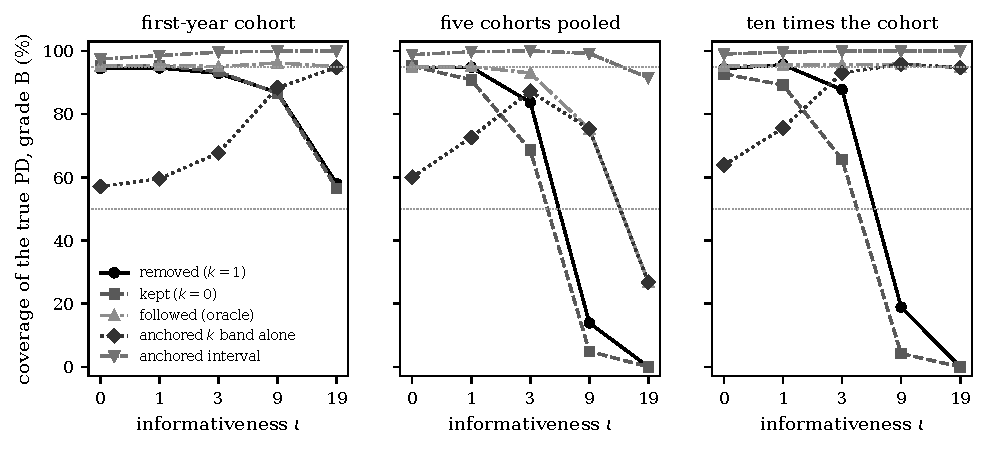
\includegraphics[width=\textwidth]{fig-coverage-k}
\caption{Coverage of grade B's true one-year PD against the informativeness of withdrawal in the generator, for the first annual cohort, the five cohorts pooled and the cohort ten times larger, for removal, keeping, the oracle that follows the \wdn{} ratings, the band of the anchored $k$ alone and the anchored interval; dotted lines mark 95\% and 50\%, 1,000 repetitions per point.}
\label{fig:coverage-k}
\end{figure}

\subsection{Cohort size}

The size of the cohort decides whether a bias can be seen. Table~\ref{tab:scale} and Figure~\ref{fig:scale} raise the first annual cohort from the case's size to thirty times it at informativeness 9. Removal covers \nv{cov.fy.i9.industry}\% at the case's size, \nv{cov.x3.i9.industry}\% at three times, \nv{cov.x10.i9.industry}\% at ten times and \nv{cov.x30.i9.industry}\% at thirty times, as its relative bias of about $-\nv{abias.x30.i9.industry}\%$ stays while its sampling interval shrinks. The oracle covers \nv{cov.x3.i9.followed}\% to \nv{cov.x30.i9.followed}\% throughout, and the anchored interval \nv{cov.x3.i9.anchored}\% to \nv{cov.x30.i9.anchored}\%. The width of the anchored interval shrinks with the cohort, from \nv{w.fy.i9.anchored} to \nv{w.x30.i9.anchored} percentage points, in a ratio to the oracle's width that stays near two; the Manski band hardly shrinks, from \nv{w.fy.i9.identified} to \nv{w.x30.i9.identified}, because its width is set by the share of \wdn{} ratings and not by the number of ratings.

\begin{table}[htbp]
\centering
\footnotesize
\caption{Coverage (\%) of grade B's true one-year PD at informativeness 9 as the cohort grows from the case's size to thirty times it, for the removed, followed and anchored treatments with Monte Carlo standard errors, and the mean widths in percentage points of the anchored interval, the followed interval and the Manski band.}
\label{tab:scale}
\begin{tabular}{llrrrrrr}
\toprule
Cohort & Reps & Removed & Followed & Anchored & $W_{\rm anch}$ & $W_{\rm fol}$ & $W_{\rm Manski}$ \\
\midrule
$\times1$ & 1,000 & $86.8\pm1.1$ & $96.2\pm0.6$ & $99.9\pm0.1$ & 2.16 & 1.13 & 8.26 \\
$\times3$ & 500 & $66.8\pm2.1$ & $96.2\pm0.9$ & $100.0\pm0.0$ & 1.29 & 0.66 & 7.10 \\
$\times10$ & 1,000 & $18.9\pm1.2$ & $95.8\pm0.6$ & $100.0\pm0.0$ & 0.72 & 0.36 & 6.63 \\
$\times30$ & 500 & $0.0\pm0.0$ & $94.2\pm1.0$ & $100.0\pm0.0$ & 0.41 & 0.21 & 6.39 \\
\bottomrule
\end{tabular}
\end{table}


\begin{figure}[htbp]
\centering
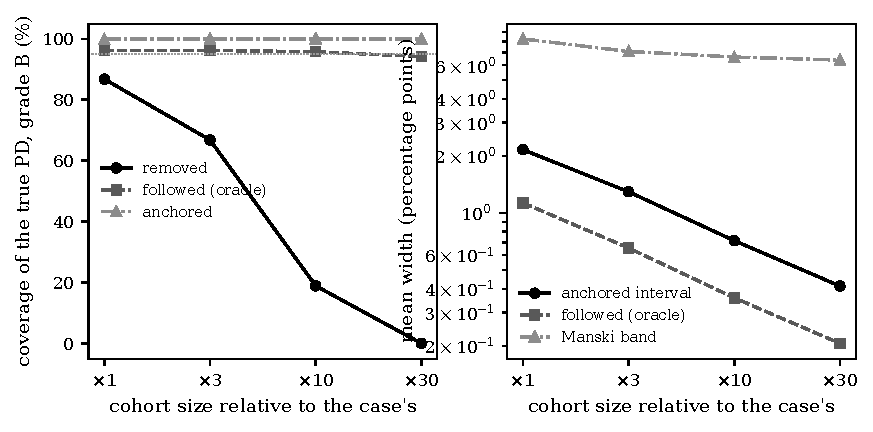
\includegraphics[width=0.9\textwidth]{fig-scale}
\caption{Coverage of grade B's true PD and mean interval width as the first annual cohort grows from the case's size to thirty times it at informativeness 9; left, coverage of removal, the oracle that follows the \wdn{} ratings and the anchored interval; right, the widths of the anchored interval, the oracle's interval and the Manski band on a logarithmic axis.}
\label{fig:scale}
\end{figure}

\subsection{A second source with another definition}

The coverage results above use a second source that counts exactly the followed cohort's defaults. Table~\ref{tab:capture} and Figure~\ref{fig:capture} vary that count at informativeness 9: the second source counts a share $c$ of the defaults, or the defaults and other events. The coverage of the anchored interval is robust: \nv{cap.i9.c0.5.cov}\% at $c=0.5$, \nv{cap.i9.c0.8.cov}\% at 0.8, \nv{cap.i9.c1.1.cov}\% at 1.1 and \nv{cap.i9.c1.3.cov}\% at 1.3, as the interval is wide and always contains the oracle's Jeffreys interval for the count it is given. The centre is not. The relative bias of the anchored point is $\nv{cap.i9.c0.8.bias}\%$ at 0.8, $\nv{cap.i9.c0.9.bias}\%$ at 0.9, $+\nv{cap.i9.c1.1.abias}\%$ at 1.1 and $+\nv{cap.i9.c1.3.abias}\%$ at 1.3, as Proposition~\ref{prop:capture} predicts, and the median anchored odds ratio moves from \nv{cap.i9.c0.8.k} to \nv{cap.i9.c1.3.k} against a realised \nv{ktrue.fy.i9}. A source with a capture of 0.5 or 0.7 returns the odds ratio 0 in the median repetition, because it counts fewer defaults than the transition page already saw, and the point sits at the floor of keeping. The window in which anchoring beats removal on bias is $\nv{rho.fy.i9}<c<\nv{rho.hi.fy.i9}$, which this ladder confirms for $c=1.3$: it is outside the window and has a larger bias than removal's $\nv{bias.fy.i9.industry}\%$. The point $c=0.7$ is also outside it, with a bias of $\nv{cap.i9.c0.7.bias}\%$, which differs from removal's by less than twice their standard errors, so it is at removal's level. At informativeness 3 (the lighter lines of Figure~\ref{fig:capture}) the pattern is the same: the anchored coverage is \nv{cap.i3.c0.5.cov}\% at $c=0.5$ and \nv{cap.i3.c1.3.cov}\% at 1.3, and the bias at 1.3 is $+\nv{cap.i3.c1.3.abias}\%$ against $\nv{bias.fy.i3.industry}\%$ for removal.

\begin{table}[htbp]
\centering
\small
\caption{Grade B at informativeness 9 when the second source counts $c$ times the true defaults (below 1) or counts them and other events at rate $c-1$ (above 1): coverage of the anchored interval with its standard error, coverage of the band alone, mean width, relative bias of the anchored point and the median anchored odds ratio, the realised one being the exact-source row.}
\label{tab:capture}
\begin{tabular}{lrrrrr}
\toprule
Capture $c$ & Anchored (\%) & Band alone (\%) & Width (pp) & Bias (\%) & Median $k$ \\
\midrule
0.5 & $97.5\pm0.5$ & 34.2 & 1.29 & $-25.3$ & 0.0 \\
0.7 & $99.7\pm0.2$ & 71.5 & 1.63 & $-21.8$ & 0.0 \\
0.8 & $99.9\pm0.1$ & 81.1 & 1.82 & $-16.6$ & 1.2 \\
0.9 & $99.8\pm0.1$ & 86.7 & 1.99 & $-9.1$ & 3.2 \\
1 (exact) & $99.9\pm0.1$ & 88.3 & 2.16 & $-0.1$ & 5.2 \\
1.1 & $99.9\pm0.1$ & 87.0 & 2.30 & $+9.5$ & 7.2 \\
1.3 & $97.8\pm0.5$ & 71.8 & 2.56 & $+29.7$ & 12.1 \\
\bottomrule
\end{tabular}
\end{table}


\begin{figure}[htbp]
\centering
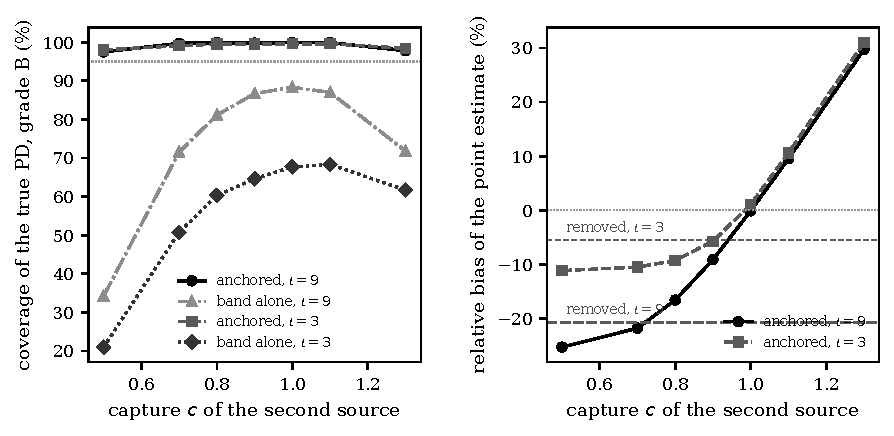
\includegraphics[width=0.95\textwidth]{fig-capture}
\caption{Grade B at informativeness 3 and 9 when the second source counts a share $c$ of the true defaults (below 1) or the defaults and other events (above 1); left, coverage of the anchored interval and of the band alone; right, relative bias of the anchored point, with the bias of removal as horizontal lines; 1,000 repetitions per point.}
\label{fig:capture}
\end{figure}

\subsection{Decisions at a threshold}

A validator uses the PD to decide, so Table~\ref{tab:decisions} and Figure~\ref{fig:decisions} classify each repetition's interval against thresholds set 15 and 30\% below and above the true PD. The removed estimate commits mistakes where the bias runs against the threshold: in the pooled design at informativeness 9 its interval lies wholly below a threshold 15\% under the true PD in \nv{dec.pool.i9.industry.-0.15.w}\% of the repetitions, saying that the PD is below a value it exceeds. The anchored interval never lands on the wrong side in any of the twelve cells of the table, but it is across the threshold in \nv{dec.fy.i9.anchored.-0.15.u}\% of the repetitions at a 15\% offset in the first annual cohort, and in \nv{dec.pool.i9.anchored.-0.15.u}\% when pooled. At ten times the cohort it separates a threshold 30\% below the true PD in \nv{dec.x10.i9.anchored.-0.30.c}\% of the repetitions and one 30\% above in \nv{dec.x10.i9.anchored.+0.30.c}\%. At the case's size the method is silent rather than wrong: the interval tells the validator that the decision cannot be taken from the transition page and one second source.

\begin{table}[htbp]
\centering
\footnotesize
\caption{Threshold decisions on grade B at informativeness 9, for a threshold $t=\mathrm{PD}(1+\delta)$ around the true PD: the percentage of 1,000 repetitions in which the 95\% interval lies on the correct side, on the wrong side, or across the threshold (correct / wrong / undetermined).}
\label{tab:decisions}
\begin{tabular}{llrrrr}
\toprule
Design & Treatment & $\delta=-0.30$ & $\delta=-0.15$ & $\delta=+0.15$ & $\delta=+0.30$ \\
\midrule
first-year cohort & Removed & 6 / 1 / 93 & 1 / 4 / 94 & 25 / 0 / 75 & 45 / 0 / 55 \\
 & Followed (oracle) & 28 / 0 / 72 & 9 / 1 / 90 & 6 / 1 / 93 & 17 / 0 / 83 \\
 & Anchored & 4 / 0 / 96 & 1 / 0 / 99 & 0 / 0 / 100 & 0 / 0 / 100 \\
five cohorts pooled & Removed & 0 / 7 / 93 & 0 / 45 / 55 & 99 / 0 / 1 & 100 / 0 / 0 \\
 & Followed (oracle) & 27 / 0 / 73 & 2 / 3 / 96 & 72 / 0 / 28 & 96 / 0 / 4 \\
 & Anchored & 0 / 0 / 100 & 0 / 0 / 100 & 7 / 0 / 93 & 36 / 0 / 64 \\
ten times the cohort & Removed & 23 / 0 / 77 & 0 / 15 / 85 & 100 / 0 / 0 & 100 / 0 / 0 \\
 & Followed (oracle) & 99 / 0 / 1 & 52 / 0 / 48 & 45 / 0 / 55 & 96 / 0 / 4 \\
 & Anchored & 64 / 0 / 36 & 2 / 0 / 98 & 2 / 0 / 98 & 36 / 0 / 64 \\
\bottomrule
\end{tabular}
\end{table}


\begin{figure}[htbp]
\centering
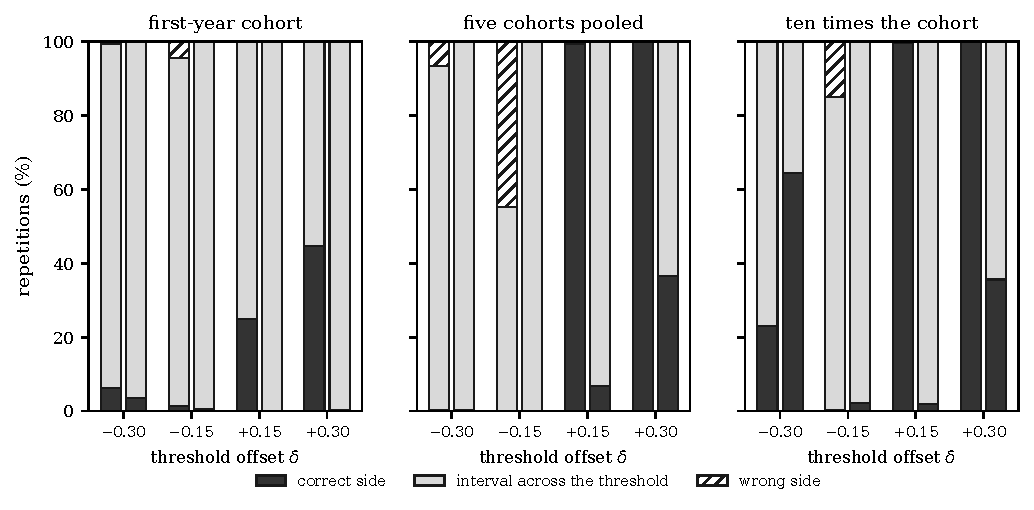
\includegraphics[width=\textwidth]{fig-decisions}
\caption{Threshold decisions on grade B at informativeness 9: for each offset of the threshold from the true PD, the share of 1,000 repetitions in which the interval of the removed estimate (left bar) and of the anchored interval (right bar) lies on the correct side, across the threshold, or on the wrong side, in the three designs.}
\label{fig:decisions}
\end{figure}

\subsection{Agency cohorts}

Table~\ref{tab:real} gives the anchored result on the agencies' cohorts, with the default page as the second source. For S\&P's grade B, pooled over the \nv{real.sp.cohorts} annual cohorts, the transition page counts $D=\nv{real.sp.B.D}$ defaults, $S=\nv{real.sp.B.S}$ survivors and $W=\nv{real.sp.B.W}$ \wdn{} ratings, and the default page counts $A=\nv{real.sp.B.A}$ defaults over $N_a=\nv{real.sp.B.Na}$ ratings. Removal gives a PD of \nv{real.sp.B.pdind}\%; the anchored PD is \nv{real.sp.B.pdanc}\%, with an interval from \nv{real.sp.B.pdlo}\% to \nv{real.sp.B.pdhi}\%. The pooled anchored odds ratio is \nv{real.sp.B.k}, with a band from \nv{real.sp.B.klo} to \nv{real.sp.B.khi}. Figure~\ref{fig:pd-curve} places these on the family: the anchored point lies where the curve has risen to the second source's count, and the tipping $\tip$ to the next grade is \nv{real.sp.B.tip}, a little above the anchored band, so the anchored PD of B does not reach the threshold of \nv{real.sp.B.tipthr}\% that separates it from CCC to C.

\begin{figure}[htbp]
\centering
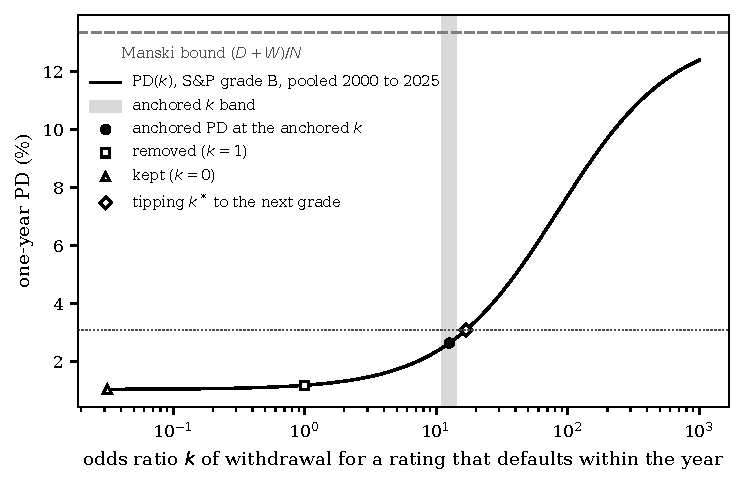
\includegraphics[width=0.85\textwidth]{fig-pd-curve}
\caption{The family PD$(k)$ of S\&P's grade B pooled over all annual cohorts, from the transition page's counts of defaults, survivors and \wdn{} ratings, with the removed estimate, the kept estimate, Manski's bound, the anchored odds ratio with its band and the tipping odds ratio at the threshold to the next grade.}
\label{fig:pd-curve}
\end{figure}

\begin{table}[htbp]
\centering
\footnotesize
\caption{Anchored withdrawal bounds on the agencies' real cohorts of ESMA's central repository, the default page as the second source of the transition page: the pooled PD with withdrawals removed, the anchored PD with its interval, the pooled anchored odds ratio with its band, the cohorts whose band contains it, and the tipping odds ratio that moves the grade to the next one.}
\label{tab:real}
\begin{tabular}{llrp{2.4cm}p{2.6cm}rr}
\toprule
Agency & Grade & PD removed (\%) & Anchored PD (\%) & Pooled $k$ (band) & Cohorts holding it & Tipping $k$ \\
\midrule
S\&P & AA & 0.00 & 0.01 (0.00 to 0.06) & 17.2 (0.0 to 93.6) & 1 of 1 & 26.8 \\
 & A & 0.03 & 0.03 (0.02 to 0.08) & 5.0 (0.0 to 20.7) & 4 of 4 & 16.5 \\
 & BBB & 0.08 & 0.12 (0.06 to 0.19) & 7.9 (2.3 to 15.0) & 8 of 9 & 18.6 \\
 & BB & 0.35 & 0.55 (0.39 to 0.74) & 7.5 (4.9 to 10.5) & 14 of 16 & 10.3 \\
 & B & 1.17 & 2.63 (2.31 to 2.97) & 12.6 (11.2 to 14.1) & 17 of 25 & 16.8 \\
 & CCC to C & 8.07 & 27.43 (25.08 to 29.87) & 36.3 (29.2 to 46.4) & 16 of 25 & -- \\
Fitch & BBB & 0.01 & 0.08 (0.03 to 0.17) & 139.3 (80.1 to 223.3) & 1 of 2 & 35.9 \\
 & BB & 0.15 & 0.44 (0.24 to 0.74) & 24.7 (15.4 to 36.6) & 8 of 8 & 11.6 \\
 & B & 0.52 & 2.09 (1.53 to 2.75) & 31.6 (25.3 to 39.1) & 7 of 10 & 18.4 \\
 & CCC to C & 4.07 & 22.16 (18.02 to 26.69) & 61.2 (42.7 to 96.6) & 11 of 12 & -- \\
\bottomrule
\end{tabular}
\end{table}


For S\&P's CCC to C grade, the pooled anchored odds ratio is \nv{real.sp.CCC-C.k} with a band from \nv{real.sp.CCC-C.klo} to \nv{real.sp.CCC-C.khi}, and the anchored PD \nv{real.sp.CCC-C.pdanc}\% against \nv{real.sp.CCC-C.pdind}\% for removal. In the other grades of S\&P the pooled anchored $k$ is \nv{real.sp.AA.k} for AA, \nv{real.sp.A.k} for A, \nv{real.sp.BBB.k} for BBB, \nv{real.sp.BB.k} for BB and \nv{real.sp.B.k} for B, all above 1. The tipping $k$ is where the agencies differ, as Figure~\ref{fig:tipping} shows for every grade: the anchored $k$ of every S\&P grade lies to the left of the diamond, and that of Fitch's grades BBB, BB and B to its right. For S\&P the pooled anchored $k$ is below the tipping $k$ of every grade that has one, for example \nv{real.sp.BB.k} against \nv{real.sp.BB.tip} for BB, and only the upper end of the band reaches it, in grades AA, A and BB, where the band of grade BB ends at \nv{real.sp.BB.khi}. For Fitch the anchored $k$ is above the tipping $k$ in grades BBB, BB and B, so the anchored PD of each lies beyond the next notch: for BB, $\widehat k=\nv{real.fitch.BB.k}$ against $\tip=\nv{real.fitch.BB.tip}$. The default categories of Fitch's transition pages hold no rating in \nv{fitch.empty.n} of its \nv{real.fitch.cohorts} years, \nv{fitch.empty.first} to \nv{fitch.empty.last}, while its default page counts \nv{fitch.empty.lost} defaulted ratings in them; those ratings sit among the \wdn{} ones, so the anchored $k$ of Fitch measures the definition of its transition page as much as informative withdrawal.

Figure~\ref{fig:forest} shows the annual anchored $k$ with its band for S\&P's grades B and CCC to C and for Fitch's grade B, against the pooled value. The annual values range widely and the bands are wide, which is a sampling effect, but for the two S\&P grades the pooled value lies outside the annual band in a third of the years.

\begin{figure}[htbp]
\centering
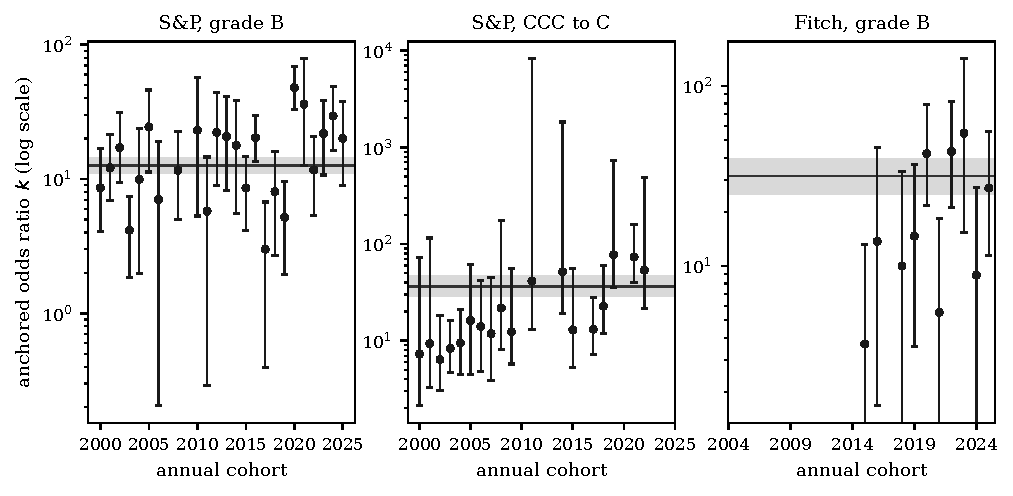
\includegraphics[width=\textwidth]{fig-forest}
\caption{Anchored odds ratio $k$ of each annual cohort with its band, on a logarithmic axis, for S\&P grade B, S\&P grade CCC to C and Fitch grade B, against the pooled anchored odds ratio and its band (horizontal line and shaded area); the default page of the repository is the second source.}
\label{fig:forest}
\end{figure}

\begin{figure}[htbp]
\centering
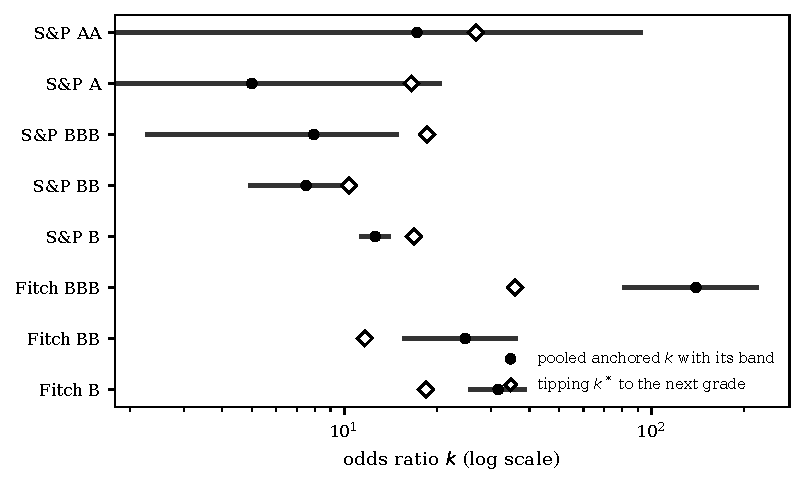
\includegraphics[width=0.85\textwidth]{fig-tipping}
\caption{Pooled anchored odds ratio with its band (circle and segment) and tipping odds ratio to the next grade (diamond), on a logarithmic axis, for each grade of S\&P and Fitch that has an anchored value; where the band lies to the right of the diamond the anchored PD is beyond the next notch of the scale.}
\label{fig:tipping}
\end{figure}

\subsection{Stability of the anchored odds ratio}

The criterion of Equation~\eqref{eq:stability} fails for the agencies' cohorts: \nv{real.sp.B.contain} of \nv{real.sp.B.usable} annual cohorts of S\&P's grade B hold the pooled $k$ in their band, \nv{real.sp.B.share}\%, and \nv{real.sp.CCC-C.contain} of \nv{real.sp.CCC-C.usable} of CCC to C, \nv{real.sp.CCC-C.share}\%; grades BB and BBB of S\&P pass with \nv{real.sp.BB.share}\% and \nv{real.sp.BBB.share}\%. For Fitch, grade B has \nv{real.fitch.B.contain} of \nv{real.fitch.B.usable} and grade BBB \nv{real.fitch.BBB.contain} of \nv{real.fitch.BBB.usable}, on two usable cohorts only. Table~\ref{tab:stability} and Figure~\ref{fig:stability} ask where that instability can come from, by applying the same criterion on known truth. With an exact second source the share of cohorts that hold the pooled $k$ is \nv{stab.i9.c1.B.share}\% in grade B at informativeness 9 and \nv{stab.i3.c1.B.share}\% at 3, so sampling noise alone does not produce it. A second source that counts a constant multiple of the defaults gives \nv{stab.i9.c1.3.B.share}\% at 9 (the series at 1.3 times of Figure~\ref{fig:stability}), and one whose multiple is drawn each year from 1.0 to 1.6 gives \nv{stab.i9.cu1.0-1.6.B.share}\%. When the multiple is drawn each year from 1.0 to 4.0, the share falls to \nv{stab.i9.cu1.0-4.0.B.share}\% for grade B, \nv{stab.i9.cu1.0-4.0.BB.share}\% for BB and \nv{stab.i9.cu1.0-4.0.CCC-C.share}\% for CCC to C (at informativeness 3, \nv{stab.i3.cu1.0-4.0.B.share}\% for grade B).

These multiples scale the followed count $D+X$, not the count $D$ of the transition page, so they are not on the scale of the ratio observed on the agency data. That ratio, the default page's rate over the transition page's rate, $(A/N_a)/(D/N)$, runs for S\&P's grade B over its \nv{ratio.B.n} cohorts with defaults from \nv{ratio.B.min} to \nv{ratio.B.max}, with a median of \nv{ratio.B.median}, a mean of \nv{ratio.B.mean} and \nv{ratio.B.above4} cohorts above 4.0; for CCC to C over \nv{ratio.CCC-C.n} cohorts from \nv{ratio.CCC-C.min} to \nv{ratio.CCC-C.max}, with a median of \nv{ratio.CCC-C.median}, a mean of \nv{ratio.CCC-C.mean} and \nv{ratio.CCC-C.above4} cohorts above 4.0; and for BB over \nv{ratio.BB.n} cohorts from \nv{ratio.BB.min} to \nv{ratio.BB.max}, with a median of \nv{ratio.BB.median}. The range of 1.0 to 4.0 is therefore a variation from year to year of the same order, not a matched one. The last series draws each year, for each grade, a multiple of the defaults $D$ that the transition page observes, uniformly between the extremes of that grade's own observed ratio. It is a draw over the observed range and not a resampling of the observed ratios, and it is centred higher than they are: its mean and median are \nv{ratio.B.draw.mean} for grade B against an observed mean of \nv{ratio.B.mean} and median of \nv{ratio.B.median}, with \nv{ratio.B.draw.above4}\% of its mass above 4.0 against \nv{ratio.B.above4} of \nv{ratio.B.n} cohorts, and \nv{ratio.CCC-C.draw.mean} for CCC to C against \nv{ratio.CCC-C.mean} and \nv{ratio.CCC-C.median}. Under it the share of cohorts that hold the pooled $k$ is, at informativeness 9, \nv{stab.i9.cdobs.B.share}\% for grade B against \nv{real.sp.B.share}\% observed, \nv{stab.i9.cdobs.BB.share}\% for BB against \nv{real.sp.BB.share}\%, and \nv{stab.i9.cdobs.CCC-C.share}\% for CCC to C against \nv{real.sp.CCC-C.share}\%; \nv{stab.i9.cdobs.B.stable}\%, \nv{stab.i9.cdobs.BB.stable}\% and \nv{stab.i9.cdobs.CCC-C.stable}\% of the repetitions of the three grades reach the 80\% criterion. The CCC to C figures are over the \nv{stab.i9.cdobs.CCC-C.defined} repetitions at informativeness 9 (\nv{stab.i3.cdobs.CCC-C.defined} at 3) in which a share is defined, and at informativeness 3 the pooled $k$ of CCC to C is infinite in every repetition. The level of the draw is also above the observed one: the median pooled $k$ of grade B is \nv{stab.i9.cdobs.B.k} against the \nv{real.sp.B.k} observed. A definition gap that varies by year over the range observed for grade B therefore brings its share near the observed one, although the draw is centred above the observed ratios; the same study over the range observed for CCC to C leaves its share above the observed one and does not make it fail, and the gap does not make BB fail, as the observed BB does not. The instability of the anchored $k$ for grade B has the size that a year-to-year change in the definition gap produces and not the size that sampling produces; that this change is its cause is not shown, and what makes the anchored $k$ of CCC to C unstable is not explained by this study (Section~\ref{sec:limitations}).

\begin{table}[htbp]
\centering
\footnotesize
\caption{Stability criterion on known truth: over 1,000 repetitions of five annual cohorts, the mean share of cohorts whose anchored $k$ band contains the pooled anchored $k$ with its standard error, the share of repetitions that reach the 80\% criterion, and the median pooled anchored $k$, at informativeness 3 (panel a) and 9 (panel b) for five second sources: exact; counting 1.3 times the defaults every year; a multiple of the defaults drawn each year from 1.0 to 1.6 and from 1.0 to 4.0; and a multiple of the defaults the transition page observes drawn each year from the range of the grade's own observed ratio of the default page's rate to the transition page's rate, uniform on 0.97 to 5.00 for BB, 1.62 to 7.00 for B and 2.05 to 9.81 for CCC to C. A dash is a median pooled $k$ that is undefined: the pooled $k$ is infinite in every repetition, because the second source counts more defaults than the cohorts' defaults and withdrawals together. Where fewer than 1,000 repetitions have a share (a grade without a usable cohort), the figures are over the repetitions defined: 367 at fewest.}
\label{tab:stability}
\textbf{(a) Informativeness $\iota=3$}\par\smallskip
\begin{tabular}{p{4.2cm}lp{2.4cm}p{2.0cm}r}
\toprule
Capture & Grade & Cohorts holding pooled $k$ (\%) & Repetitions stable (\%) & Median pooled $k$ \\
\midrule
exact & BB & $100.0\pm0.0$ & 99.9 & 1.8 \\
 & B & $100.0\pm0.0$ & 100.0 & 2.2 \\
 & CCC to C & $100.0\pm0.0$ & 100.0 & 1.8 \\
1.3 times & BB & $99.8\pm0.1$ & 99.5 & 7.5 \\
 & B & $99.7\pm0.1$ & 100.0 & 8.0 \\
 & CCC to C & $99.9\pm0.0$ & 100.0 & 11.4 \\
1.0 to 1.6 by year & BB & $99.4\pm0.1$ & 99.2 & 7.3 \\
 & B & $98.7\pm0.2$ & 99.6 & 8.0 \\
 & CCC to C & $97.9\pm0.2$ & 99.4 & 11.2 \\
1.0 to 4.0 by year & BB & $90.4\pm0.5$ & 83.3 & 31.0 \\
 & B & $64.5\pm0.7$ & 39.4 & 40.8 \\
 & CCC to C & $82.0\pm0.9$ & 63.1 & 72.6 \\
observed ratio range of the grade, by year & BB & $93.5\pm0.4$ & 89.4 & 34.6 \\
 & B & $53.8\pm0.7$ & 21.1 & 111.3 \\
 & CCC to C & $99.2\pm0.4$ & 98.9 & -- \\
\bottomrule
\end{tabular}
\medskip

\textbf{(b) Informativeness $\iota=9$}\par\smallskip
\begin{tabular}{p{4.2cm}lp{2.4cm}p{2.0cm}r}
\toprule
Capture & Grade & Cohorts holding pooled $k$ (\%) & Repetitions stable (\%) & Median pooled $k$ \\
\midrule
exact & BB & $99.8\pm0.1$ & 99.8 & 5.8 \\
 & B & $99.5\pm0.1$ & 100.0 & 5.8 \\
 & CCC to C & $99.8\pm0.1$ & 100.0 & 4.4 \\
1.3 times & BB & $99.0\pm0.2$ & 98.4 & 12.5 \\
 & B & $98.2\pm0.2$ & 99.6 & 12.8 \\
 & CCC to C & $99.3\pm0.1$ & 100.0 & 14.1 \\
1.0 to 1.6 by year & BB & $98.4\pm0.2$ & 97.3 & 12.6 \\
 & B & $96.6\pm0.3$ & 98.6 & 12.9 \\
 & CCC to C & $97.2\pm0.2$ & 99.5 & 13.8 \\
1.0 to 4.0 by year & BB & $86.9\pm0.6$ & 72.5 & 42.1 \\
 & B & $64.7\pm0.7$ & 41.1 & 49.8 \\
 & CCC to C & $76.2\pm0.9$ & 48.2 & 103.2 \\
observed ratio range of the grade, by year & BB & $97.2\pm0.3$ & 95.6 & 33.6 \\
 & B & $61.2\pm0.7$ & 33.5 & 76.2 \\
 & CCC to C & $89.7\pm0.9$ & 83.9 & 221.4 \\
\bottomrule
\end{tabular}
\end{table}


\begin{figure}[htbp]
\centering
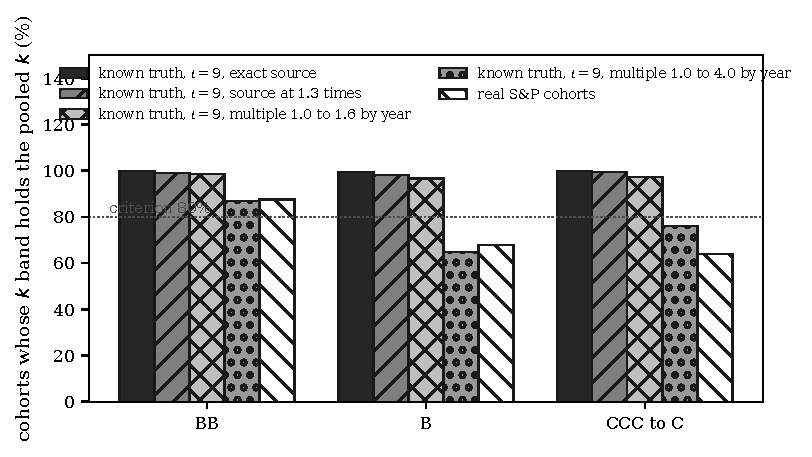
\includegraphics[width=0.85\textwidth]{fig-stability}
\caption{Share of annual cohorts whose anchored $k$ band contains the pooled anchored $k$, by grade: on known truth at informativeness 9 with an exact second source, a second source at 1.3 times the defaults, a multiple of the defaults drawn each year from 1.0 to 1.6 and from 1.0 to 4.0, and a multiple of the observed defaults drawn each year over the range of the grade's own observed ratio, and on the real cohorts of S\&P; the dotted line is the 80\% criterion.}
\label{fig:stability}
\end{figure}

\subsection{Outcome of each prediction}

Table~\ref{tab:hypotheses} sets the predictions of Section~\ref{sec:experimental-design} against the measurements. H1 holds: the anchored interval covers between \nv{h1.min}\% and 100\% of the repetitions at informativeness 1, 3 and 9 in the first-year, pooled and ten-fold designs (the product's criterion reads the ten-fold design at 9 only; at 1 and 3 it gives \nv{cov.x10.i1.anchored}\% and \nv{cov.x10.i3.anchored}\%). In the first-year and ten-fold designs Proposition~\ref{prop:containment} makes this certain for an exact second source; in the pooled design it is an empirical result. H2 holds for removal and keeping only where the bias outgrows the noise, in the pooled and ten-fold designs, and fails in the first annual cohort, where they cover \nv{cov.fy.i9.industry}\% and \nv{cov.fy.i9.unfollowed}\%; the oracle that follows the \wdn{} ratings, which the product reports apart, is under 50\% in none of the three designs.

H3 fails as worded. Against the removed, kept and followed treatments, the comparison of the product's committed criterion, it holds in all three designs, by margins of \nv{h3.single.fy}, \nv{h3.single.pool} and \nv{h3.single.x10} points. Against the Manski band, a published treatment run on the same draws, the anchored interval does not cover more often: the difference in coverage is \nv{h3.man.fy} points in the first annual cohort, \nv{h3.man.pool} points in the pooled design, where the band covers \nv{cov.pool.i9.identified}\% against \nv{cov.pool.i9.anchored}\% and the gap exceeds twice the larger standard error, and \nv{h3.man.x10} points in the ten-fold cohort. What the anchored interval buys against the band is width and not coverage: at informativeness 9 it is \nv{wr.fy.i9}, \nv{wr.pool.i9} and \nv{wr.x10.i9} times narrower than the band in the three designs (\nv{w.fy.i9.anchored} against \nv{w.fy.i9.identified}, \nv{w.pool.i9.anchored} against \nv{w.pool.i9.identified} and \nv{w.x10.i9.anchored} against \nv{w.x10.i9.identified} percentage points). H4 fails: the anchored $k$ of the agencies' grades B and CCC to C is not stable across years, and the instability of grade B has the size of a definition gap that varies by year. H5 holds, with a pooled $k$ of \nv{real.sp.CCC-C.k} and a lower band limit of \nv{real.sp.CCC-C.klo}, both above 1.

The prediction as a whole is refuted. Its refutation clause reads that it is refuted if the anchored interval does not cover more than the existing treatments or if the anchored odds ratio is unstable across years. Both refutation conditions are met: the anchored odds ratio is unstable across years on the agencies' data (H4), and the anchored interval does not cover more than the Manski band (H3). On known truth the coverage clauses hold against the single-answer treatments, and the clause that every existing treatment falls under 50\% holds only for removal and keeping where the cohort is large enough.

\begin{table}[htbp]
\centering
\small
\caption{The predictions stated before the experiments and their outcome: the quantity each measures, the value measured in the first-year, pooled and ten-fold designs (in that order where three are given), the criterion, and whether it held at the repetitions of the grid.}
\label{tab:hypotheses}
\begin{tabular}{lp{4.6cm}p{4.2cm}p{1.8cm}p{2.4cm}}
\toprule
Id & Quantity & Measured (\%, or $k$) & Criterion & Outcome \\
\midrule
H1 & \relax anchored coverage at $\iota=1,3,9$ & 98.5 to 100.0 & at least 90 & holds \\
H2 & \relax removed and kept coverage at $\iota=9$ & first-year cohort 87/87; five cohorts pooled 14/5; ten times the cohort 19/4 & under 50 & holds in two of three designs \\
H2' & \relax followed (oracle) coverage at $\iota=9$ & 96; 75; 96 & under 50 & fails in all three \\
H3 & \relax anchored minus best existing coverage at $\iota=9$ & +3.7; +23.9; +4.2 & above 0 & holds \\
H4 & \relax share of cohorts whose band holds the pooled $k$, S\&P grade B and CCC to C & 68; 64 & at least 80 & fails \\
H5 & \relax pooled anchored $k$ of CCC to C, S\&P & 36.3 & above 1 & holds \\
\bottomrule
\end{tabular}
\end{table}



\section{Ablation}
\label{sec:ablation}
The anchored interval of Equation~\eqref{eq:interval} has four parts: the family PD$(k)$ and its identified band, the second source that anchors $k$, the band of the anchored $k$ clipped to the identified set, and the outer Jeffreys limits. Table~\ref{tab:ablation} removes them one at a time at informativeness 1, where withdrawal is nearly uninformative, and at 9, where it is strongly informative, in the three designs of the coverage grid. The first row of each block is the baseline without any of the parts: the removed estimate with a Jeffreys interval.

\begin{table}[htbp]
\centering
\small
\caption{Ablation on grade B at informativeness 1 and 9: coverage (\%) in the first-year, pooled and ten-fold designs, and the width (percentage points) and relative bias of the first-year design, as the second source, the family PD$(k)$, the clipping to the identified set and the outer Jeffreys interval are retained or removed.}
\label{tab:ablation}
\begin{tabular}{p{0.9cm}p{6.1cm}rrrrr}
\toprule
 & Components retained & First & Pooled & $\times10$ & $W$ (pp) & Bias (\%) \\
\midrule
$\iota=1$ & Removed estimate with a Jeffreys interval (no anchor, no family) & 94.6 & 94.8 & 95.6 & 1.17 & $-0.2$ \\
 & Manski band (family and its bounds, no anchor) & 98.5 & 99.7 & 99.7 & 7.75 & -- \\
 & \relax Anchored $k$ band alone, mapped through PD$(k)$ and clipped to the identified set & 59.5 & 72.6 & 75.6 & 0.74 & $-0.0$ \\
 & Anchored interval (band, clipping and outer Jeffreys interval) & 98.5 & 99.7 & 99.6 & 1.99 & $-0.0$ \\
$\iota=9$ & Removed estimate with a Jeffreys interval (no anchor, no family) & 86.8 & 13.9 & 18.9 & 1.04 & $-20.8$ \\
 & Manski band (family and its bounds, no anchor) & 99.9 & 100.0 & 100.0 & 8.26 & -- \\
 & \relax Anchored $k$ band alone, mapped through PD$(k)$ and clipped to the identified set & 88.3 & 75.3 & 95.8 & 0.96 & $-0.1$ \\
 & Anchored interval (band, clipping and outer Jeffreys interval) & 99.9 & 99.2 & 100.0 & 2.16 & $-0.1$ \\
\bottomrule
\end{tabular}
\end{table}


The second source is what centres the estimate and narrows the interval. Without it the method keeps the family and the identified band, which covers \nv{cov.fy.i9.identified}\% at informativeness 9 in the first annual cohort and is \nv{w.fy.i9.identified} percentage points wide; the point that goes with it is the removed estimate, with its bias of $\nv{bias.fy.i9.industry}\%$. With the second source the point estimate has a bias of $\nv{bias.fy.i9.anchored}\%$ and the interval is \nv{w.fy.i9.anchored} points wide, \nv{w.x10.i9.anchored} in the cohort ten times larger. The second source therefore buys a reduction in width of about three quarters and the removal of the bias, on the condition of Proposition~\ref{prop:capture}: that it counts what the transition page would count.

The outer Jeffreys limits are what make the interval cover. The band of the anchored $k$ alone, which is the interval $[\pdk(k_{\ell}),\pdk(k_{u})]$ of the sensitivity analysis taken at face value, covers \nv{cov.fy.i9.band}\% at informativeness 9 in the first annual cohort and \nv{cov.fy.i1.band}\% at informativeness 1. The shortfall has a mechanism. The band counts the sampling noise of the second source and passes it through the family, but the family is clipped to the identified set: when the lower limit of the second source's rate is below the observed defaults $D/N$, the band's lower end is set to $D/N$, a value that the true PD is often below, because $D/N$ is itself a noisy count. Adding the Jeffreys limits of the transition page's own counts lowers that end to the Jeffreys limit of $D$ and raises the upper end in the same way, and the coverage rises to \nv{cov.fy.i9.anchored}\% and \nv{cov.fy.i1.anchored}\%. The price is the width: from \nv{w.fy.i9.band} to \nv{w.fy.i9.anchored} percentage points at informativeness 9. A narrower interval that covers at its nominal level would need a construction that treats the two sources' noise jointly rather than in sequence; this is not attempted here.

The clipping to the identified set and the family itself do not appear as separate rows because the engine applies them in every variant: the clipping keeps the point and the limits of the second source inside the interval that the counts allow, and the family is what turns a count from the second source into an odds ratio and a tipping value. The tipping $k$ adds nothing to the coverage; it adds the decision rule of Proposition~\ref{prop:tipping}, whose use the decision experiment of Table~\ref{tab:decisions} measures. The quality of the second source is the component with the largest effect on the centre of the result, and the mismatch ladder of Table~\ref{tab:capture} is its ablation: an exact source gives a bias of $\nv{bias.fy.i9.anchored}\%$, one that counts 0.8 of the defaults $\nv{cap.i9.c0.8.bias}\%$, and one that counts 1.3 times $+\nv{cap.i9.c1.3.abias}\%$, while the coverage stays above \nv{cap.i9.c1.3.cov}\% in all three.


\section{Discussion}
\label{sec:discussion}
\subsection{Why the coverage is what it is}

The coverage of the anchored interval is high by construction. With a second source that counts what the transition page would count if it followed every \wdn{} rating, Proposition~\ref{prop:containment} shows that the interval contains the Jeffreys interval of the oracle, so its coverage cannot be below the oracle's and its width is close to twice the oracle's, the ratio that the numerical check on random cohorts and the experiments both give. In the first-year and ten-fold designs the coverage experiment is thus not a test that the method could have failed; in the pooled design the oracle itself covers \nv{cov.pool.i9.followed}\% and the experiment could have failed, and the interval covered \nv{cov.pool.i9.anchored}\%. The Manski band covers as often or more often in every design, so coverage does not separate the anchored interval from the band; its width does, by a factor of \nv{wr.fy.i9} to \nv{wr.x10.i9}. It measures how far above the nominal level the interval sits, from \nv{cov.fy.i9.anchored}\% at informativeness 9 in the first annual cohort to \nv{cov.x10.i9.anchored}\% in the cohort ten times larger, and what it costs in width. A validator who wants an interval at its nominal level should not use this one; one who wants an interval that does not mislead about what the transition page can say should.

The experiments that could fail the method are those that stress the second source, and they show where it is weak. The coverage survives a second source that counts half or 1.3 times the defaults, as the interval is wide. The centre does not: its bias is that of the capture, and the window in which anchoring beats removal on bias is narrow, from $\rho$ to $2-\rho$ for a removal ratio $\rho$ of \nv{rho.fy.i9}. A validator who knows that the second source counts more events than the transition page, as the default page does, knows the sign of the bias of the anchored point.

\subsection{What the agency cohorts say}

The pooled anchored $k$ of S\&P's CCC to C is \nv{real.sp.CCC-C.k}, and that of grade B \nv{real.sp.B.k}. Taken at face value, withdrawal in these grades would be an order of magnitude more informative than independence, and the PD of grade B would be \nv{real.sp.B.pdanc}\% rather than \nv{real.sp.B.pdind}\%. The stability experiment says that this reading is not warranted, which is consistent with the finding of \citet{cantor2007} that the data they examine support random censoring: an anchored $k$ far above 1 that does not hold across years is better read as the difference between two definitions of default than as informative withdrawal. On known truth, an exact second source gives annual bands that hold the pooled $k$ in \nv{stab.i9.c1.B.share}\% of the cohorts, and a definition gap drawn each year over the range observed for grade B, \nv{ratio.B.min} to \nv{ratio.B.max} times the observed defaults and centred above the observed ratios, brings the share to \nv{stab.i9.cdobs.B.share}\%, near the \nv{real.sp.B.share}\% observed for S\&P's grade B (1.0 to 4.0 times the followed defaults gives \nv{stab.i9.cu1.0-4.0.B.share}\%); drawn over the range observed for CCC to C it leaves the share at \nv{stab.i9.cdobs.CCC-C.share}\%, against \nv{real.sp.CCC-C.share}\% observed. The anchored $k$ of the agencies' cohorts absorbs the difference between the two pages' definitions of default, which changes from year to year, together with whatever informativeness the withdrawals have. It is an anchored $k$ conditional on the two definitions being equivalent, and the repository does not make them so. The case of Fitch is the sharpest: its transition pages hold no defaulted rating in \nv{fitch.empty.n} years while its default page counts \nv{fitch.empty.lost}, so the anchored $k$ of Fitch is mostly a statement about where the defaulted ratings are recorded.

What the agency cohorts do support is the statement that the tipping $k$ matters. For S\&P's grade B, the tipping $k$ to the next grade is \nv{real.sp.B.tip}, and the removal PD would need withdrawal to be that informative to move the grade to the next notch; the anchored $k$, whatever its meaning, is below it. For Fitch's grade BB, the anchored $k$ is \nv{real.fitch.BB.k} against a tipping $k$ of \nv{real.fitch.BB.tip}, and the decision flips under the anchor but only if the definitions agree.

\subsection{Negative results and what they imply}

The prediction as a whole is refuted, by its stability clause on the agencies' data and by its coverage clause against the Manski band. H2 is refuted in part: the clause that removal and keeping cover under 50\% of the repetitions at informativeness 9 fails in the first annual cohort, \nv{cov.fy.i9.industry}\% and \nv{cov.fy.i9.unfollowed}\%, because the bias of about a fifth to a quarter is smaller than the sampling interval of a grade with some sixteen defaults a year. It holds when the cohort is large enough or the years are pooled. H3 fails as worded, because the Manski band covers as often or more often than the anchored interval, which buys width and not coverage. H4 is refuted: the clause on stability fails on the agencies' cohorts. The continuous-time estimator that reads withdrawal as independent censoring has a bias between those of the pooled removal and keeping estimates at informativeness 9, $-\nv{dur.i9.abias}\%$ against $\nv{bias.pool.i9.industry}\%$ and $\nv{bias.pool.i9.unfollowed}\%$, which shows that the problem is not removed by working in continuous time.

For a bank the implications are three. A grade's PD under withdrawal should be reported as the family and its tipping $k$ at the thresholds that matter, which needs no second source and no assumption beyond A1 and A3. The anchored interval should be reported only where the definitions of the two sources have been compared, and with the capture window of Proposition~\ref{prop:capture} stated. And pooling years, the usual practice, brings a selection bias that no estimator of the cohort corrects, and that all the intervals of the paper inherit.


\section{Limitations}
\label{sec:limitations}
\subsection{Internal validity}

The known-truth study has one generator and one design of withdrawal: a Markov chain of seven grades fitted to S\&P's counts, independent obligors, a constant withdrawal hazard of \nv{withdrawal.rate}\% a year raised by the factor $1+\iota$ in the year before default, and a single odds ratio for every rating of a grade, which is assumption A2 built into the data. A generator in which withdrawal depends on a rating's age, on its issuer's size, or on a downgrade that precedes the default, would give a $k$ that varies within a grade, and the coverage of the method under such heterogeneity is not measured. The hypotheses are read on grade B, whose cohort and PD give a typical grade of the speculative range; the grid stores every grade, and for the grades with few defaults, AAA to A, the interval is dominated by the sampling count and the comparison between treatments is not informative, so those grades are not discussed. The comparison with the duration estimator rests on \nv{reps.duration} repetitions and a bootstrap of \nv{boot.duration} replicates, fewer than the other studies; its standard errors are reported and its conclusion, that the bias is larger than removal's, is a bias of several standard errors.

The repetitions of each cell are independent and the standard errors are binomial, so a coverage difference smaller than two standard errors is not called. The experiments run no formal test, and a coverage below nominal by one standard error is not evidence of a failure. The Lemma of Section~\ref{sec:theory} is checked on every count up to the sizes listed and not proved; Proposition~\ref{prop:containment} is conditional on it.

\subsection{External validity}

The agencies' cohorts are the aggregates that ESMA publishes for the European entities of the agencies, in a stock model in which intra-period activity is derived from the ratings at the start and the end of a period. The transition and default pages define default differently, ESMA sets no common definition, and the agencies' definitions may differ among themselves. The second source assumed by the method is therefore never exactly equal to the transition page's count on these data, and the stability result shows how much that matters. Moody's transition page has no default category and cannot be anchored. A PD by grade of an agency is not the PD of a bank's internal grade, and nothing here certifies a rating system; the method is meant for a bank's own cohorts, where the validator can compare the second source's definition with the first before relying on it.

Pooling five annual cohorts, as the product does, means that the realised default fraction of later cohorts is lower than the one-year PD of the generator when withdrawal is informative (Proposition~\ref{prop:selection}), so the coverage of a later-cohort estimate against the first-year truth mixes the method's error with the selection. The first annual cohort and the ten-fold cohort are the designs in which the target is the same as the generator's truth; the pooled design measures what a practitioner who pools gets.

\subsection{Construct validity}

The quantity that the intervals are checked against is the one-year PD of the generator, computed from its matrix exponential, a PD in the sense of a rating followed to the year end. A bank's regulatory PD is a through-the-cycle average that may include more than the first year after a rating, and the anchored odds ratio is defined for one period. The capture ladder models a different definition of default as a thinned or inflated count; a real definition gap differs by grade and year and is not independent of withdrawal, since the agencies' defaulted ratings are often \wdn{} after the default. The year-varying multiples of the stability study are drawn independently across years and grades, and the study shows only that variation of that size is enough to reproduce the observed instability, not that it is the cause.

The width of the anchored interval is a threat to the use of the method: at the case's size the interval is across the threshold in nearly every repetition for offsets of 15\%, so the method rarely decides. This is a finding about the information in the data, and a validator who needs a decision from a single grade and year with the cohort sizes of the case should expect to be told that none can be taken.

\subsection{Scope}

The method is for one period and one grade at a time. It does not model competing exits other than default and withdrawal, it assumes the second source counts the same ratings, and it returns the odds ratio and the interval, not a lifetime PD. Its extension to multi-year horizons would chain periods whose $k$ are not the same and whose cohorts have lost the ratings \wdn{} earlier, which is the selection of Proposition~\ref{prop:selection}; it is not attempted. The method also does not decide which second source to trust: it takes the count of the second source as given and propagates its sampling noise, not the doubt about its definition. When several second sources exist, for instance the default page and the defaults-by-category page of the repository, each gives its own anchored $k$, and the spread among them is a measure of the definition gap that the method reports but does not model, and a validator would read it before reading any single anchored interval.


\section{Reproducibility}
\label{sec:reproducibility}
The code, the data and the computational outputs are in the repository \pth{github.com/fsantibanezleal/CAOS_Contraste}. The method is the module \pth{riskvalidation.transitions.withdrawals} of the engine \pth{riskvalidation} 1.1.0, published on the Python Package Index, and its documentation in the engine repository (\pth{docs/transitions/06_withdrawal-bounds.md}) states the model and the assumptions. The product's study, the real-data function and the criteria of Section~\ref{sec:experimental-design} are in \pth{data-pipeline/pipeline/cases/c04_bounds.py}, and its documents, one per agency and one for the known-truth withdrawals family, are \pth{data/derived/C04/sp.json}, \pth{fitch.json} and \pth{withdrawals.json}. The cohorts are the aggregates of the central repository of ESMA (\pth{registers.esma.europa.eu/cerep-publication}), reproduced as its terms allow with the source acknowledged.

Every number of the paper is read from those documents or from the outputs of the scripts of this paper by the table script, and no number of the prose is typed. From the repository root, with the engine installed in a Python environment,
\begin{itemize}
\item \pth{experiments/extended_study.py} runs the coverage grid, the capture ladder, the stability study, the scale ladder and the duration comparison, each with the option \pth{--only} to run one, and writes the JSON files of \pth{experiments/results/};
\item \pth{experiments/theory_checks.py} runs the numerical checks of the propositions;
\item \pth{experiments/crosscheck_pipeline.py} reproduces the product's committed function on the same seed and compares the coverage of every treatment;
\item \pth{tables/make_tables.py} writes the tables and the file of numbers, and \pth{figures/make_figures.py} the figures, both from the committed documents and the results;
\item \pth{pdflatex}, \pth{bibtex} and two more \pth{pdflatex} runs from the manuscript folder build the paper.
\end{itemize}
Each experiment script runs in under 30 minutes on a workstation, the longest being the coverage grid, and a rerun of the grid with the default repetitions and seeds reproduces its two output files byte for byte. The seeds are pure functions of the case seed \nv{case.seed} and the key of each cell (Table~\ref{tab:design}), so a cell can be rerun alone.


\section{Conclusions}
\label{sec:conclusions}
The PD of a grade under informative rating withdrawals is a curve in the odds ratio $k$ of withdrawal, not a number, and the three treatments in use are three points of it. The curve, its worst-case bound and the tipping $k$ of a decision come in closed form from the transition page alone; a second source that counts the defaults of the same ratings, such as the default page of the ESMA repository, anchors the curve and gives an interval. On rating paths of known truth the anchored interval covers the true PD of grade B in \nv{h1.min}\% to 100\% of \nv{reps} repetitions at informativeness 1, 3 and 9 in the first-year and pooled designs and at 9 in the ten-fold design, against \nv{cov.pool.i9.industry}\% for removal in the pooled design, and it is \nv{w.fy.i9.anchored} percentage points wide in the first annual cohort against \nv{w.fy.i9.followed} for the oracle that follows every withdrawal, which it contains by construction. Its centre is exact when the second source counts exactly what the transition page would count and carries the capture of the second source as a bias otherwise. On the agencies' cohorts, the pooled anchored $k$ is above 1 in every grade, \nv{real.sp.CCC-C.k} for S\&P's CCC to C, but it does not hold across years for S\&P's grades B and CCC to C or for Fitch's grade B, and the instability has the size of a definition gap that changes from year to year, not of sampling. The anchored odds ratio of the agencies is conditional on the two pages defining default alike. The next steps are an interval that treats the noise of the two sources jointly, to narrow the conservative width, a bank's own second source in place of the repository's pages, and a multi-year extension that models the selection of pooled cohorts.


\bibliographystyle{plainnat}
\bibliography{references}

\end{document}
